% Options for packages loaded elsewhere
\PassOptionsToPackage{unicode}{hyperref}
\PassOptionsToPackage{hyphens}{url}
%
\documentclass[
]{book}
\usepackage{lmodern}
\usepackage{amsmath}
\usepackage{ifxetex,ifluatex}
\ifnum 0\ifxetex 1\fi\ifluatex 1\fi=0 % if pdftex
  \usepackage[T1]{fontenc}
  \usepackage[utf8]{inputenc}
  \usepackage{textcomp} % provide euro and other symbols
  \usepackage{amssymb}
\else % if luatex or xetex
  \usepackage{unicode-math}
  \defaultfontfeatures{Scale=MatchLowercase}
  \defaultfontfeatures[\rmfamily]{Ligatures=TeX,Scale=1}
\fi
% Use upquote if available, for straight quotes in verbatim environments
\IfFileExists{upquote.sty}{\usepackage{upquote}}{}
\IfFileExists{microtype.sty}{% use microtype if available
  \usepackage[]{microtype}
  \UseMicrotypeSet[protrusion]{basicmath} % disable protrusion for tt fonts
}{}
\makeatletter
\@ifundefined{KOMAClassName}{% if non-KOMA class
  \IfFileExists{parskip.sty}{%
    \usepackage{parskip}
  }{% else
    \setlength{\parindent}{0pt}
    \setlength{\parskip}{6pt plus 2pt minus 1pt}}
}{% if KOMA class
  \KOMAoptions{parskip=half}}
\makeatother
\usepackage{xcolor}
\IfFileExists{xurl.sty}{\usepackage{xurl}}{} % add URL line breaks if available
\IfFileExists{bookmark.sty}{\usepackage{bookmark}}{\usepackage{hyperref}}
\hypersetup{
  pdftitle={R for Non-Programmers: A Guide for Social Scientists},
  pdfauthor={Daniel Dauber},
  hidelinks,
  pdfcreator={LaTeX via pandoc}}
\urlstyle{same} % disable monospaced font for URLs
\usepackage{color}
\usepackage{fancyvrb}
\newcommand{\VerbBar}{|}
\newcommand{\VERB}{\Verb[commandchars=\\\{\}]}
\DefineVerbatimEnvironment{Highlighting}{Verbatim}{commandchars=\\\{\}}
% Add ',fontsize=\small' for more characters per line
\usepackage{framed}
\definecolor{shadecolor}{RGB}{248,248,248}
\newenvironment{Shaded}{\begin{snugshade}}{\end{snugshade}}
\newcommand{\AlertTok}[1]{\textcolor[rgb]{0.94,0.16,0.16}{#1}}
\newcommand{\AnnotationTok}[1]{\textcolor[rgb]{0.56,0.35,0.01}{\textbf{\textit{#1}}}}
\newcommand{\AttributeTok}[1]{\textcolor[rgb]{0.77,0.63,0.00}{#1}}
\newcommand{\BaseNTok}[1]{\textcolor[rgb]{0.00,0.00,0.81}{#1}}
\newcommand{\BuiltInTok}[1]{#1}
\newcommand{\CharTok}[1]{\textcolor[rgb]{0.31,0.60,0.02}{#1}}
\newcommand{\CommentTok}[1]{\textcolor[rgb]{0.56,0.35,0.01}{\textit{#1}}}
\newcommand{\CommentVarTok}[1]{\textcolor[rgb]{0.56,0.35,0.01}{\textbf{\textit{#1}}}}
\newcommand{\ConstantTok}[1]{\textcolor[rgb]{0.00,0.00,0.00}{#1}}
\newcommand{\ControlFlowTok}[1]{\textcolor[rgb]{0.13,0.29,0.53}{\textbf{#1}}}
\newcommand{\DataTypeTok}[1]{\textcolor[rgb]{0.13,0.29,0.53}{#1}}
\newcommand{\DecValTok}[1]{\textcolor[rgb]{0.00,0.00,0.81}{#1}}
\newcommand{\DocumentationTok}[1]{\textcolor[rgb]{0.56,0.35,0.01}{\textbf{\textit{#1}}}}
\newcommand{\ErrorTok}[1]{\textcolor[rgb]{0.64,0.00,0.00}{\textbf{#1}}}
\newcommand{\ExtensionTok}[1]{#1}
\newcommand{\FloatTok}[1]{\textcolor[rgb]{0.00,0.00,0.81}{#1}}
\newcommand{\FunctionTok}[1]{\textcolor[rgb]{0.00,0.00,0.00}{#1}}
\newcommand{\ImportTok}[1]{#1}
\newcommand{\InformationTok}[1]{\textcolor[rgb]{0.56,0.35,0.01}{\textbf{\textit{#1}}}}
\newcommand{\KeywordTok}[1]{\textcolor[rgb]{0.13,0.29,0.53}{\textbf{#1}}}
\newcommand{\NormalTok}[1]{#1}
\newcommand{\OperatorTok}[1]{\textcolor[rgb]{0.81,0.36,0.00}{\textbf{#1}}}
\newcommand{\OtherTok}[1]{\textcolor[rgb]{0.56,0.35,0.01}{#1}}
\newcommand{\PreprocessorTok}[1]{\textcolor[rgb]{0.56,0.35,0.01}{\textit{#1}}}
\newcommand{\RegionMarkerTok}[1]{#1}
\newcommand{\SpecialCharTok}[1]{\textcolor[rgb]{0.00,0.00,0.00}{#1}}
\newcommand{\SpecialStringTok}[1]{\textcolor[rgb]{0.31,0.60,0.02}{#1}}
\newcommand{\StringTok}[1]{\textcolor[rgb]{0.31,0.60,0.02}{#1}}
\newcommand{\VariableTok}[1]{\textcolor[rgb]{0.00,0.00,0.00}{#1}}
\newcommand{\VerbatimStringTok}[1]{\textcolor[rgb]{0.31,0.60,0.02}{#1}}
\newcommand{\WarningTok}[1]{\textcolor[rgb]{0.56,0.35,0.01}{\textbf{\textit{#1}}}}
\usepackage{longtable,booktabs}
\usepackage{calc} % for calculating minipage widths
% Correct order of tables after \paragraph or \subparagraph
\usepackage{etoolbox}
\makeatletter
\patchcmd\longtable{\par}{\if@noskipsec\mbox{}\fi\par}{}{}
\makeatother
% Allow footnotes in longtable head/foot
\IfFileExists{footnotehyper.sty}{\usepackage{footnotehyper}}{\usepackage{footnote}}
\makesavenoteenv{longtable}
\usepackage{graphicx}
\makeatletter
\def\maxwidth{\ifdim\Gin@nat@width>\linewidth\linewidth\else\Gin@nat@width\fi}
\def\maxheight{\ifdim\Gin@nat@height>\textheight\textheight\else\Gin@nat@height\fi}
\makeatother
% Scale images if necessary, so that they will not overflow the page
% margins by default, and it is still possible to overwrite the defaults
% using explicit options in \includegraphics[width, height, ...]{}
\setkeys{Gin}{width=\maxwidth,height=\maxheight,keepaspectratio}
% Set default figure placement to htbp
\makeatletter
\def\fps@figure{htbp}
\makeatother
\setlength{\emergencystretch}{3em} % prevent overfull lines
\providecommand{\tightlist}{%
  \setlength{\itemsep}{0pt}\setlength{\parskip}{0pt}}
\setcounter{secnumdepth}{5}
\usepackage{booktabs}
\ifluatex
  \usepackage{selnolig}  % disable illegal ligatures
\fi
\usepackage[]{natbib}
\bibliographystyle{apalike}

\title{R for Non-Programmers: A Guide for Social Scientists}
\author{Daniel Dauber}
\date{2021-07-28}

\begin{document}
\maketitle

{
\setcounter{tocdepth}{1}
\tableofcontents
}
\hypertarget{welcome}{%
\chapter*{Welcome 👋}\label{welcome}}
\addcontentsline{toc}{chapter}{Welcome 👋}


\includegraphics{images/chapter_00_img/r_for_non_programmers_logo.png}

Welcome to \emph{R for Non-Programmers: A guide for Social Scientists}. This book is intended to be of help to everyone who wishes to enter the world of R Programming, but not necessarily for the purpose to become a programmer. Instead, this book intends to convey key concepts in data analysis, especially quantitative research.

{[}Add more{]}

\hypertarget{acknowledgments}{%
\chapter*{Acknowledgments 🙏}\label{acknowledgments}}
\addcontentsline{toc}{chapter}{Acknowledgments 🙏}

Special thanks are due to my wife, who supported me in so many ways to get this book completed. Also, I would like to thank my son, who patiently watched me sitting at the computer type this book up.

\hypertarget{readme-before-you-get-started}{%
\chapter{\texorpdfstring{\texttt{Readme.} Before you get started}{Readme. Before you get started}}\label{readme-before-you-get-started}}

\hypertarget{a-starting-point-and-reference-book}{%
\section{A starting point and reference book}\label{a-starting-point-and-reference-book}}

\texttt{to\ be\ added}

\hypertarget{download-the-companion-r-package}{%
\section{Download the companion R package}\label{download-the-companion-r-package}}

\texttt{to\ be\ added}

\begin{itemize}
\item
  Explain where to download
\item
  Explain how examples are shown in this book (code in the first grey box, console results in the second grey box
\end{itemize}

\hypertarget{a-tidyverse-approach-with-some-basic-r}{%
\section{A `tidyverse' approach with some basic R}\label{a-tidyverse-approach-with-some-basic-r}}

\texttt{to\ be\ added}

\hypertarget{why-learn-a-programming-language-as-a-non-programmer}{%
\chapter{Why learn a programming language as a non-programmer?}\label{why-learn-a-programming-language-as-a-non-programmer}}

\emph{`R'}, it is not just a letter you learn in primary school, but a powerful programming language. While it is used for a lot of quantitative data analysis, it has grown over the years to become a powerful tool that excels (\#no-pun-intended) in handling data and performing customised computations with quantitative and qualitative data.

\emph{R}~is now one of my core tools to perform various types of analysis because I can use it in many different ways, for example,

\begin{itemize}
\tightlist
\item
  statistical analysis,
\item
  corpus analysis,
\item
  development of online dashboards to dynamically generate interactive data visualisations,
\item
  connection to social media APIs for data collection,
\item
  Creation of reporting systems to provide individualised feedback to research participants,
\item
  Drafting and writing research articles, etc.
\end{itemize}

\begin{quote}
\emph{Learning R is like learning a foreign language. If you like learning languages, then `R' is just another one.}
\end{quote}

While \emph{R} has become a comprehensive tool for data scientists, it has yet to find its way into the mainstream field of Social Sciences. Why? Well, learning programming languages is not necessarily something that feels comfortable to everyone. It is not like Microsoft Word, where you can open the software and explore it through trial and error. Learning a programming language is like learning a foreign language: You have to learn vocabulary, grammar and syntax. Similar to learning a new language, programming languages also have steep learning curves and require quite some commitment.

For this reason, most people do not even dare to learn it because it is time-consuming and often not considered a \emph{`core method'} in Social Sciences disciplines. Apart from that, tools like SPSS have very intuitive interfaces, which seem much easier to use (or not?). However, the feeling of having \emph{`mastered'} \emph{R} (although one might never be able to claim this) can be extremely rewarding.

I guess this introduction was not necessarily helpful in convincing you to learn any programming language. However, despite those initial hurdles, there are a series of advantages to consider. Below I list some good reasons to learn a programming language as they pertain to my own experiences.

\hypertarget{learning-new-tools-to-analyse-your-data-is-always-essential}{%
\section{Learning new tools to analyse your data is always essential}\label{learning-new-tools-to-analyse-your-data-is-always-essential}}

Theories change over time, and new insights into certain social phenomena are published every day. Thus, your knowledge might get outdated quite quickly. This is not so much the case for research methods knowledge. Typically, analytical techniques remain over many years. We still use the mean, mode, quartiles, standard deviation, etc., to describe our quantitative data. Still, there are always new computational methods that help us to crunch the numbers even more. \emph{R} is a tool that allows you to venture into new analytical territory because it is open source. Thousands of developers provide cutting-edge research methods free of charge for you to try with your data. You can find them on platforms like \href{https://github.com}{GitHub}. \emph{R} is like a giant supermarket, where all products are available for free. However, to read the labels on the product packaging and understand what they are, you have to learn the language used in this supermarket.

\hypertarget{programming-languages-enhance-your-conceptual-thinking}{%
\section{Programming languages enhance your conceptual thinking}\label{programming-languages-enhance-your-conceptual-thinking}}

While I have no empirical evidence for this, I am very certain it is true. While I would argue that my conceptual thinking is quite good, I would not necessarily say that I was born with it. Programming languages are very logical. Any error in your code will make you fail to execute it properly. Sometimes you face challenges in creating the correct code to solve a problem. Through creative abstract thinking (I should copyright this term), you start to approach your problems differently, whether it is a coding problem or a problem in any other context. For example, I know many students enjoy the process of qualitative coding. However, they often struggle to detach their insights from the actual data and synthesise ideas on an abstract and more generic level. Qualitative researchers might refer to this as challenges in '\emph{second-order deconstruction of meaning'}. This process of abstraction is a skill that needs to be honed, nurtured and practised. From my experience, programming languages are one way to achieve this, but they might not be recognised for this just yet.

\hypertarget{programming-languages-allow-you-to-look-at-your-data-from-a-different-angle}{%
\section{Programming languages allow you to look at your data from a different angle}\label{programming-languages-allow-you-to-look-at-your-data-from-a-different-angle}}

There are certainly commonly known and well-established techniques regarding how you should analyse your data rigorously. However, it can be quite some fun to try techniques outside your disciplines. This does not only apply to programming languages, of course. Sometimes, learning about a new research method enables you to look at your current tools in very different ways too. One of the biggest challenges for any researcher is to reflect on your work. Learning new and maybe even \emph{`strange'} tools can help with this. Admittedly, sometimes you might find out that some new tools are also a dead-end. Still, you might have learned something valuable through the process of engaging with your data differently. So shake off the rust of your analytical routine and blow some fresh air into your research methods.

\hypertarget{learning-any-programming-language-will-help-you-learn-other-programming-languages.}{%
\section{Learning any programming language will help you learn other programming languages.}\label{learning-any-programming-language-will-help-you-learn-other-programming-languages.}}

Once you understand the logic of one language, you will find it relatively easy to understand new programming languages. Of course, if you wanted to, you could become the next '\emph{Neo'} (from \href{https://www.imdb.com/title/tt0133093/?ref_=ext_shr_lnk}{`The Matrix')} and change the reality of your research forever. On a more serious note, though, if you know any programming language already, learning R will be easier because you have accrued some basic understanding of these particular types of languages.

Having considered everything of the above, do you feel ready for your next foreign language?

\hypertarget{setting-up-r-and-rstudio}{%
\chapter{Setting up R and RStudio}\label{setting-up-r-and-rstudio}}

Every journey starts with gathering the right equipment. This intellectual journey is not much different. The first step that every '\emph{R} novice has to face is to set everything up to get started. There are essentially two strategies:

\begin{itemize}
\tightlist
\item
  Install \href{https://www.r-project.org}{\emph{R}}and \href{https://www.rstudio.com}{RStudio}
\end{itemize}

or

\begin{itemize}
\tightlist
\item
  Run RStudio in a browser via \href{https://rstudio.cloud}{RStudio Cloud}
\end{itemize}

While installing~\emph{R}~and Studio requires more time and effort, I strongly recommend it, especially if you want to work offline or make good use of your computer's CPU. However, if you are not sure yet whether you enjoy learning~\emph{R}, you might wish to look at RStudio Cloud first. Either way, you can follow the examples of this book no matter which choice you make.

\hypertarget{installing-r}{%
\section{Installing R}\label{installing-r}}

The core module of our programming is R itself, and since it is an open-source project, it is available for free on Windows, Mac and Linux computers. Here is what you need to do to install it properly on your computer of choice:

\begin{enumerate}
\def\labelenumi{\arabic{enumi}.}
\item
  Go to \href{https://www.r-project.org\%5D(https://www.r-project.org)}{www.r-project.org}

  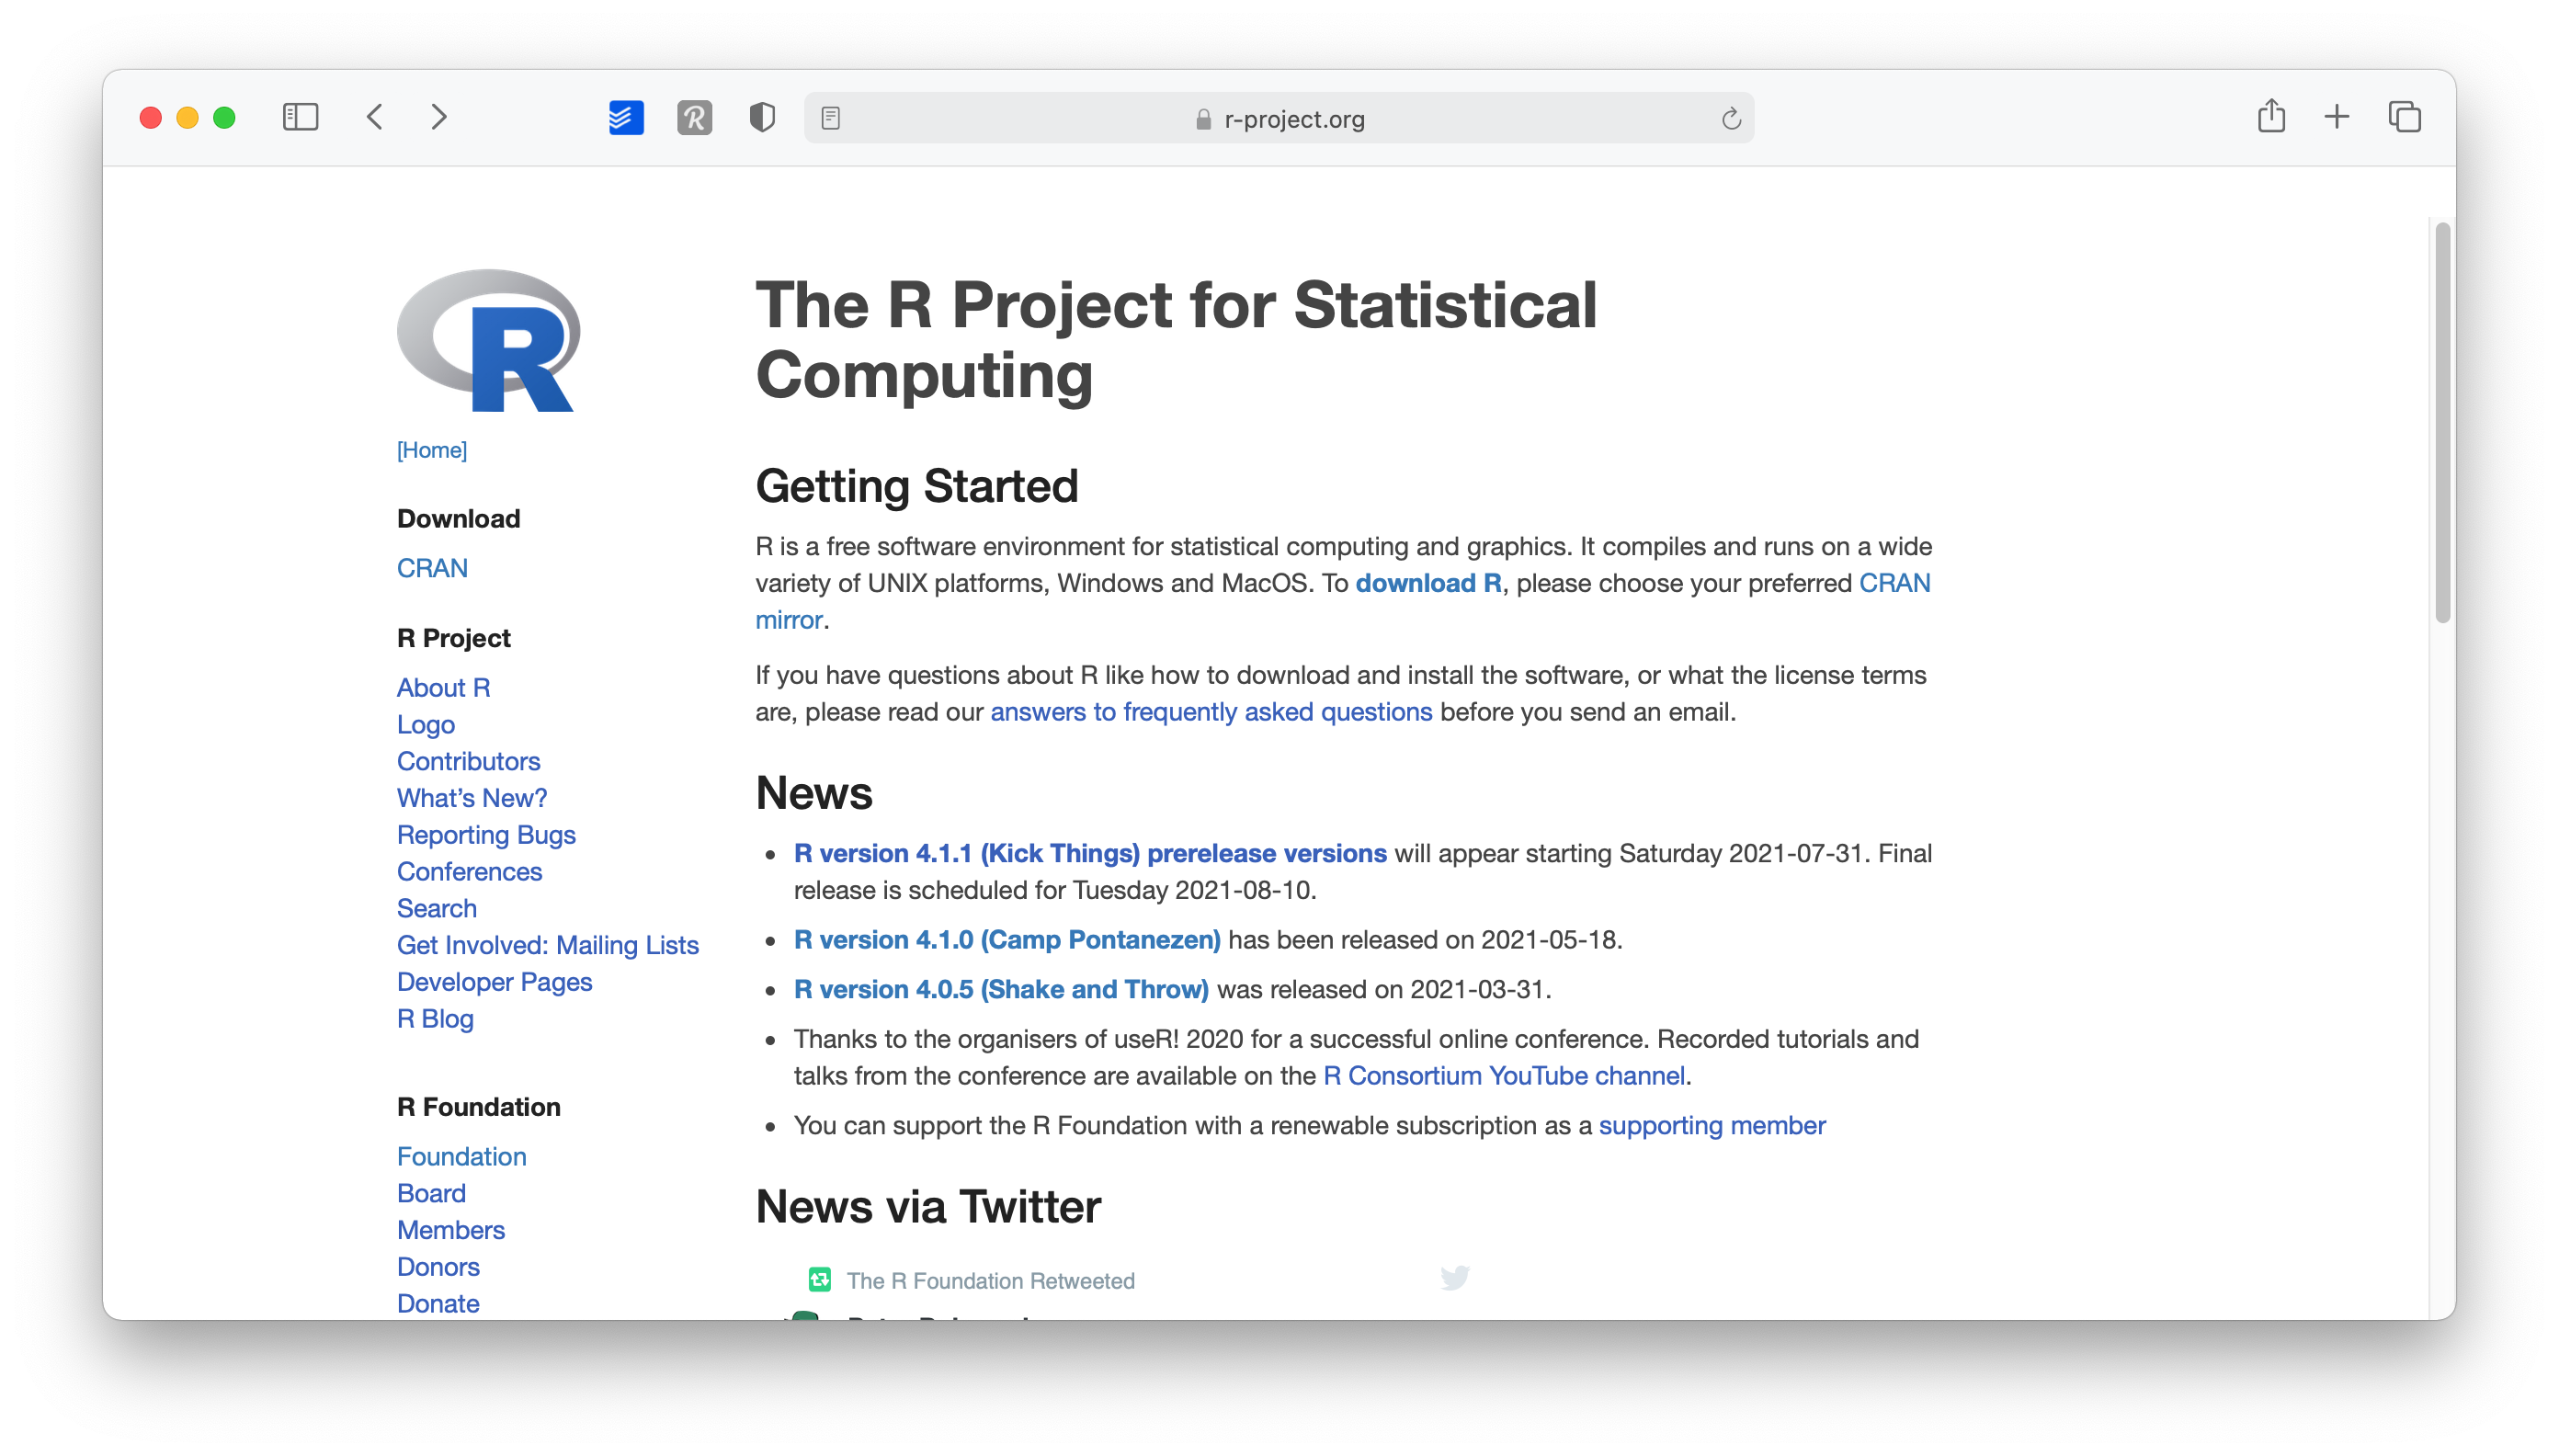
\includegraphics{images/chapter_03_img/r_project/00_r_project_page.png}
\item
  Click on \texttt{CRAN} where it says download.
\item
  Choose a server in your country (all of them work, but downloads will perform quicker).

  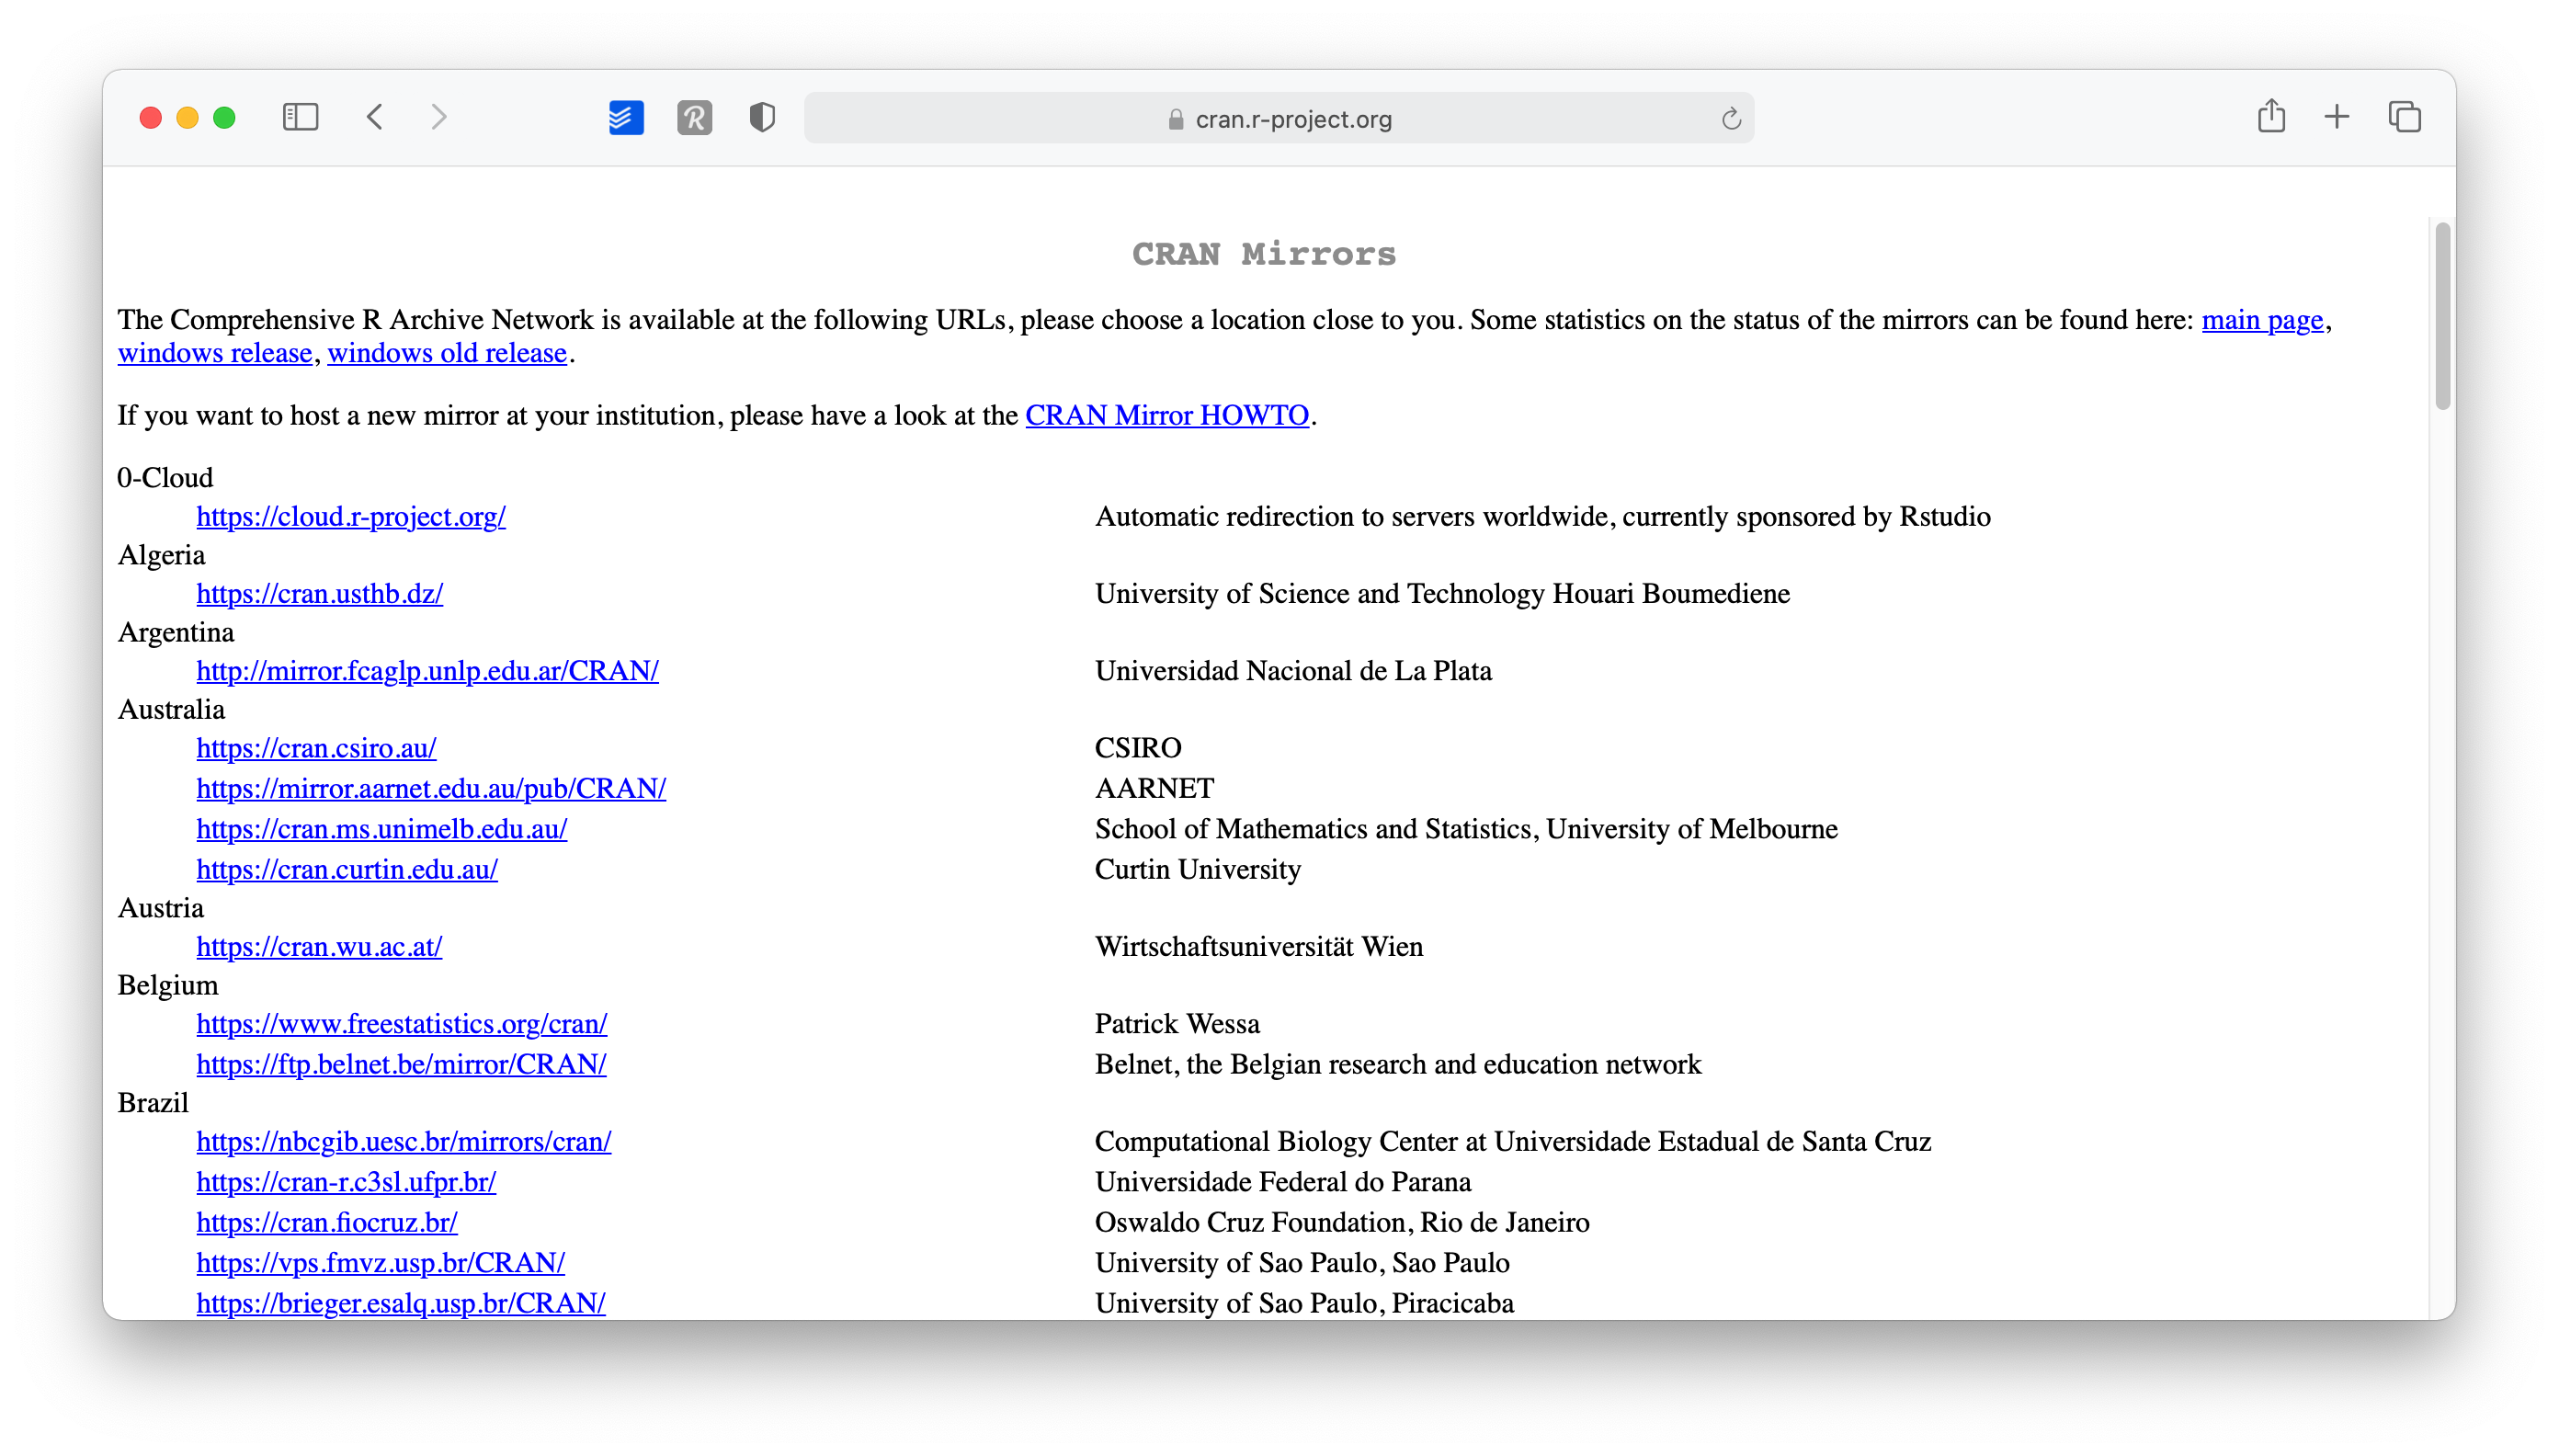
\includegraphics{images/chapter_03_img/r_project/01_r_project_cran_mirror.png}
\item
  Select the operating system for your computer.

  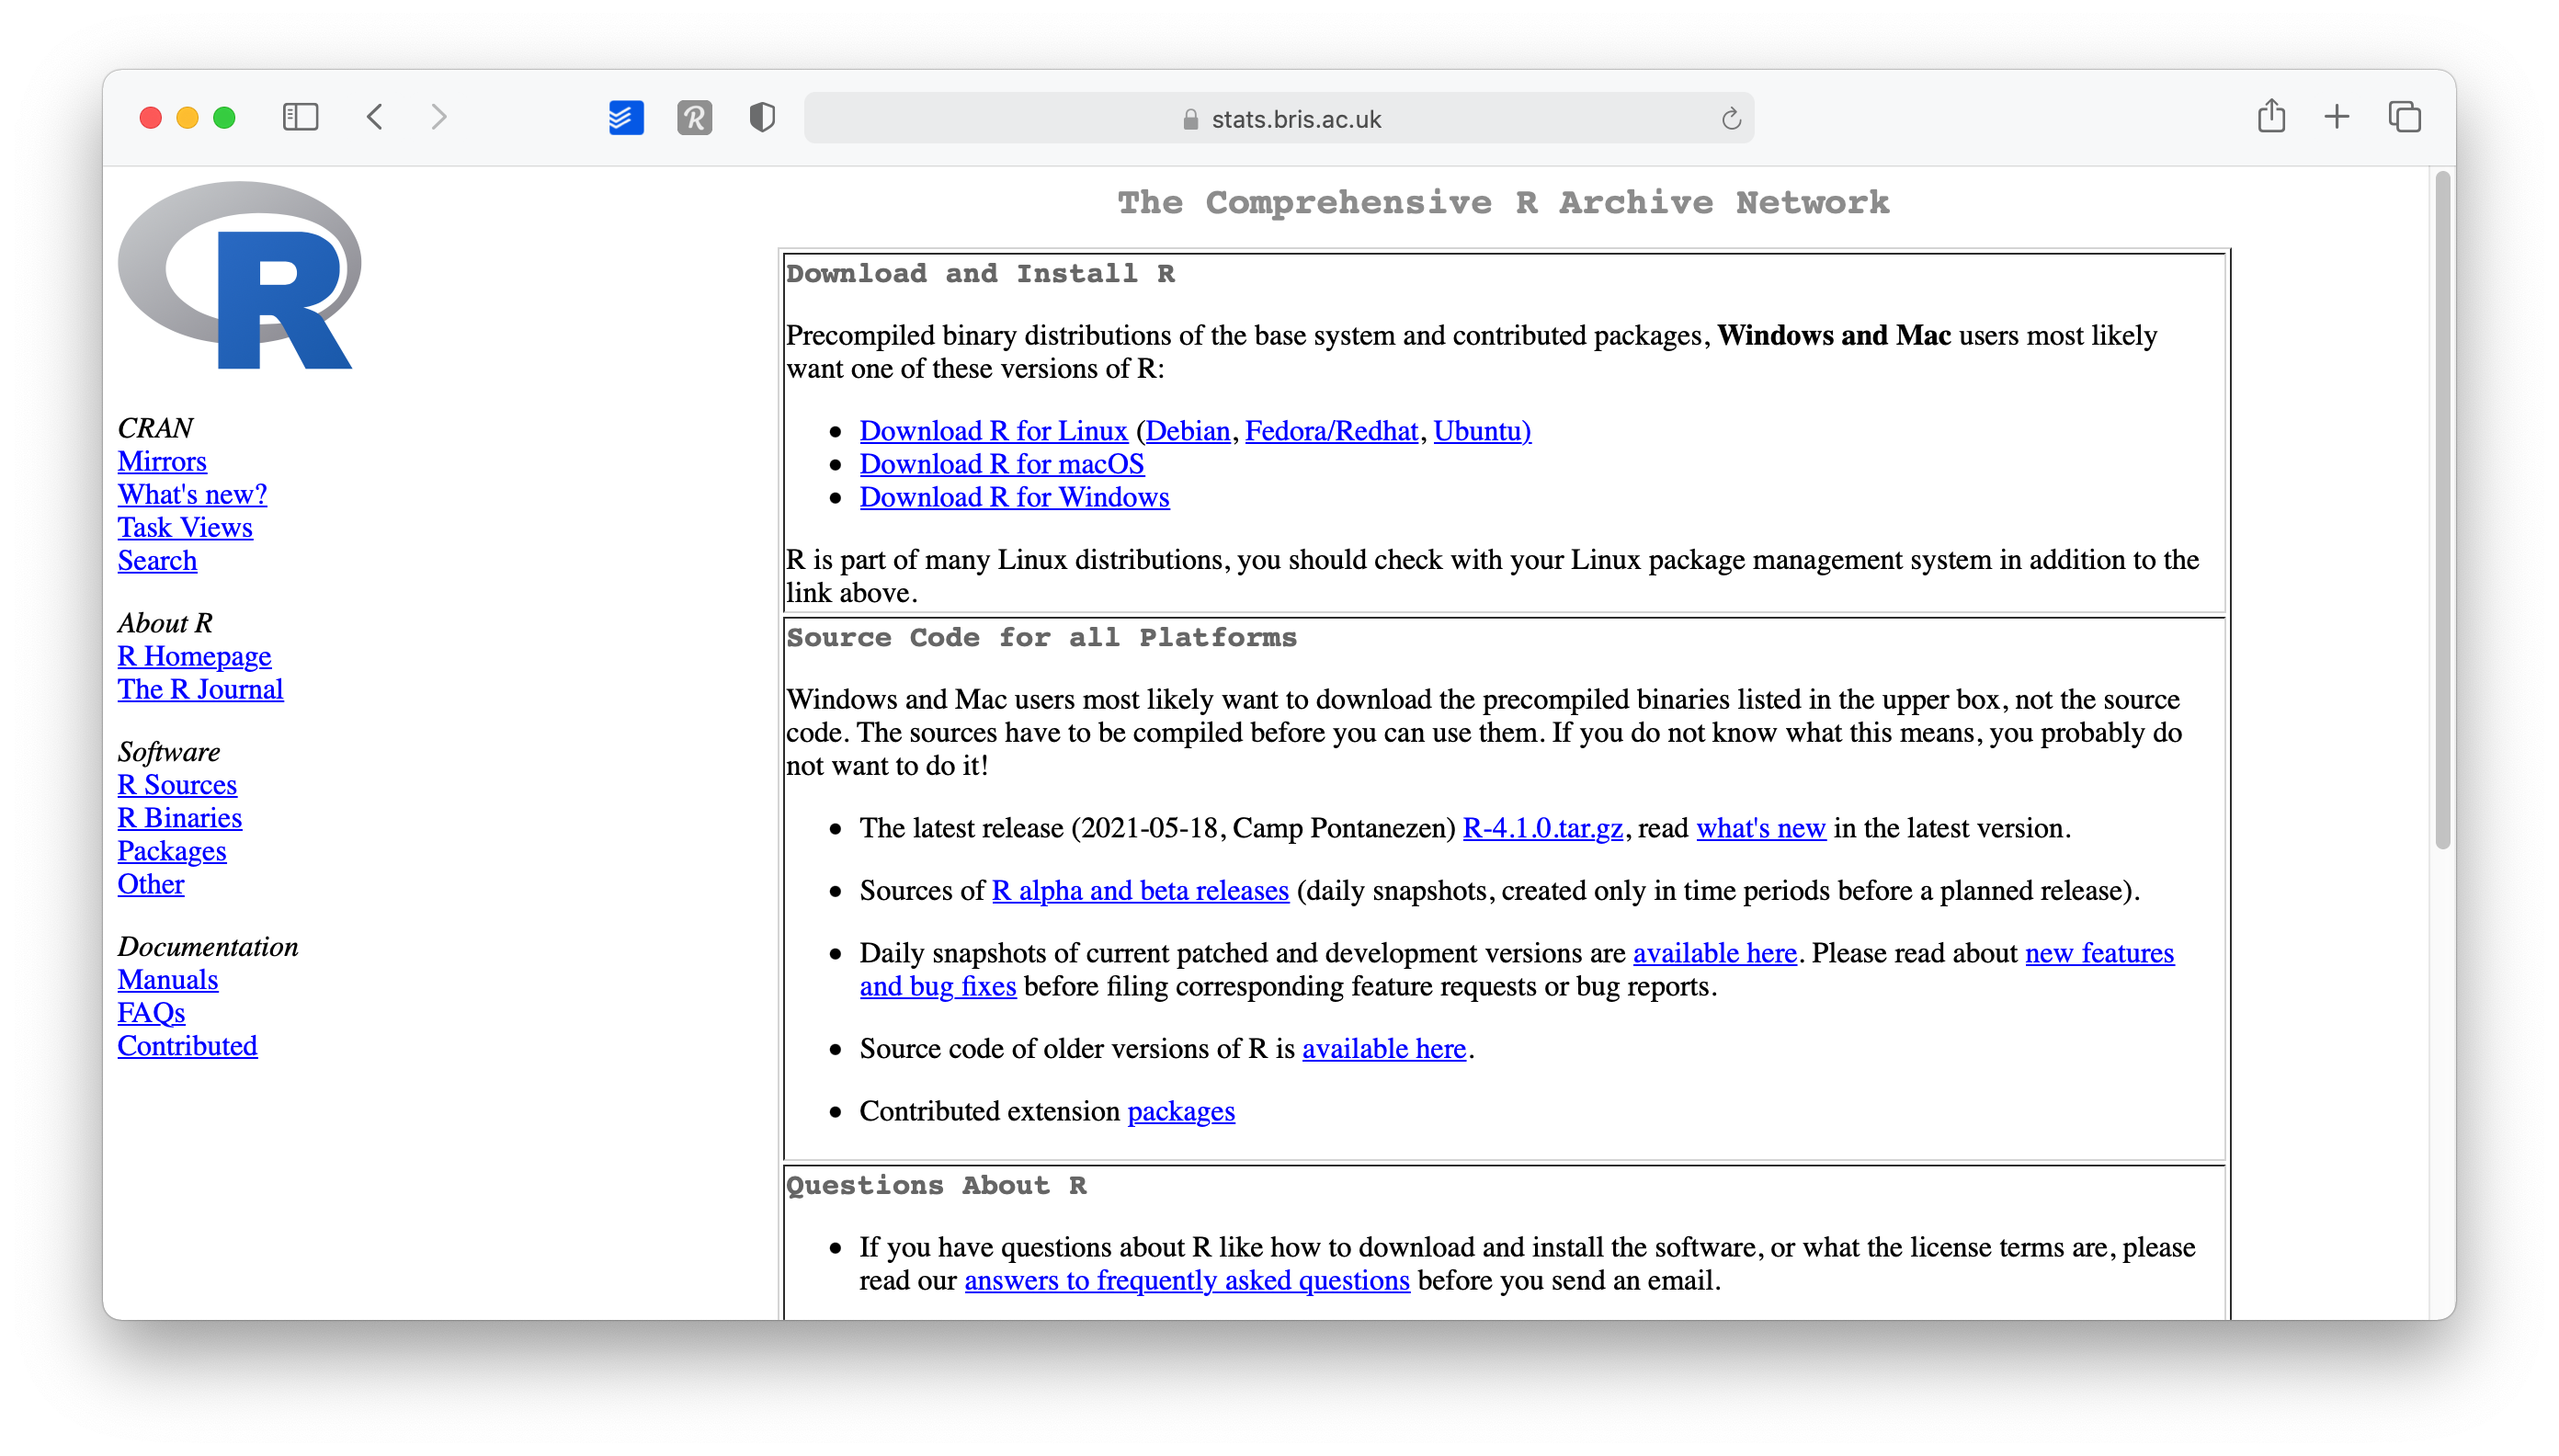
\includegraphics{images/chapter_03_img/r_project/02_r_project_os_choice.png}
\item
  Select the version you want to install (I recommend the latest version)

  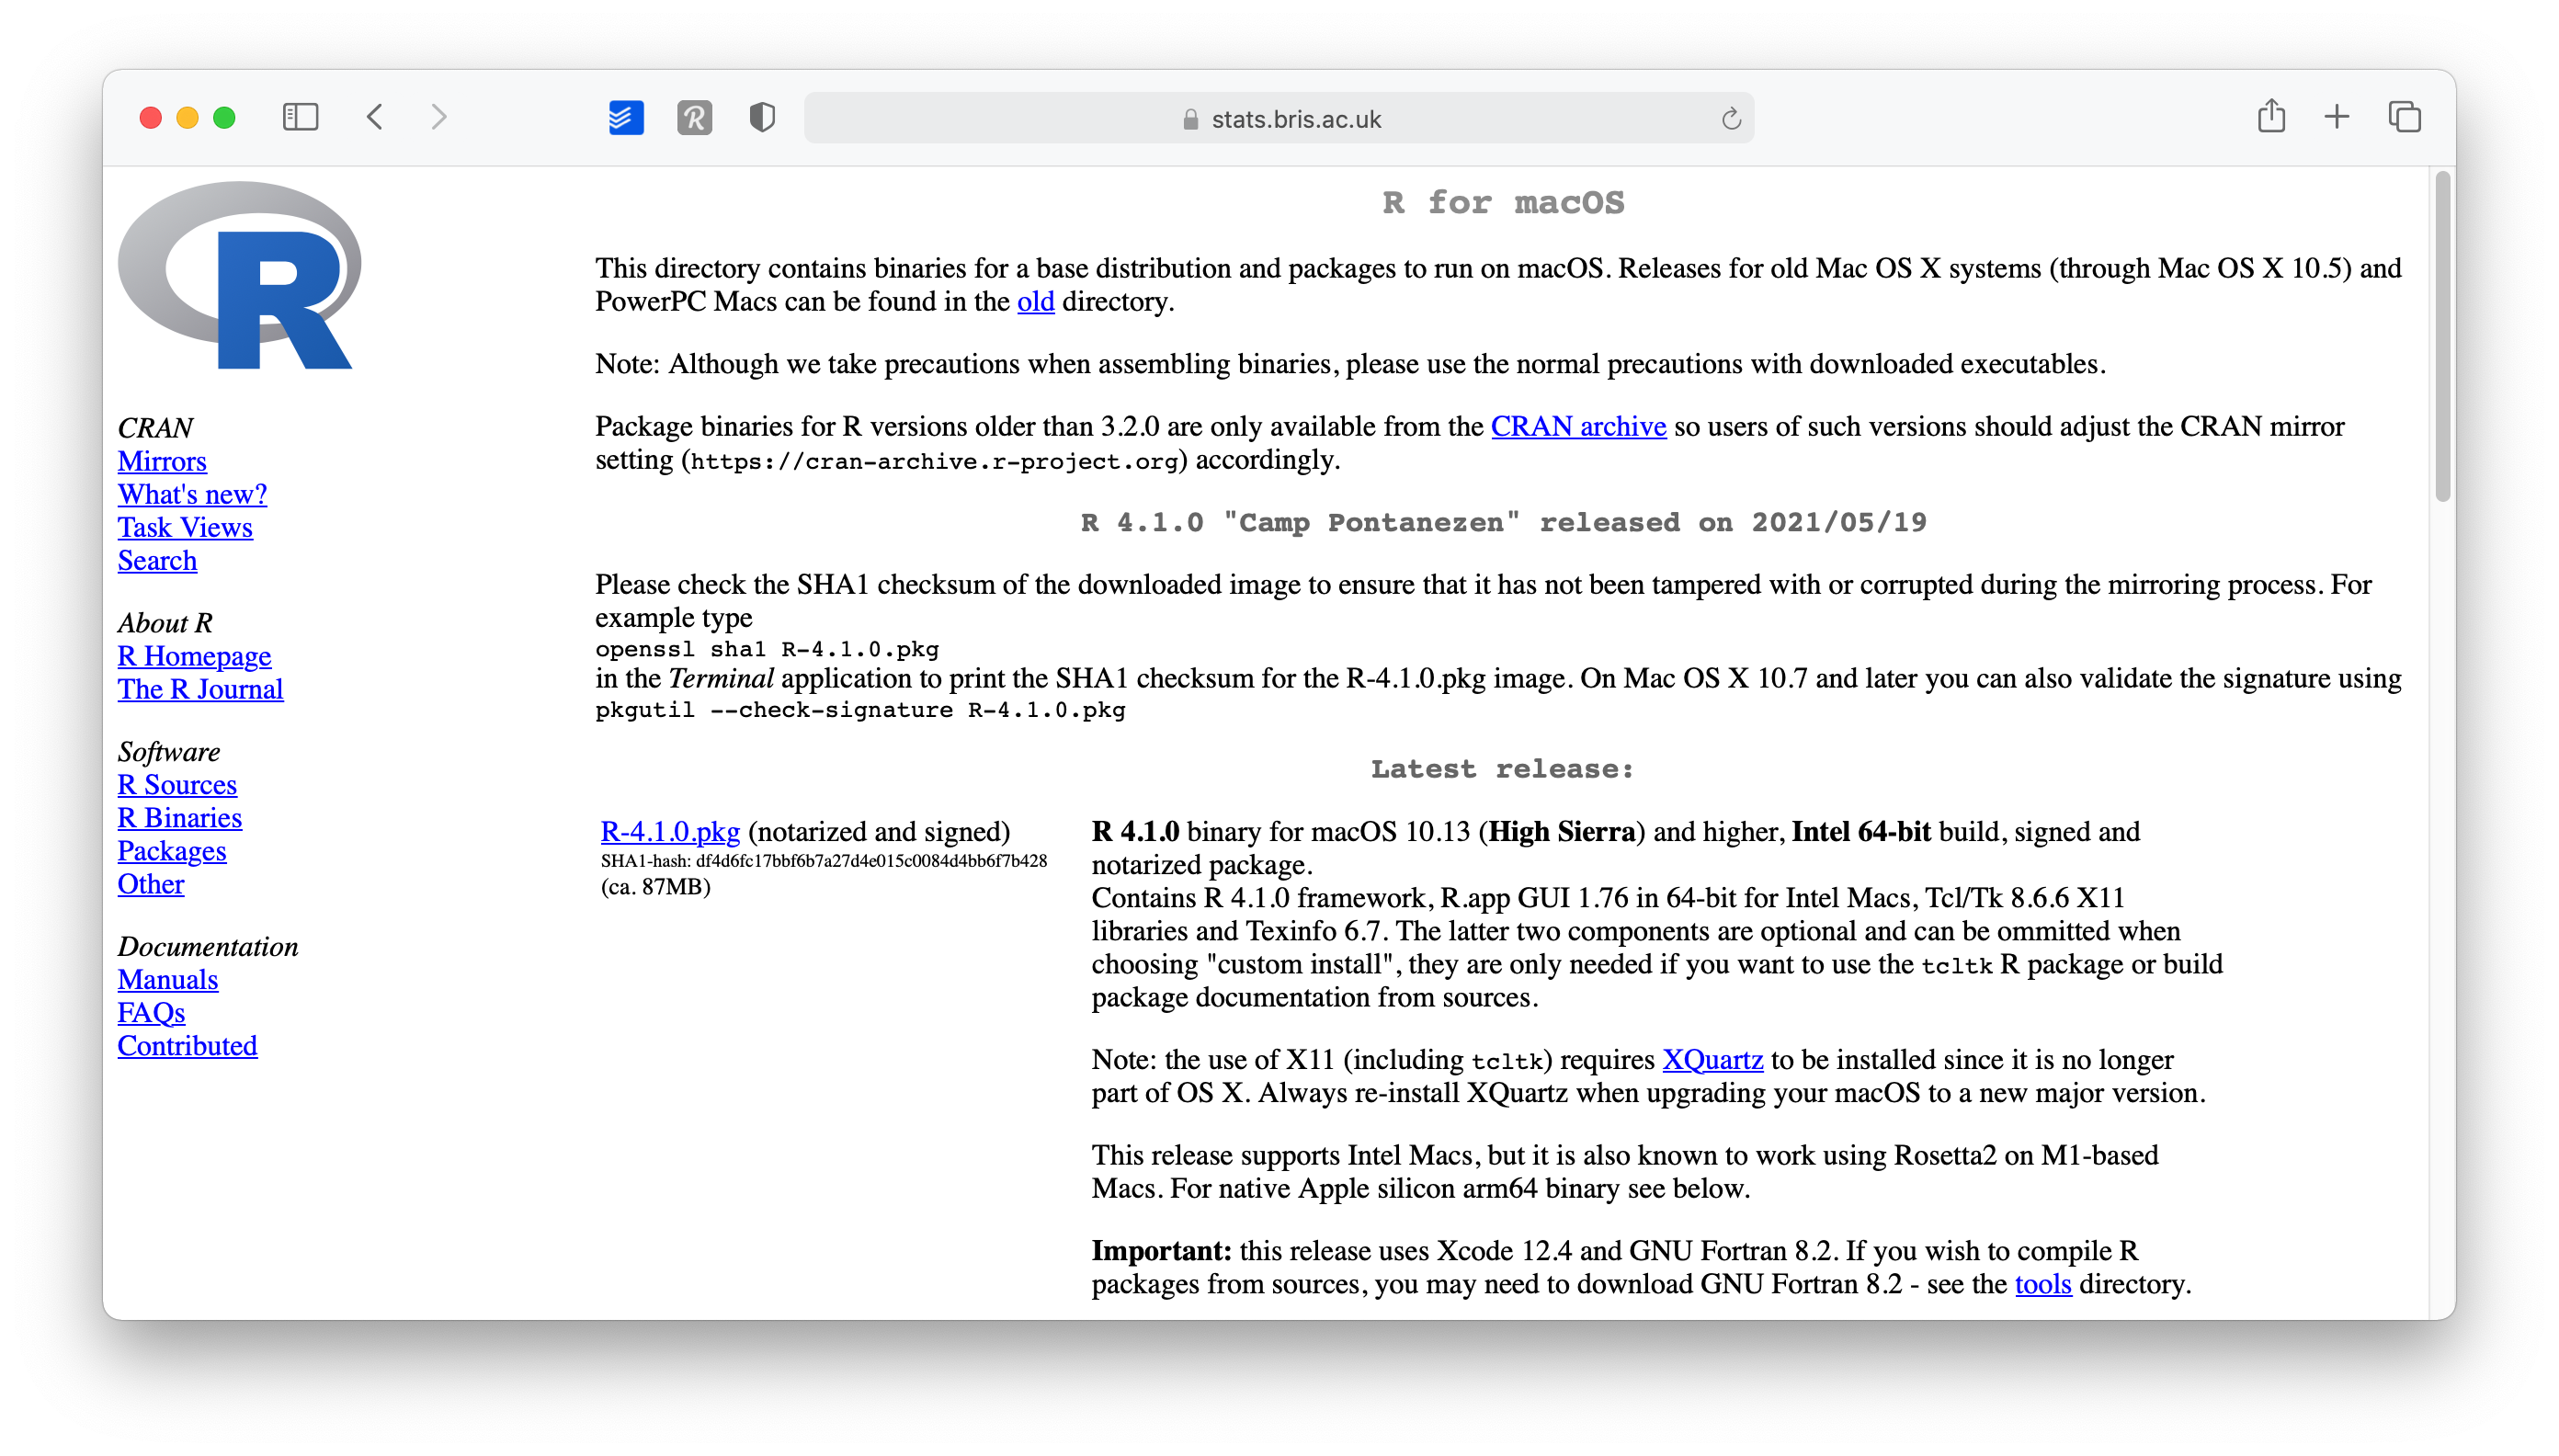
\includegraphics{images/chapter_03_img/r_project/03_r_project_version_choice.png}
\item
  Open the downloaded file and follow the installation instructions. (I recommend leaving the suggested settings as they are).
\end{enumerate}

This was relatively easy. You now have \emph{R} installed. Technically you can start using \emph{R} for your research, but there is one more tool I strongly advise installing: RStudio.

\hypertarget{installing-rstudio}{%
\section{Installing RStudio}\label{installing-rstudio}}

\emph{R} by itself is just the *`beating heart'* of \emph{R} programming, but it has no particular user interface. If you want buttons to click and actually `see' what you are doing, there is no better way than RStudio. RStudio is an \emph{integrated development environment} (IDE) and will be our primary tool to interact with \emph{R}. It is the only software you need to do all the fun parts and, of course, to follow along with the examples of this book. To install RStudio perform the following steps:

\begin{enumerate}
\def\labelenumi{\arabic{enumi}.}
\item
  Go to \href{https://www.rstudio.com\%5D(https://www.rstudio.com)}{www.rstudio.com}.

  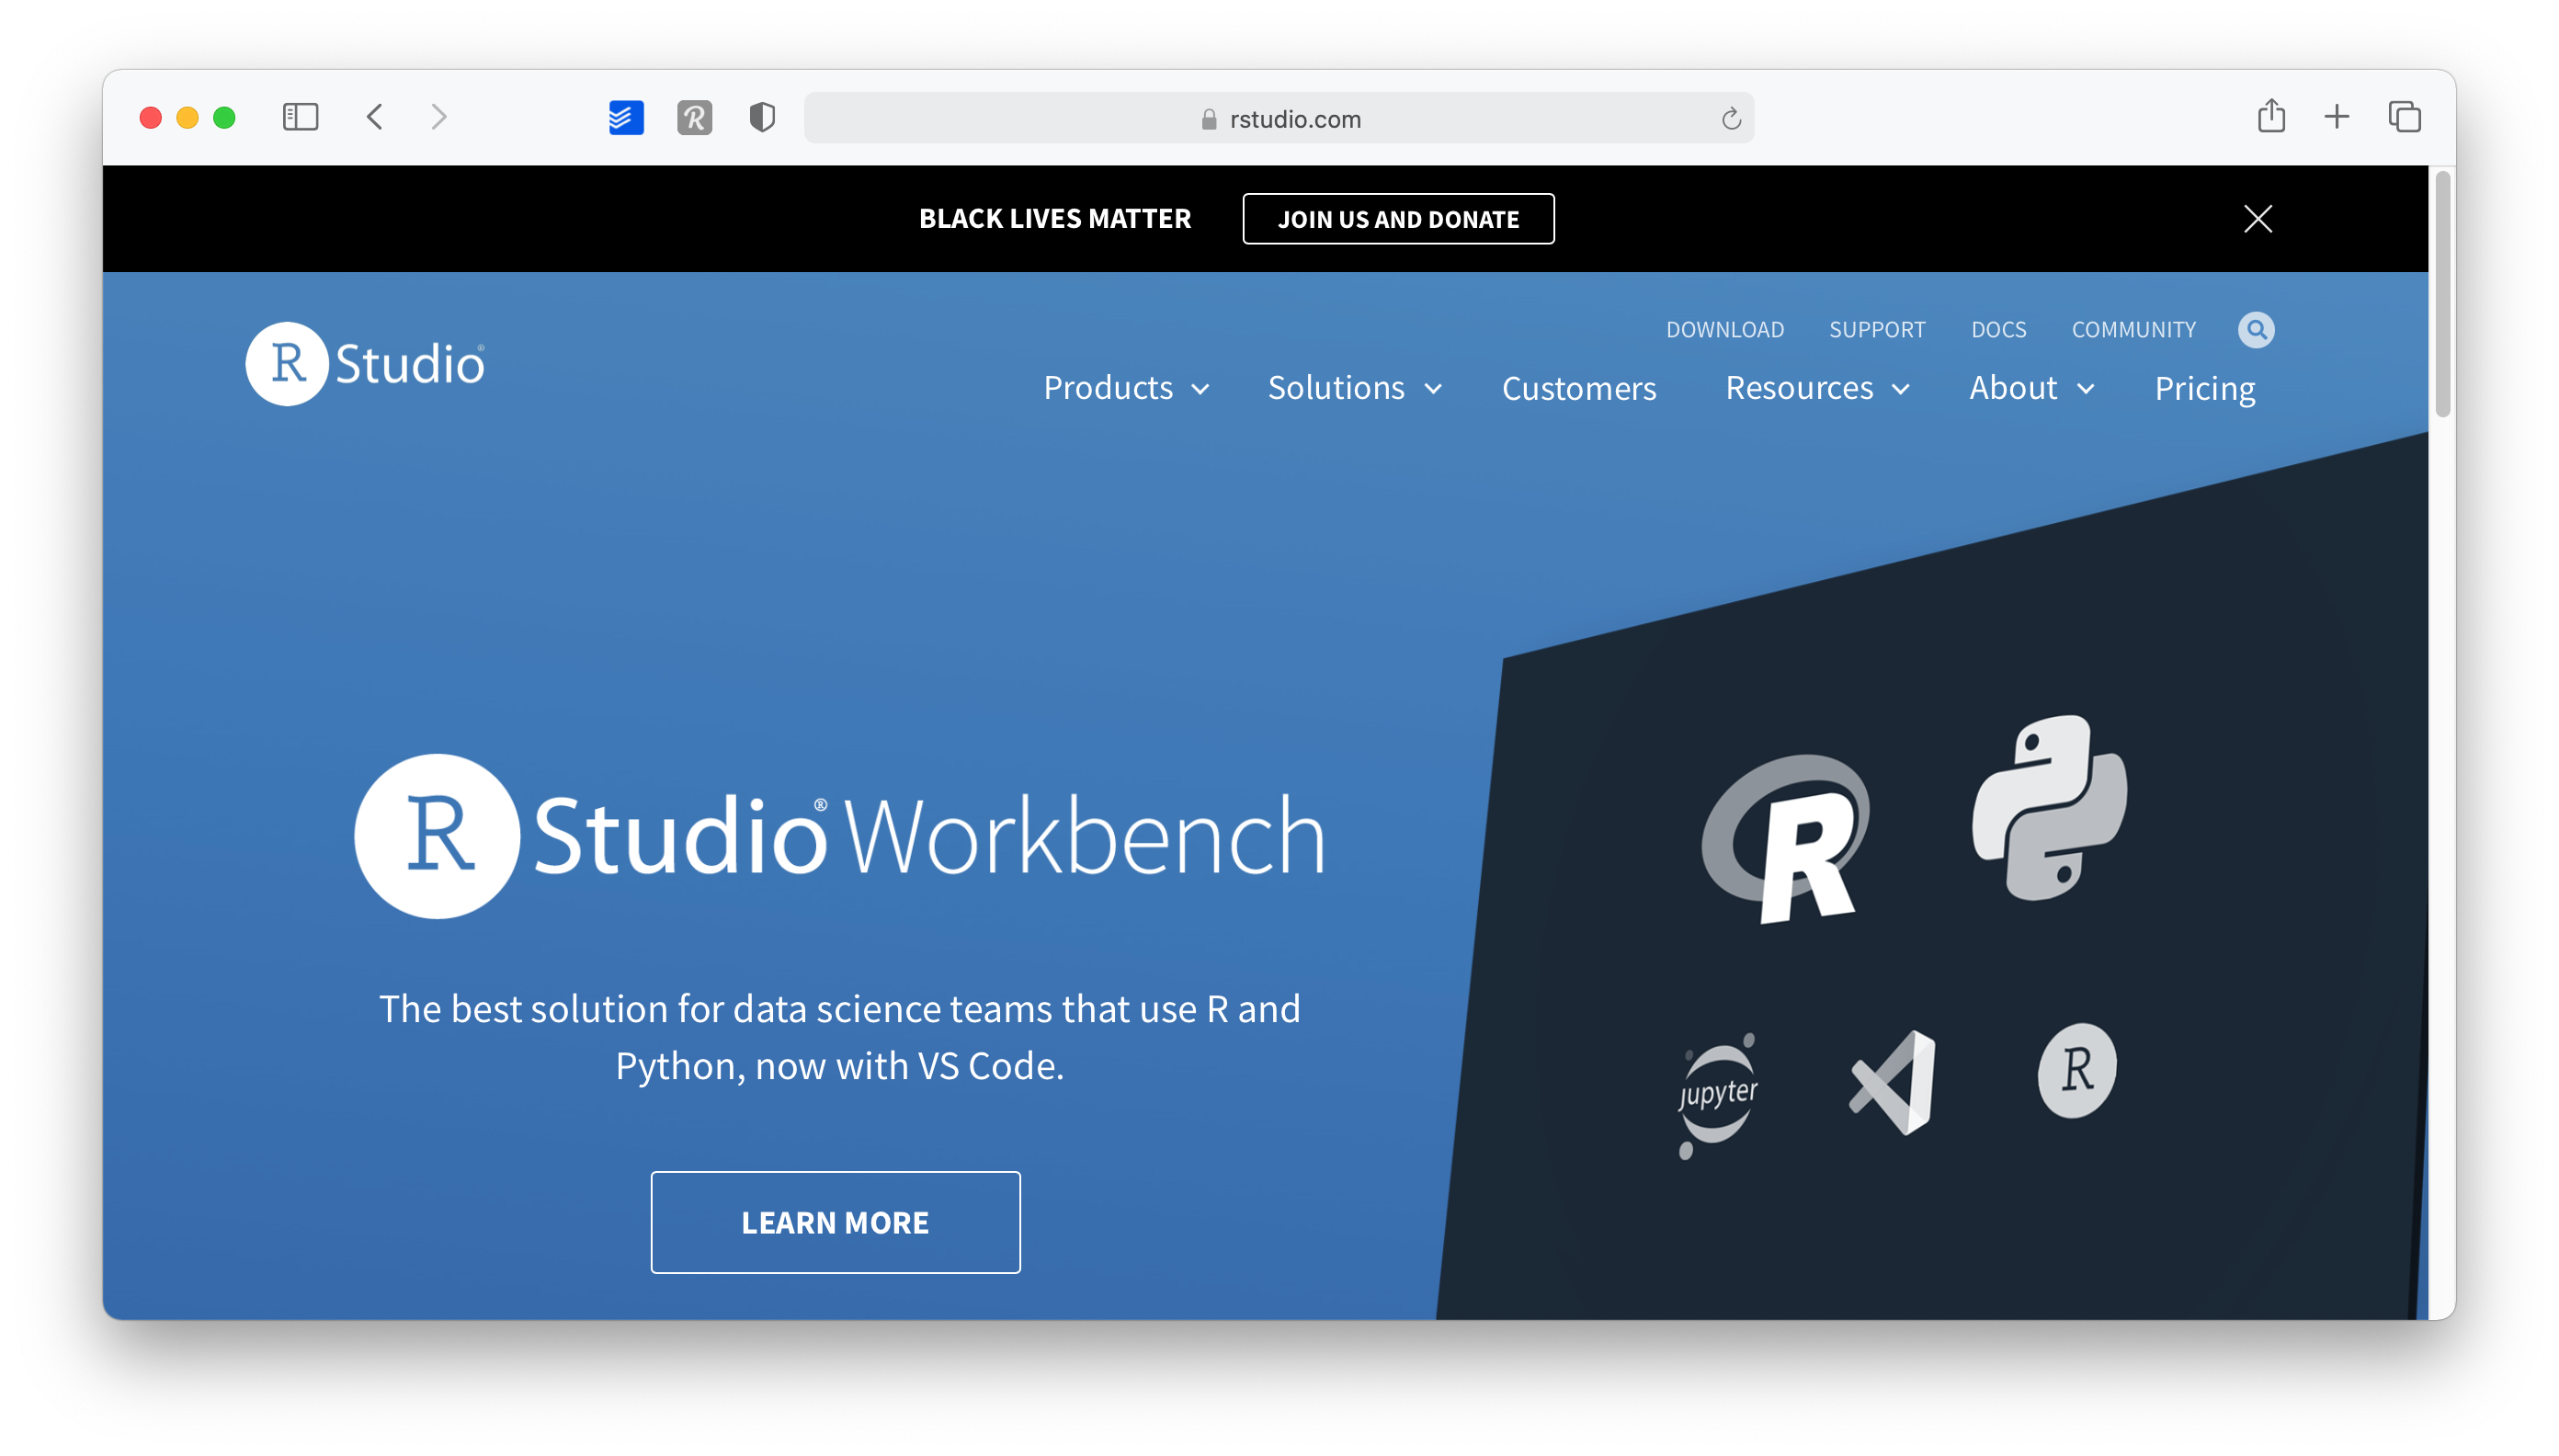
\includegraphics{images/chapter_03_img/rstudio/01_rstudio_main_page.png}
\item
  Go to \texttt{Products\ \textgreater{}\ RStudio}

  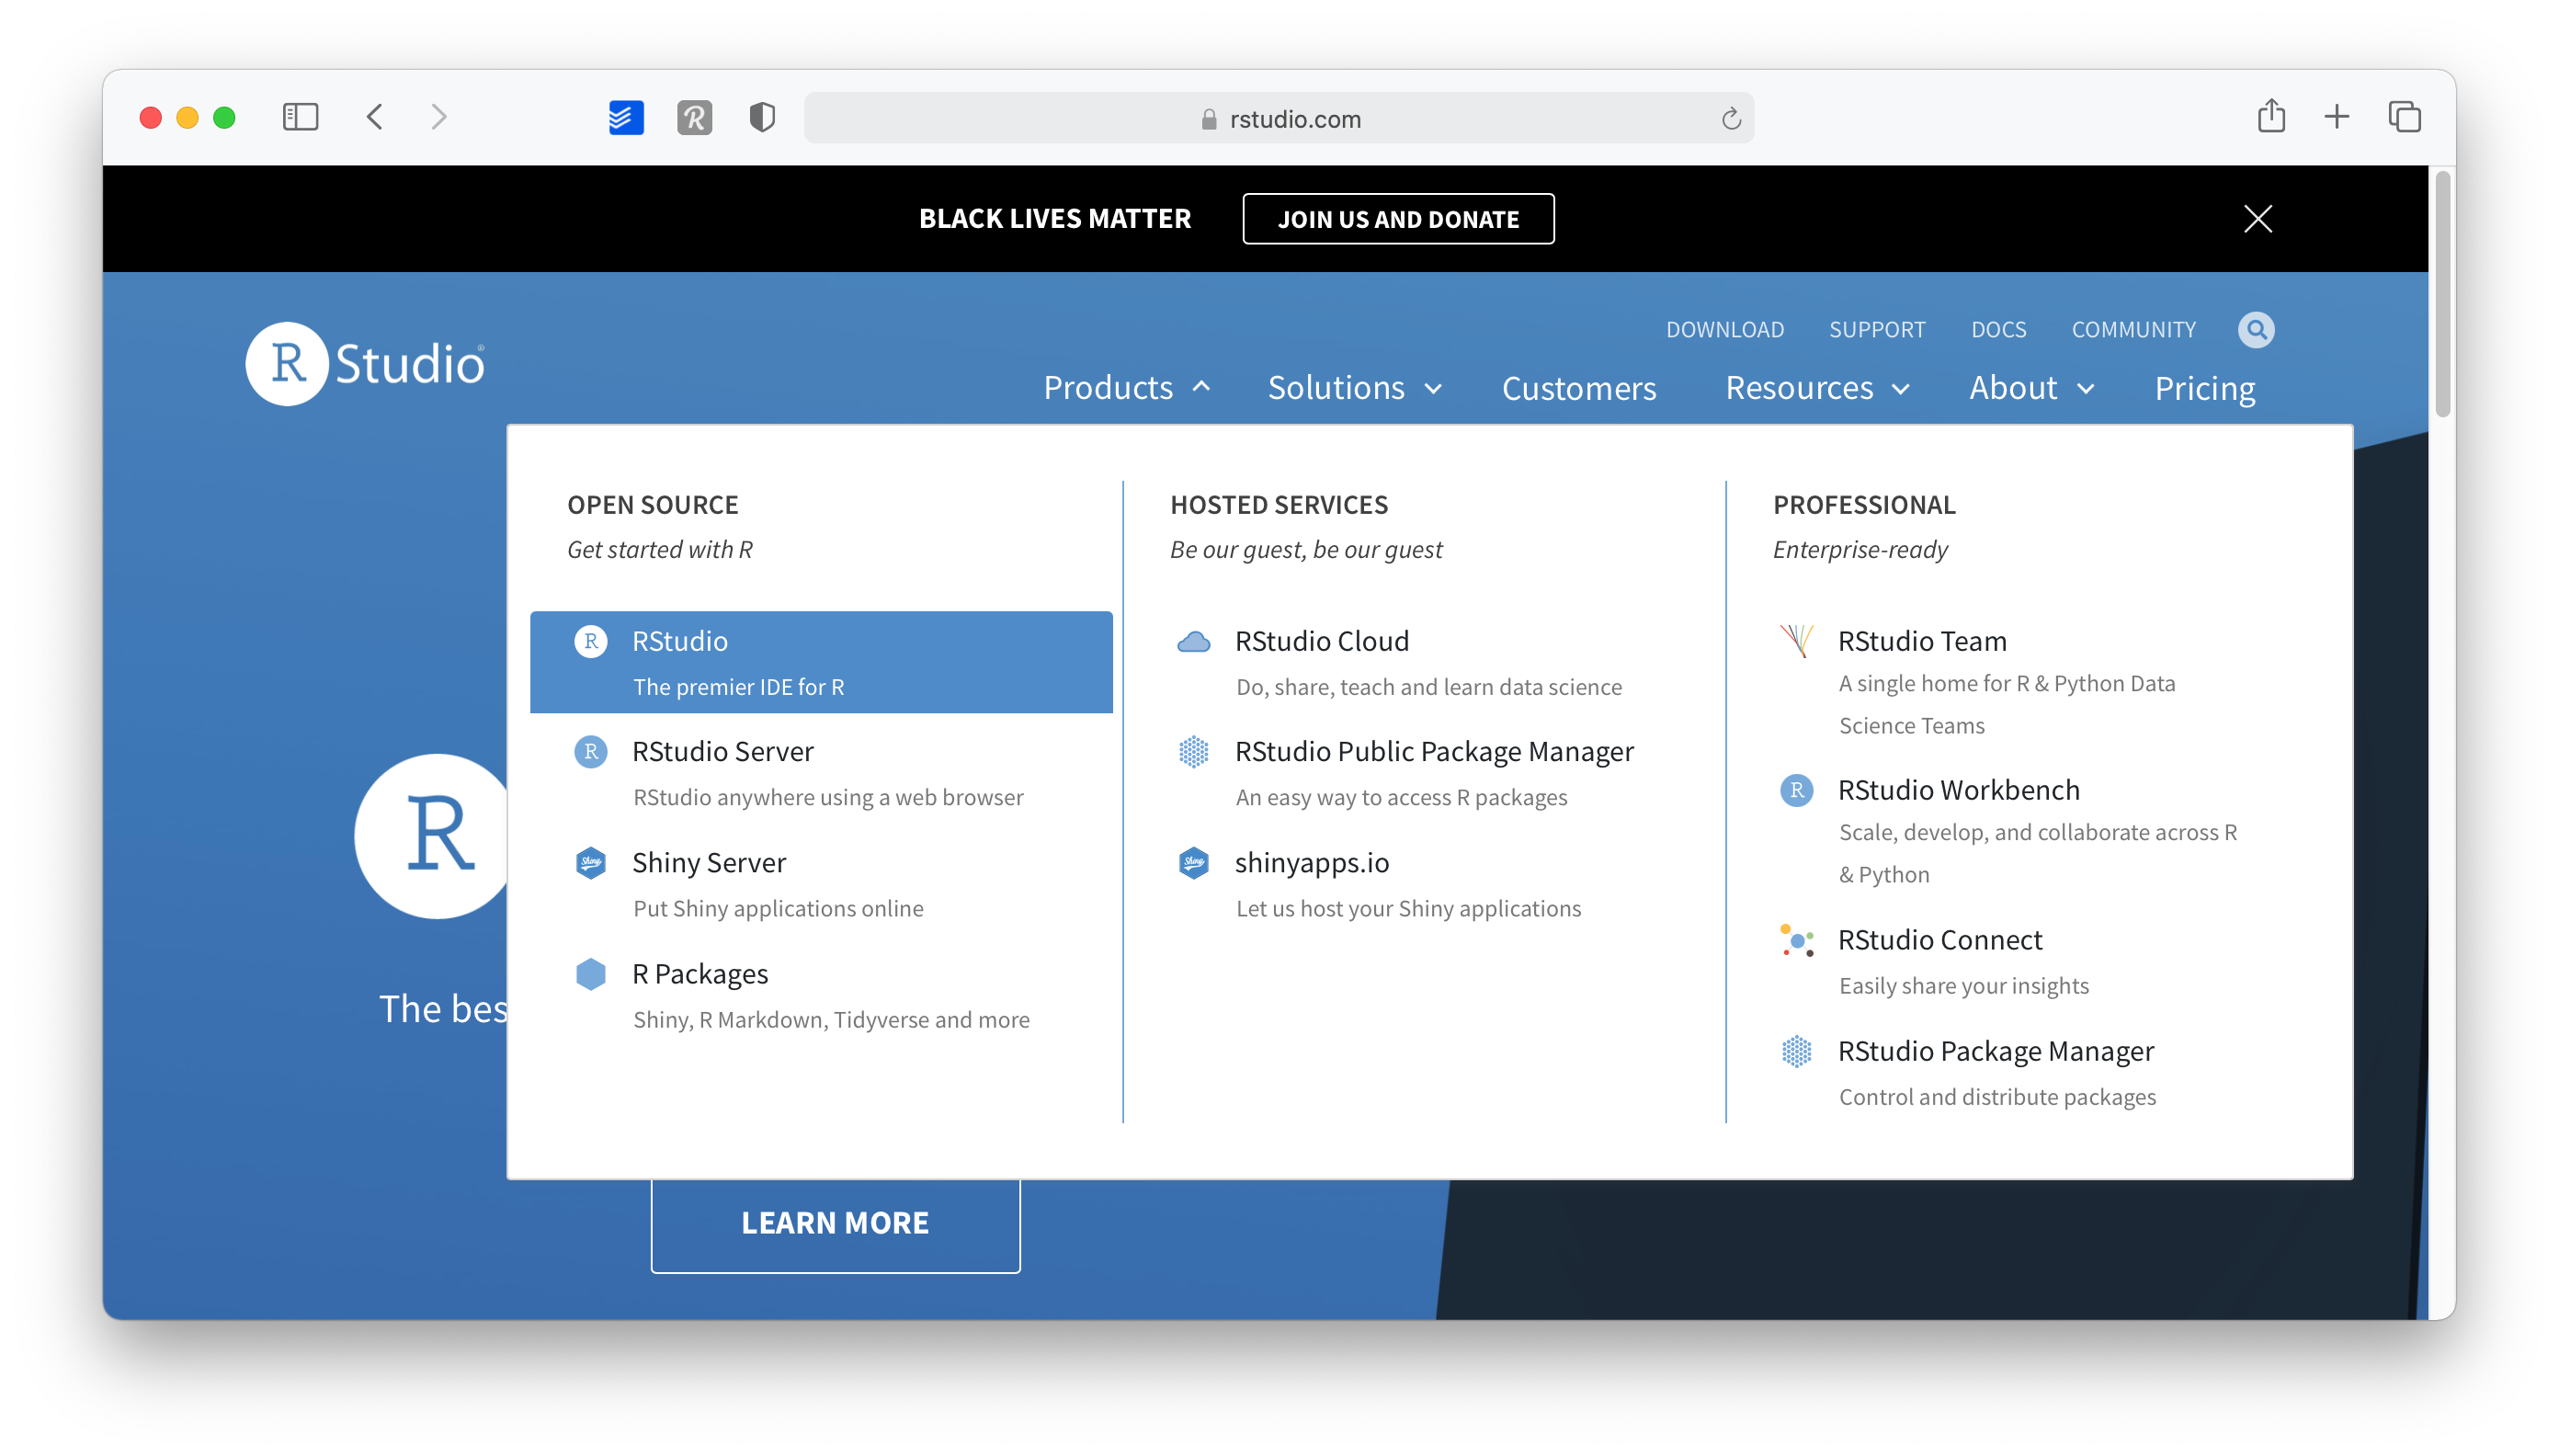
\includegraphics{images/chapter_03_img/rstudio/02_rstudio_main_page_menu.png}
\item
  On this page, scroll down and select \texttt{RStudio\ Desktop}

  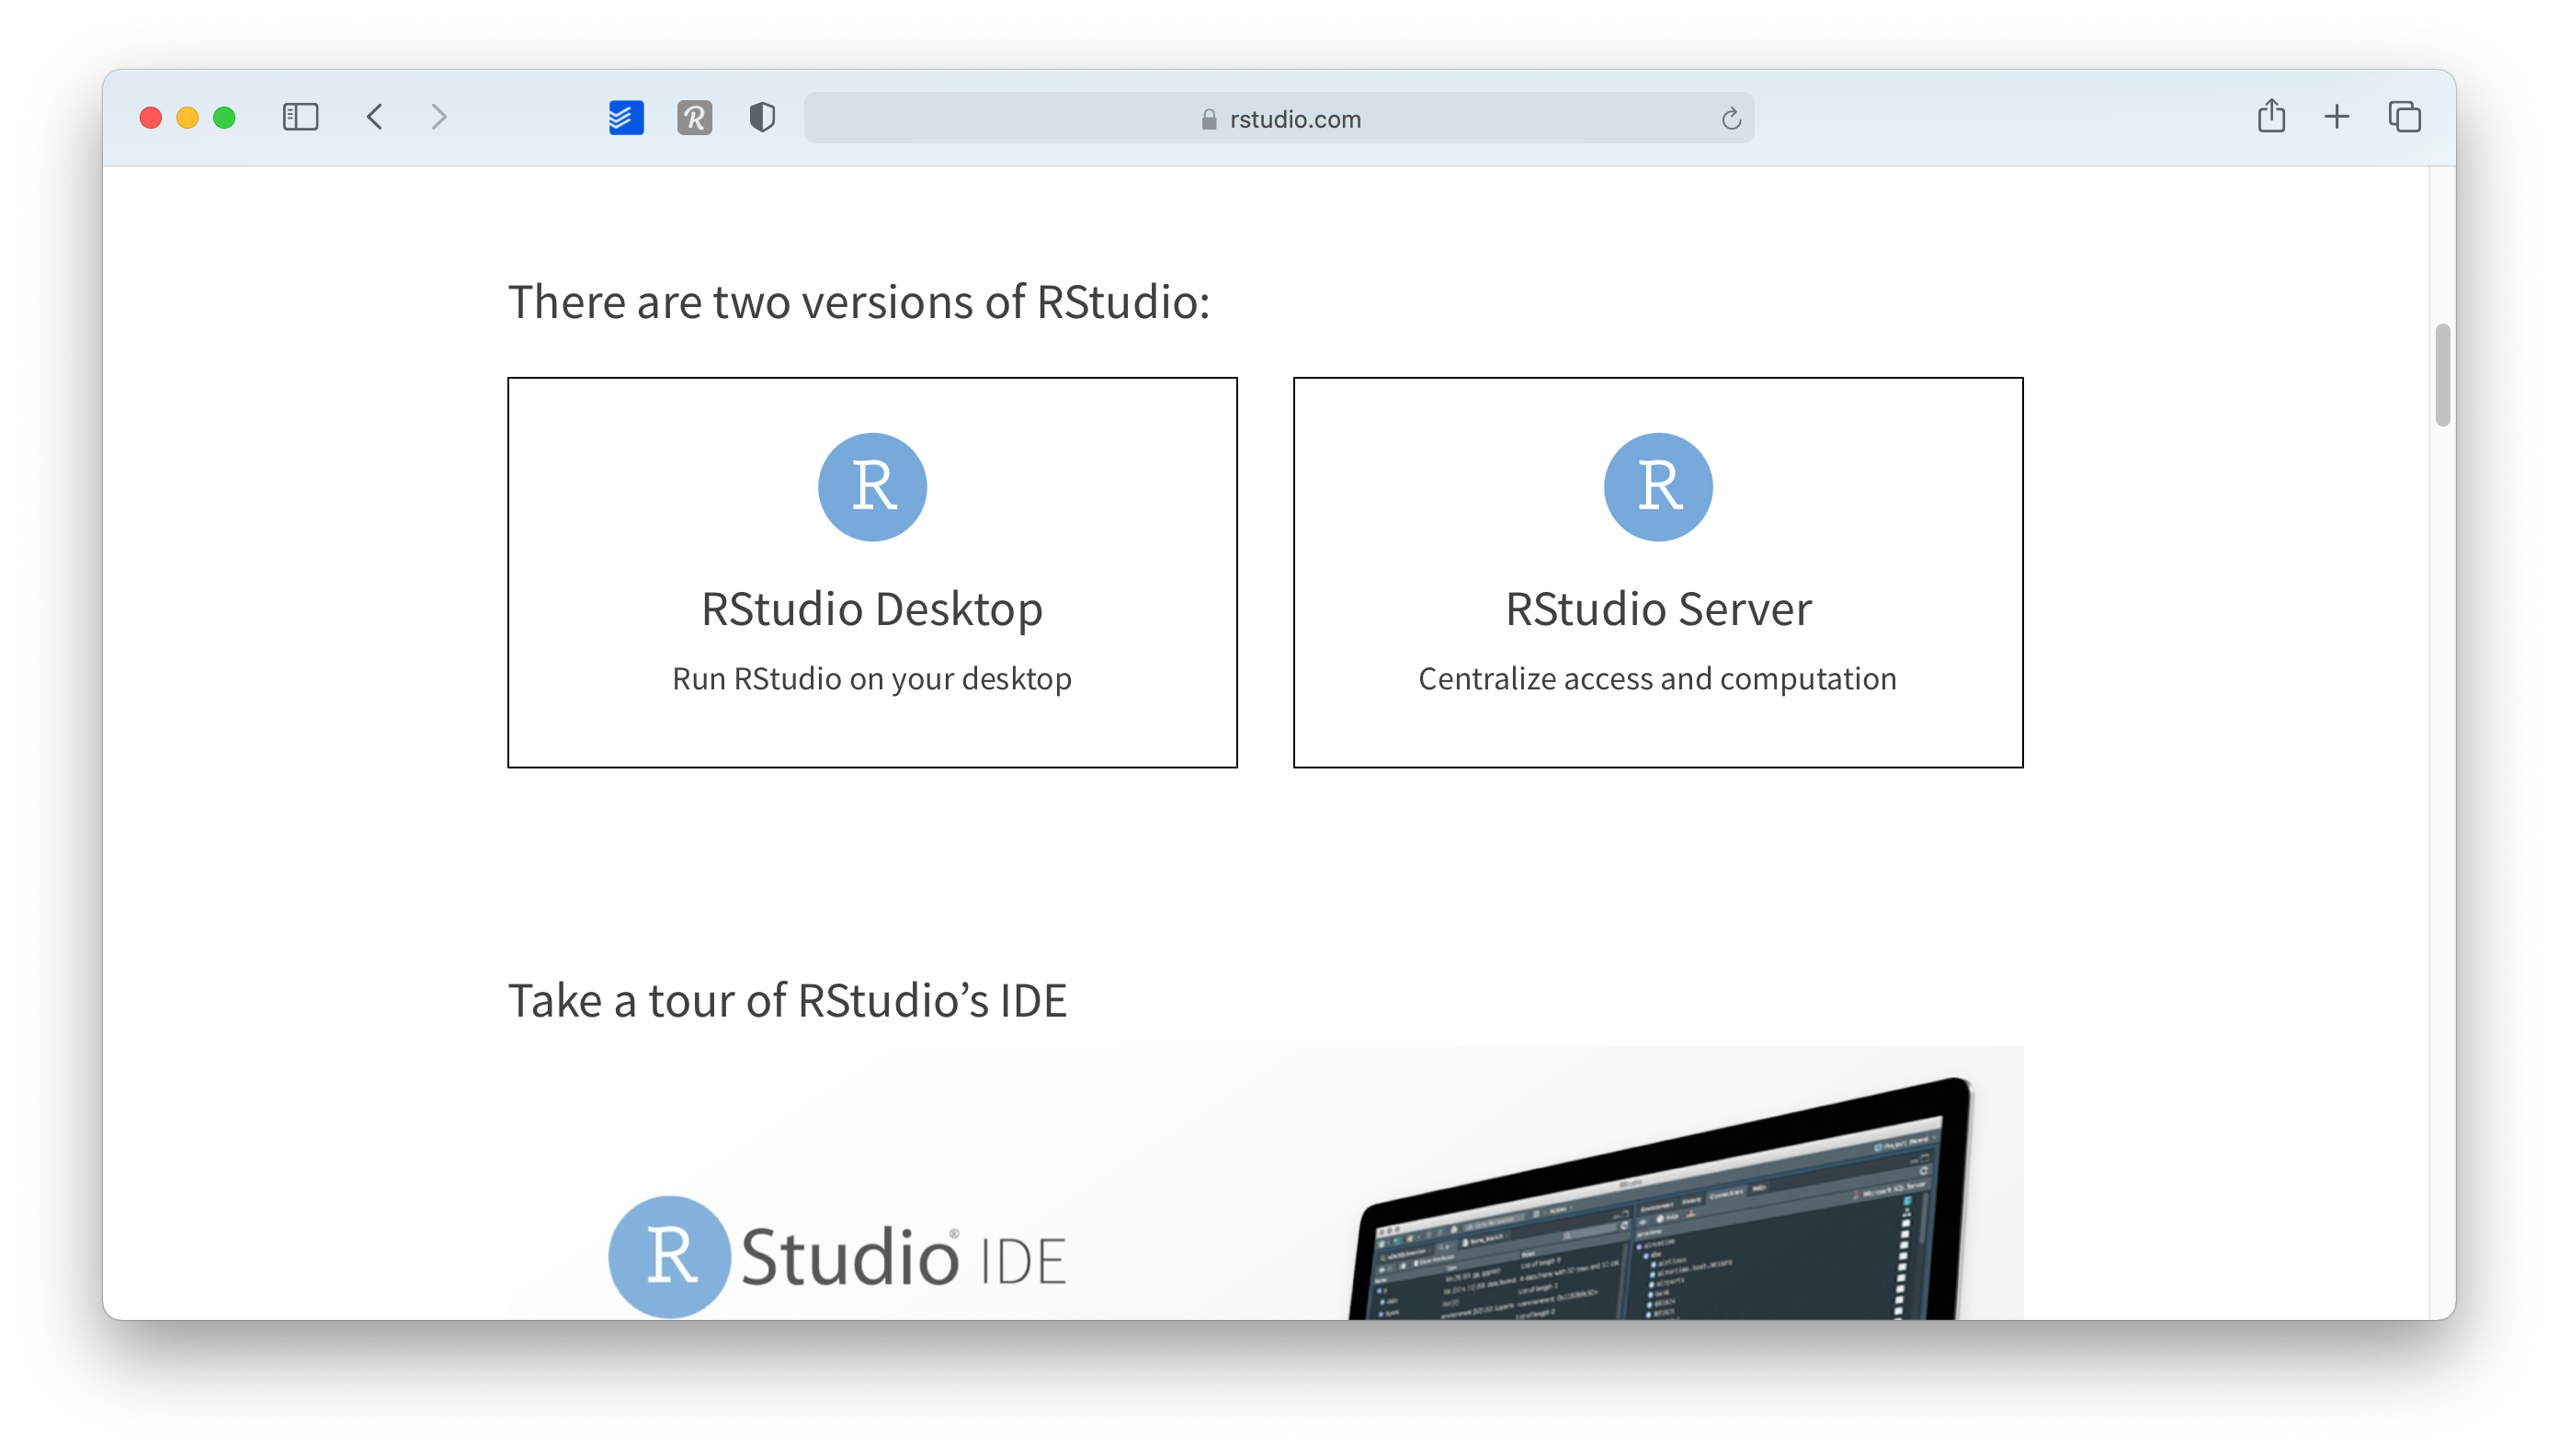
\includegraphics{images/chapter_03_img/rstudio/03_rstudio_select_version.png}
\item
  Select the \texttt{\textquotesingle{}Open\ Source\ Edition\textquotesingle{}} option by clicking on '\texttt{Download\ RStudio\ Desktop\textquotesingle{}}

  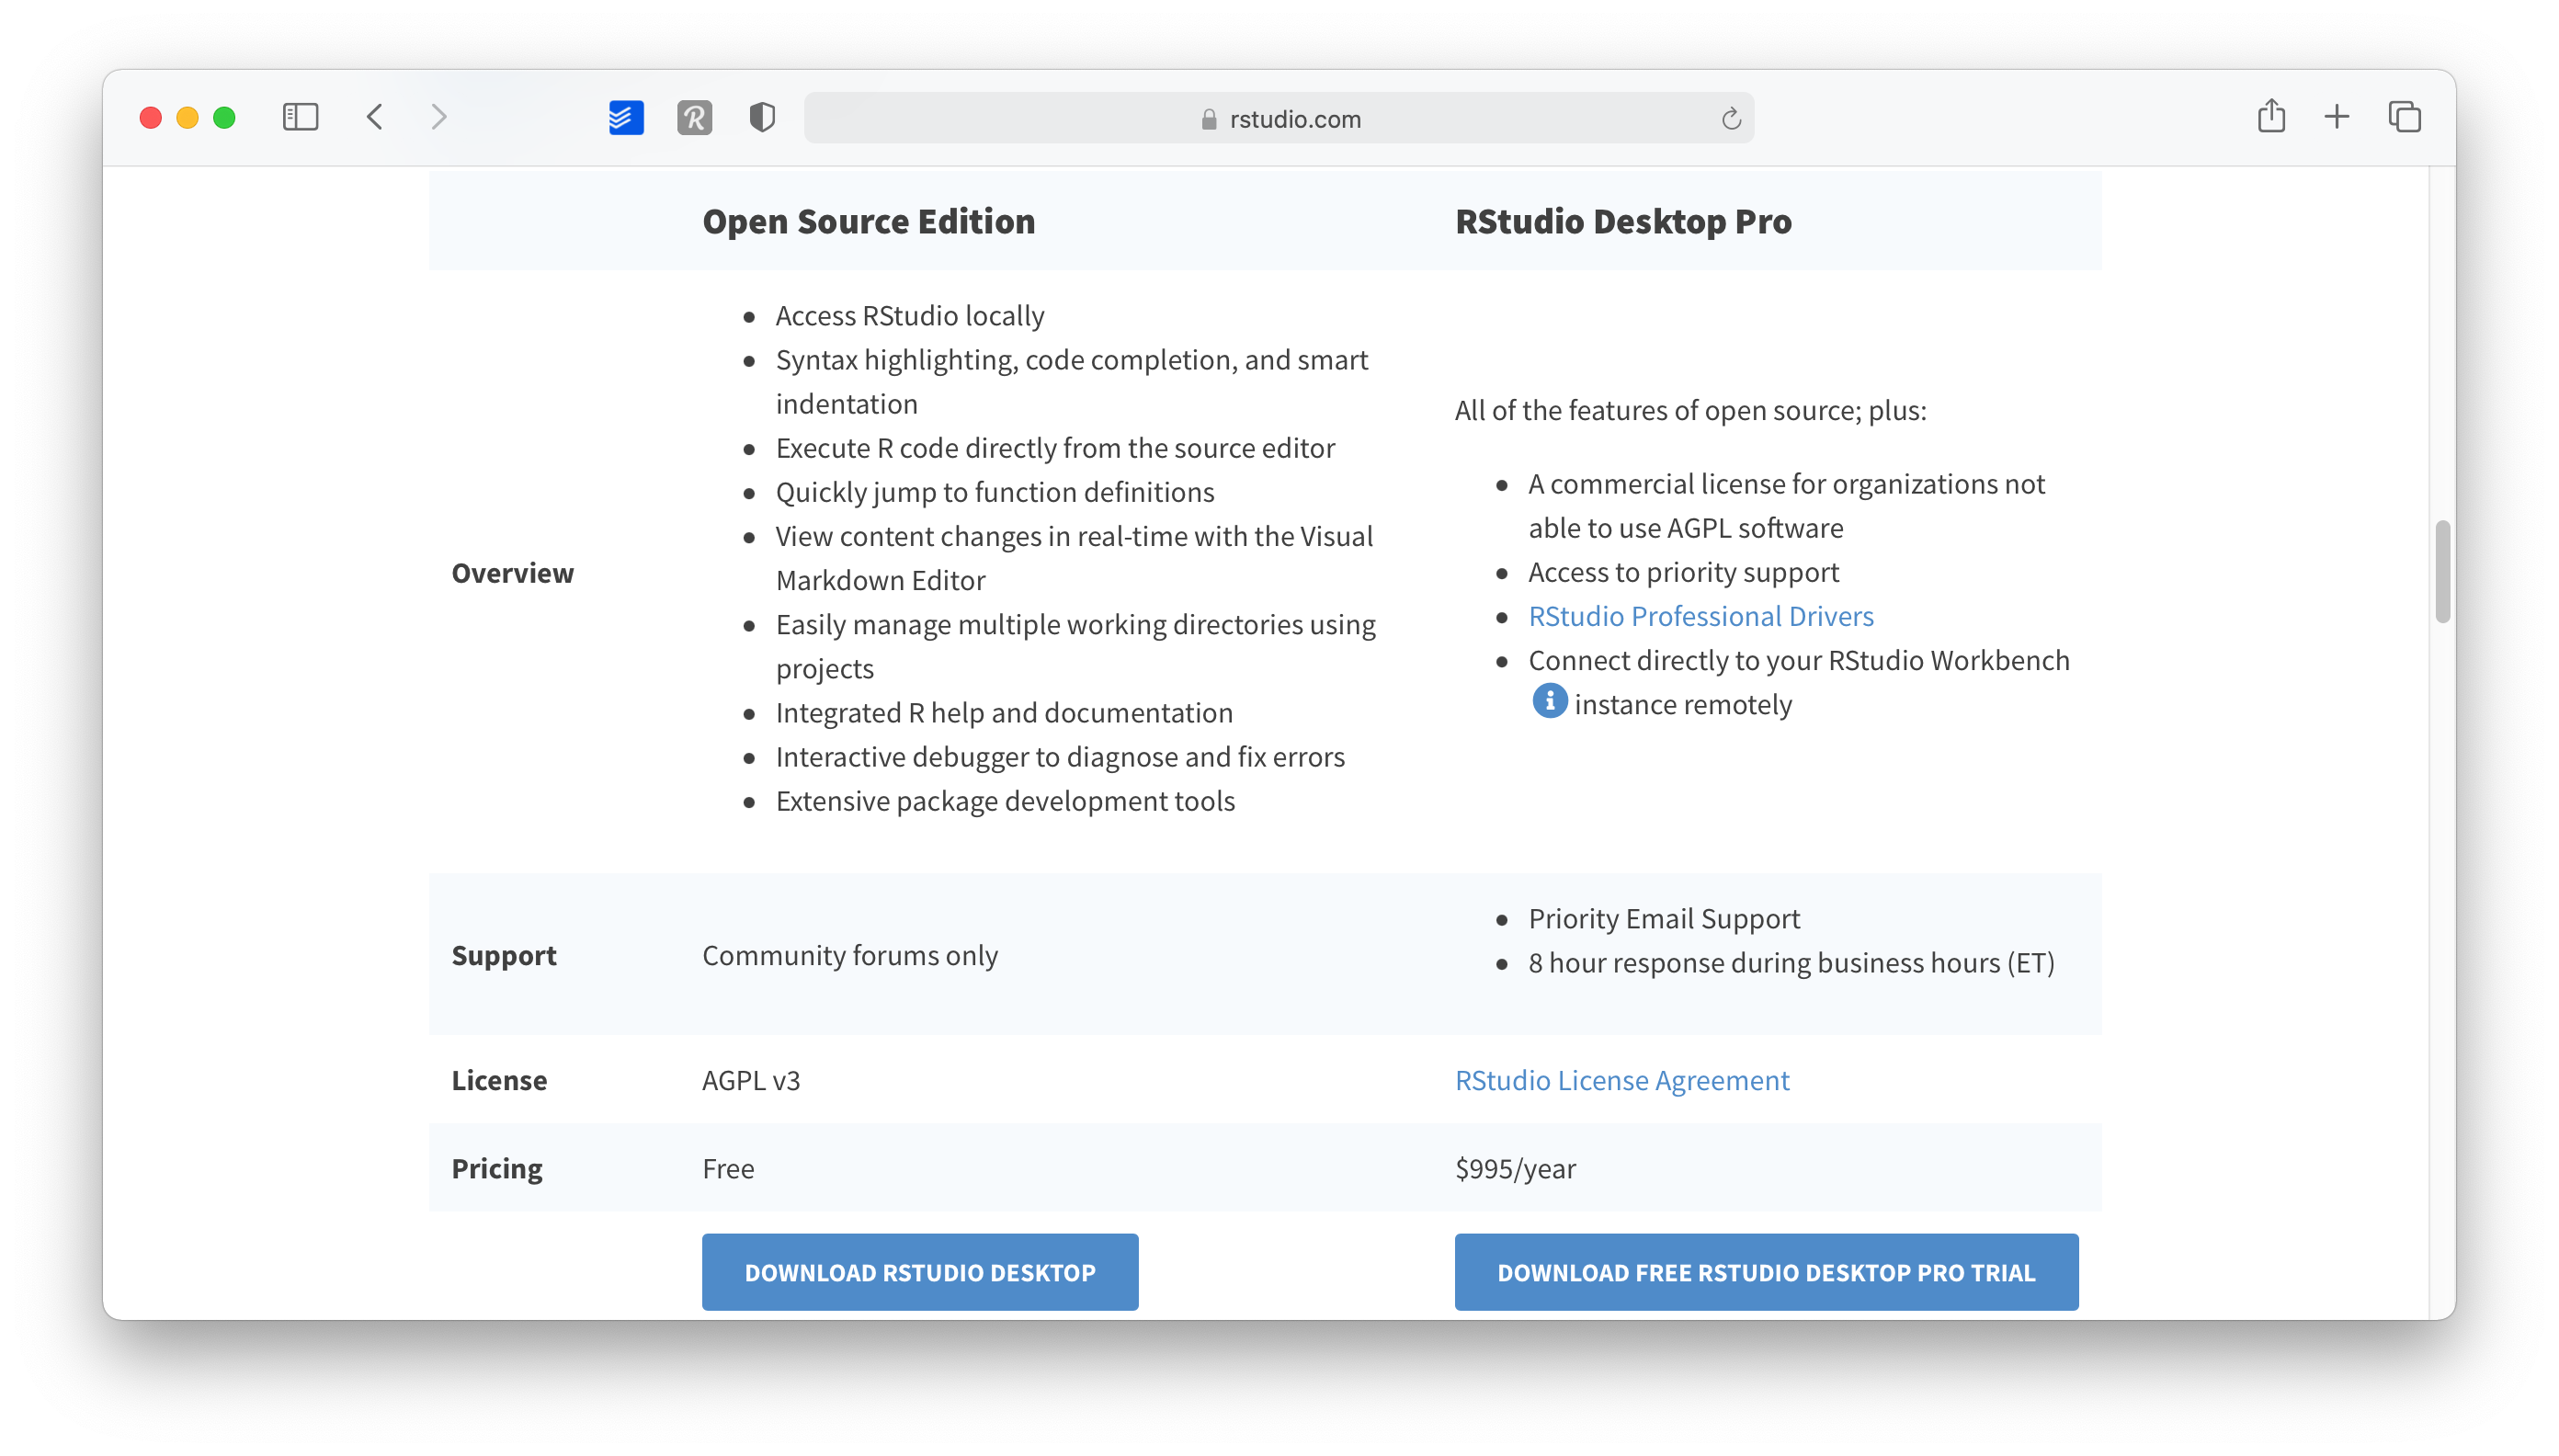
\includegraphics{images/chapter_03_img/rstudio/04_rstudio_select_edition.png}
\item
  As a last step, scroll down where it shows you a download button for your operating system. The website will automatically detect this. You also get a nice reminder to install `R' first, in case you have not done so yet.

  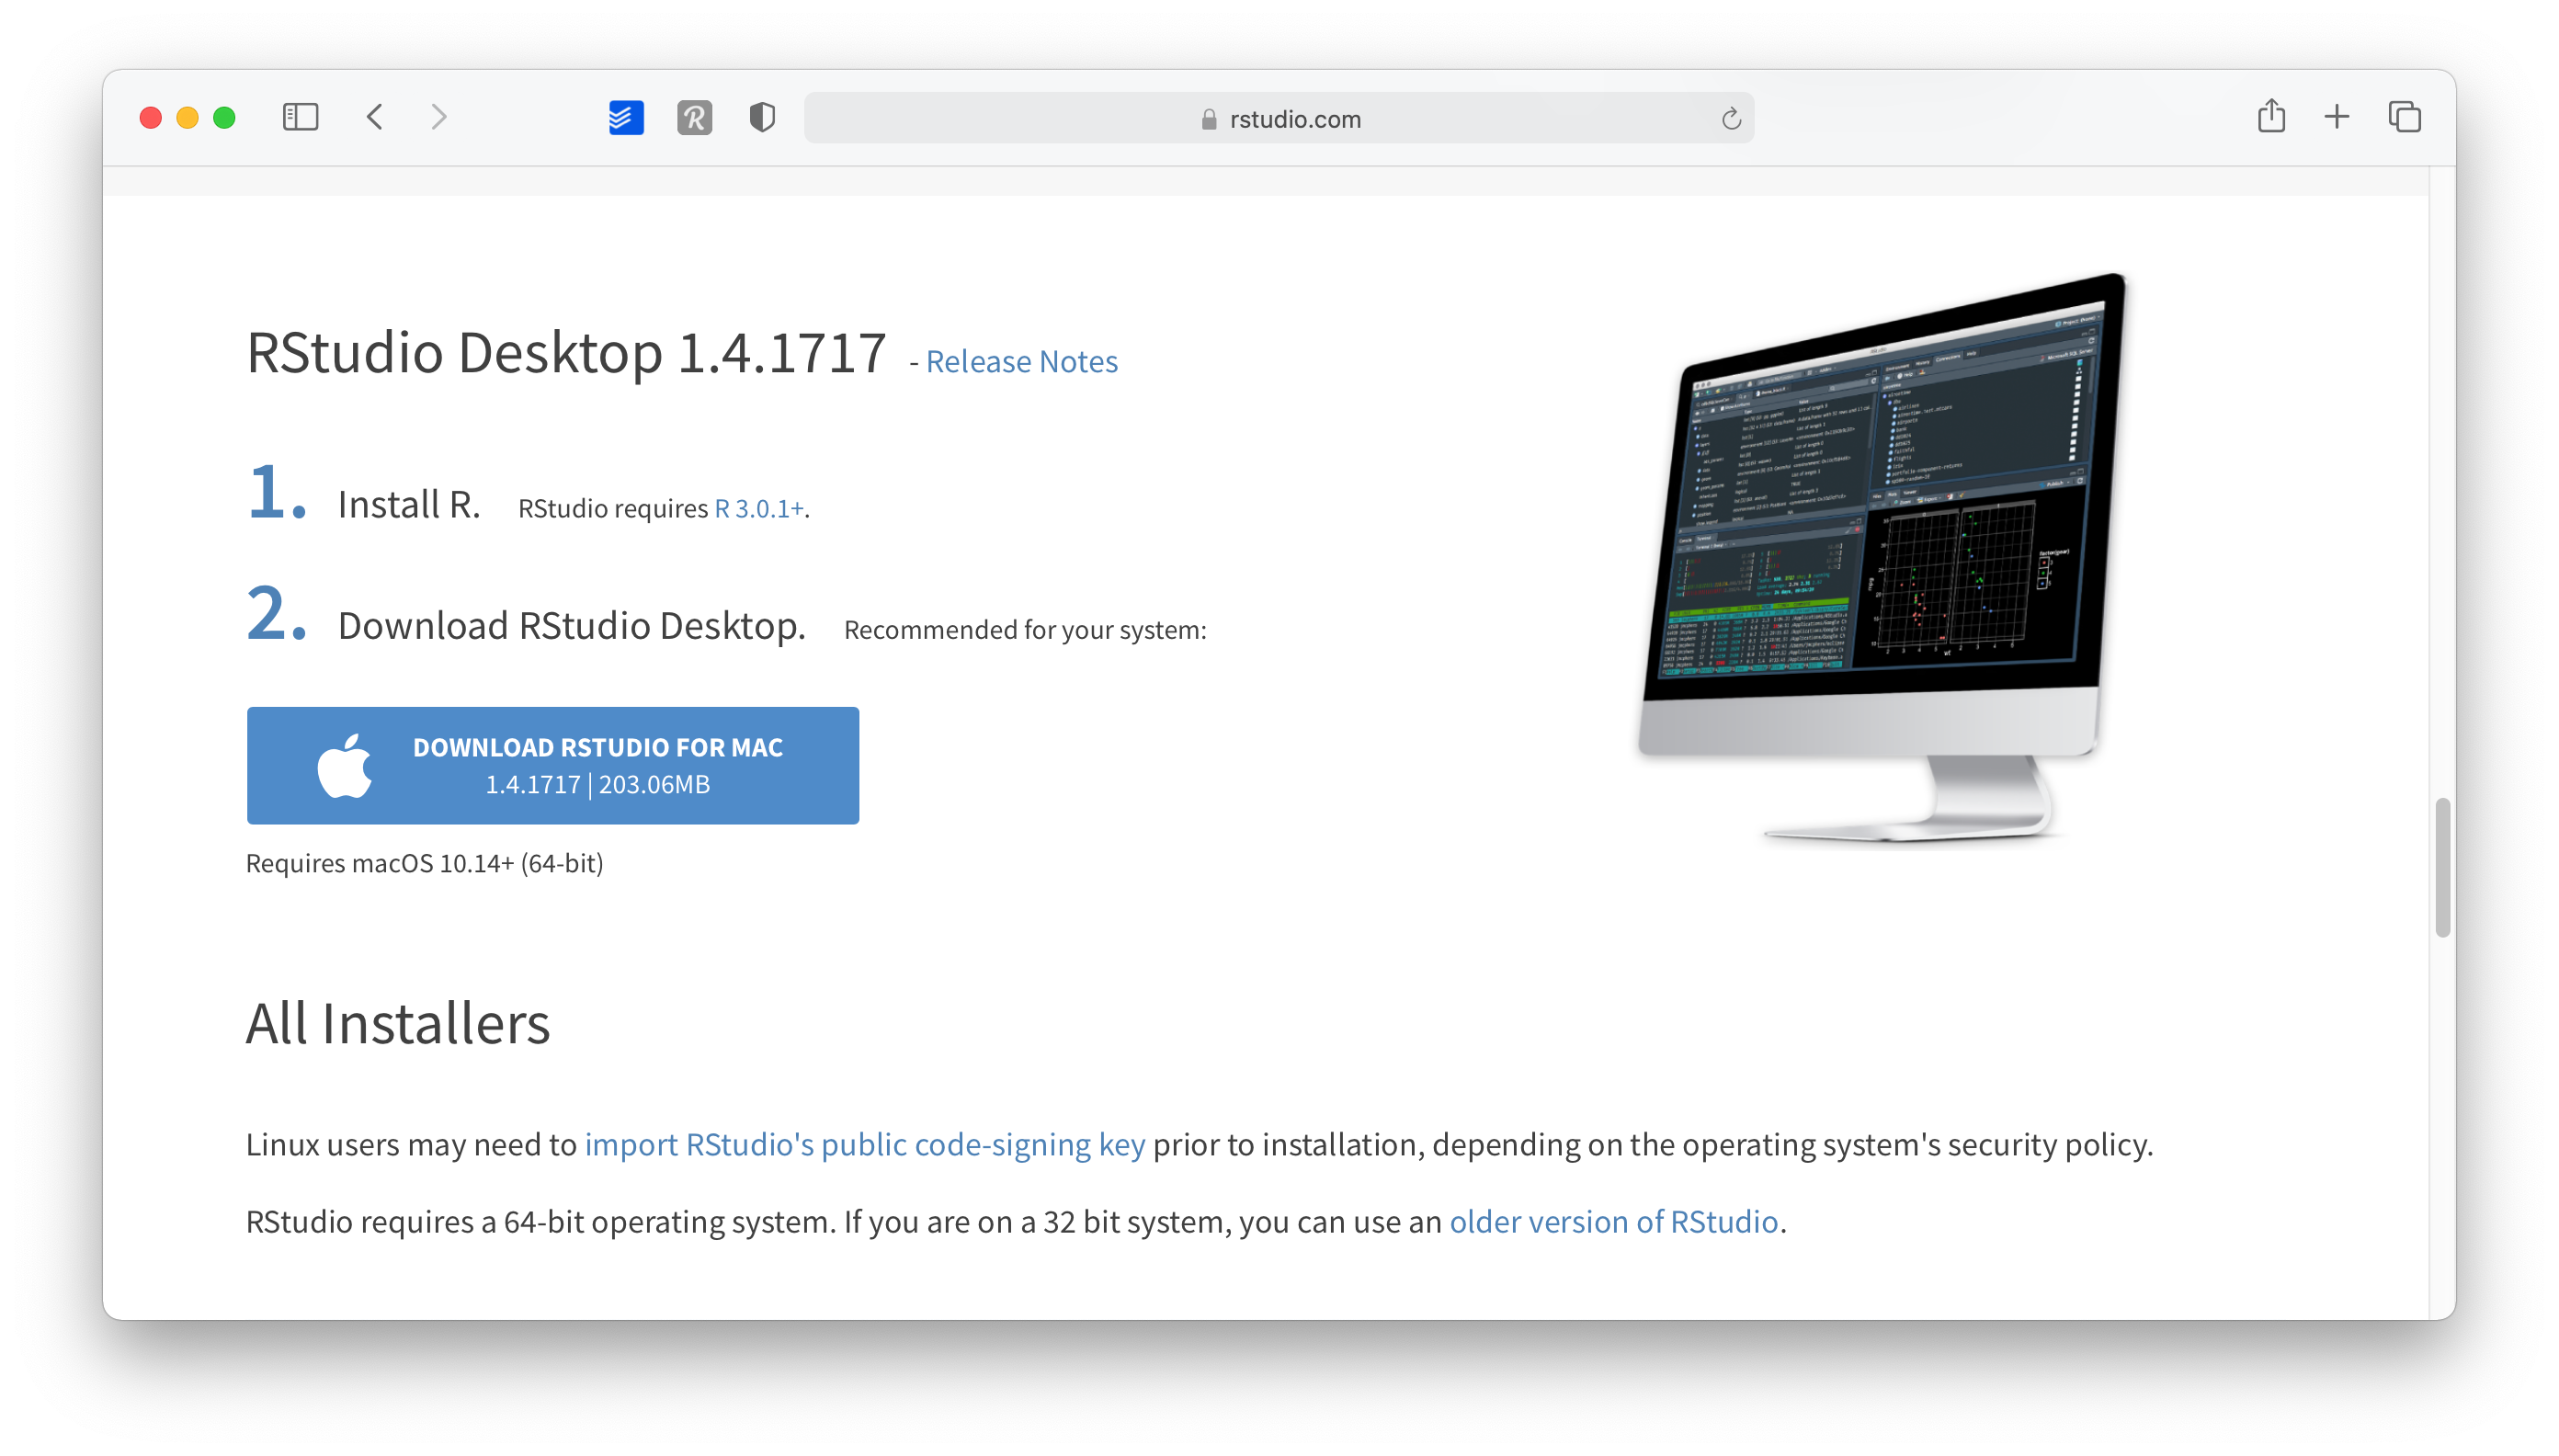
\includegraphics{images/chapter_03_img/rstudio/05_rstudio_download.png}
\item
  Open the downloaded file and follow the installation instructions (again, keep it to the default settings as much as possible)
\end{enumerate}

Congratulations, you are all set up to learn \emph{R}. From now on you only need to start RStudio and not \emph{R}. Of course, if you are the curious, nothing shall stop you to try \emph{R} without RStudio.

\hypertarget{when-you-first-start-rstudio}{%
\section{When you first start RStudio}\label{when-you-first-start-rstudio}}

Before you start programming away, you might want to make some tweaks to your settings right away to have a better experience (in my humble opinion). I recommend at least the following two changes by clicking on \texttt{RStudio\ \textgreater{}\ Preferences} or press \texttt{⌘/Ctrl\ +\ ,}.

\begin{enumerate}
\def\labelenumi{\arabic{enumi}.}
\item
  In the \texttt{Code\ \textgreater{}\ Editing} tab, make sure to have at least the first five options ticked, especially the \texttt{Auto-indent\ code\ after\ paste}. This setting will save time when trying to format your coding appropriately, making it easier to read. Indentation is the primary way of making your code look more readable and less like a series of characters that appear almost random.

  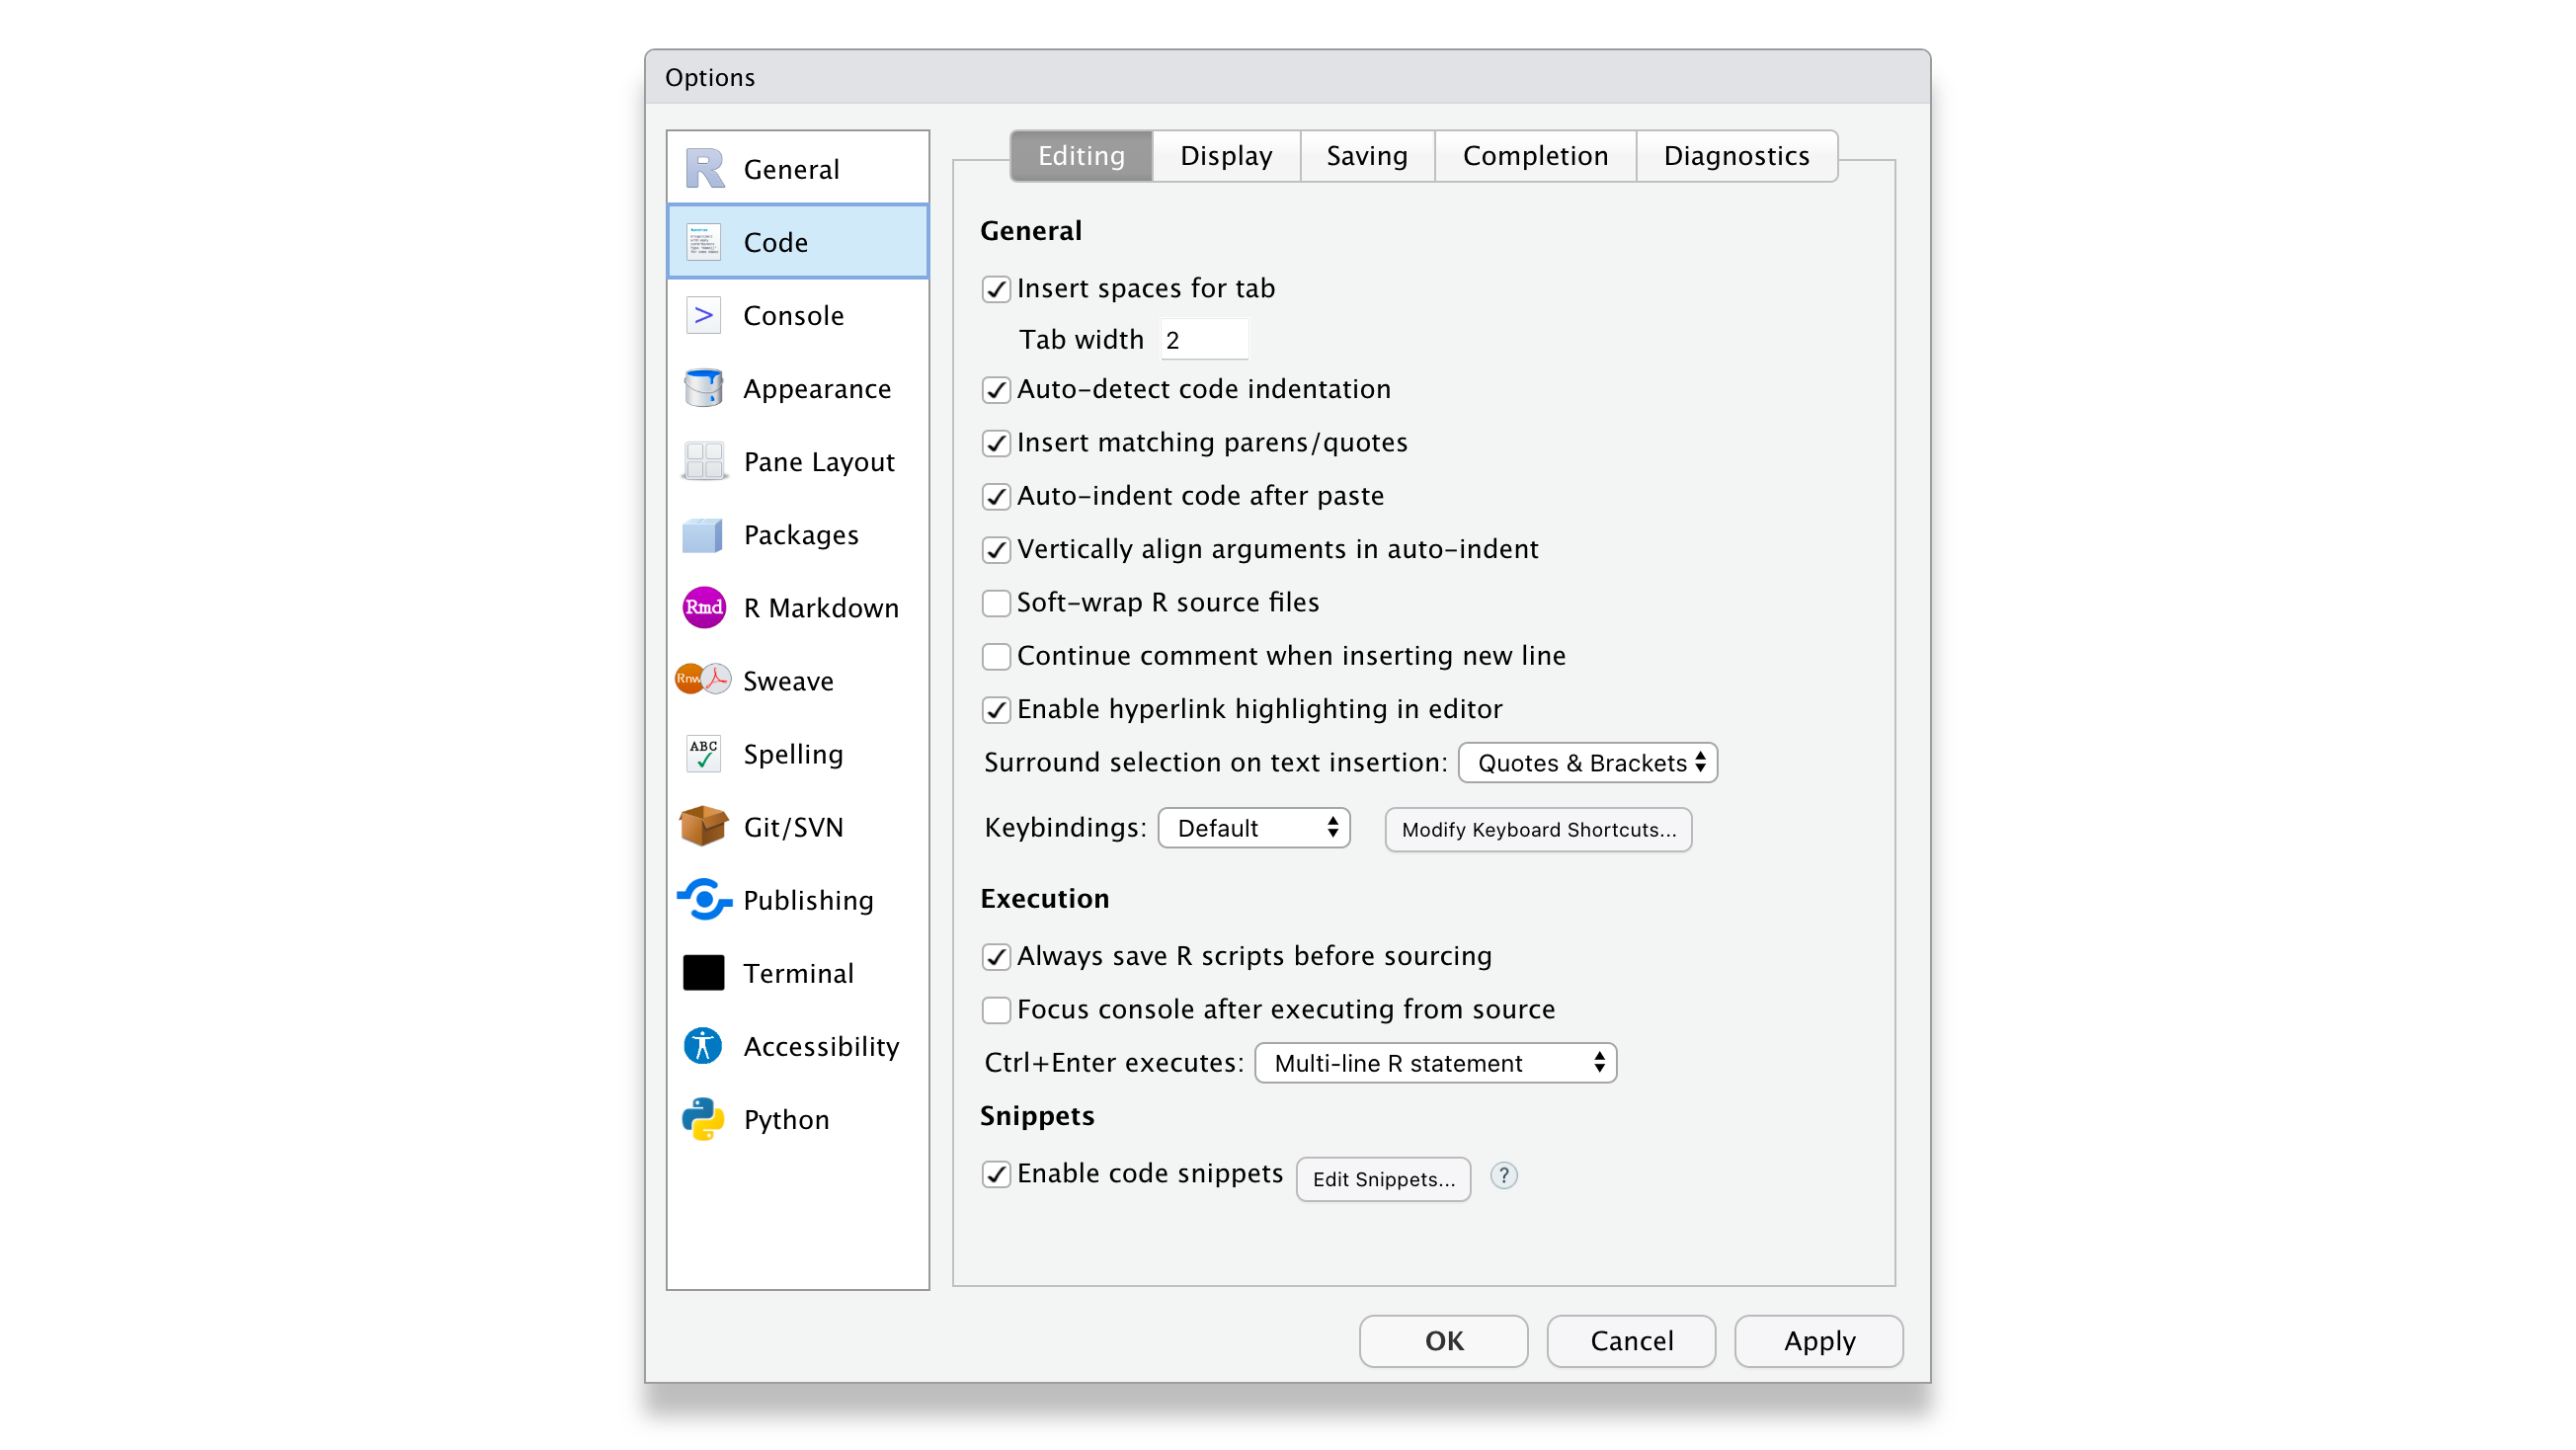
\includegraphics{images/chapter_03_img/rstudio_preferences/00_rstudio_preferences_editing.png}
\item
  In the \texttt{Display} tab, you might want to have the first three options selected. In particular, \texttt{Highlight\ selected\ line} is helpful because, in more complicated code, it is helpful to see where your cursor is.

  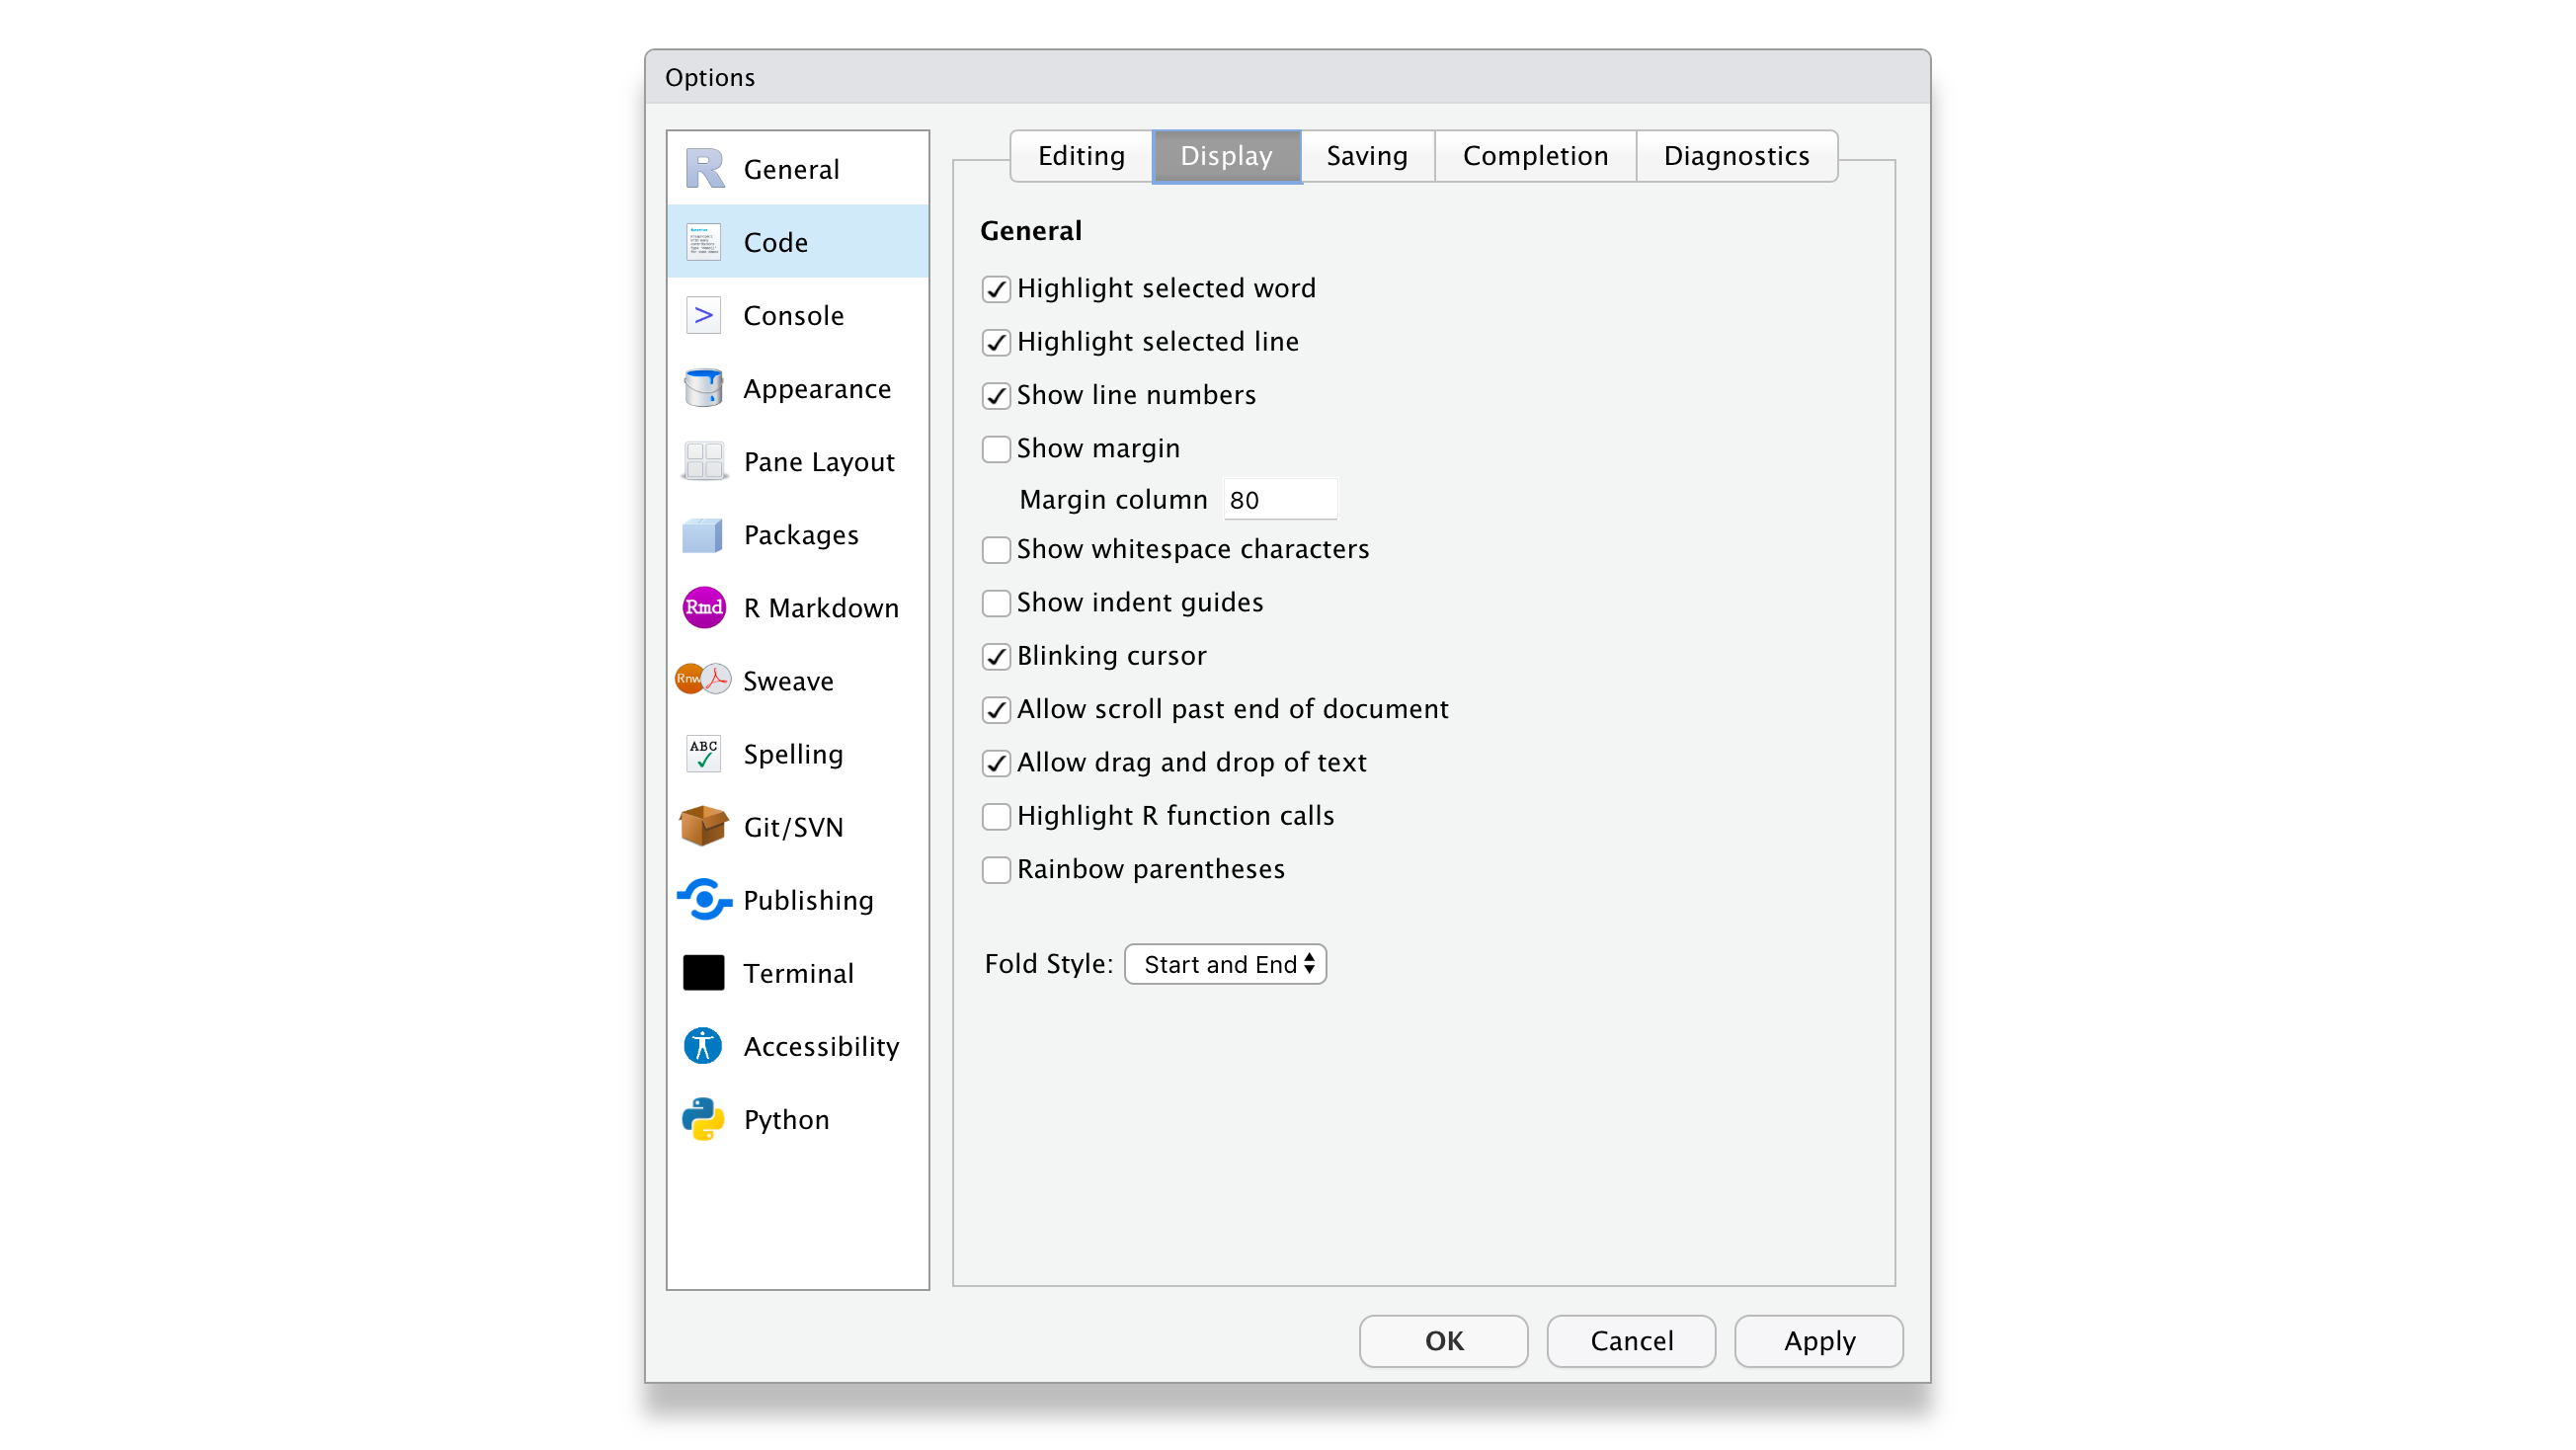
\includegraphics{images/chapter_03_img/rstudio_preferences/01_rstudio_preferences_display.png}
\end{enumerate}

Of course, if you wish to customise your workspace further, you can do so. The visually most impactful way to alter the default appearance of RStudio is to select Appearance and pick a completely different colour theme. Feel free to browse through various options and see what you prefer. There is no right or wrong here.

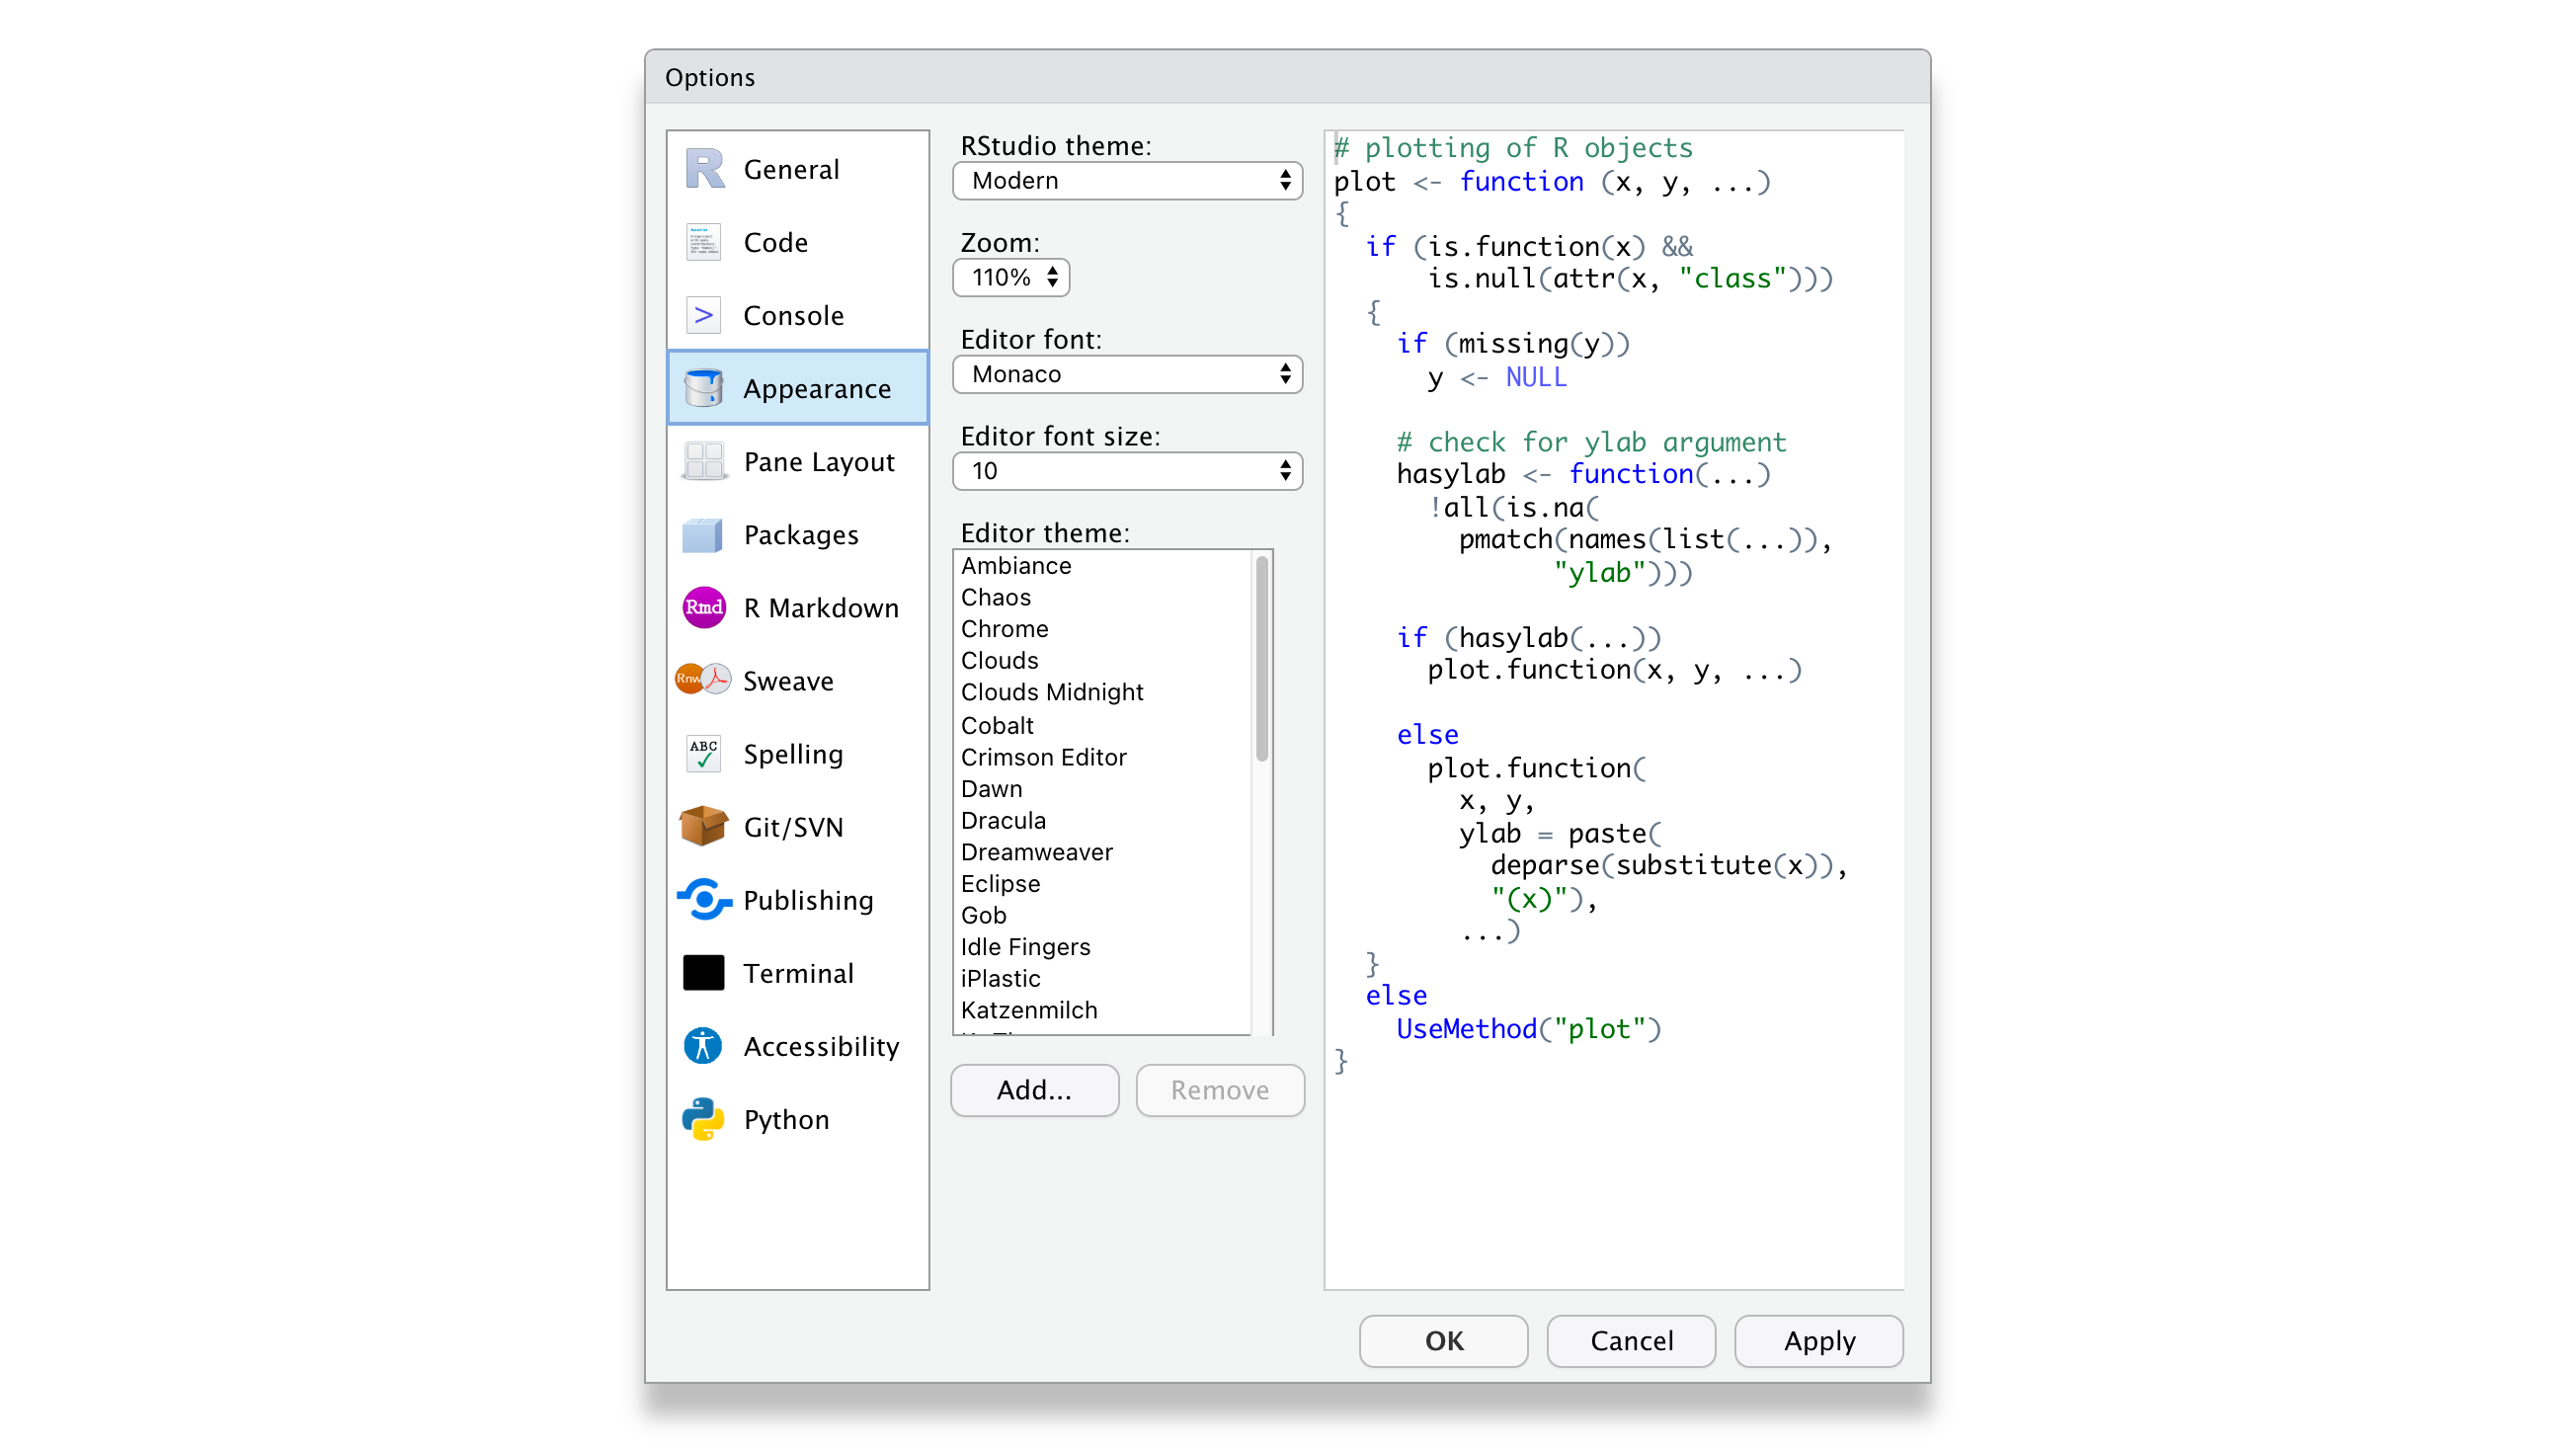
\includegraphics{images/chapter_03_img/rstudio_preferences/02_rstudio_preferences_appearance.png}

\hypertarget{updating-r-and-rstudio}{%
\section{Updating R and RStudio: Living at the pulse of innovation}\label{updating-r-and-rstudio}}

While not strictly something that helps you become a better programmer, this advice might come in handy to avoid turning into a frustrated programmer. When you update your software, you need to update R and RStudio separately from each other. While both R and RStudio work closely with each other, they still constitute separate pieces of software. Thus, it is essential to keep in mind that updating RStudio will not automatically update R. This can become problematic if specific packages you installed via RStudio (like a fancy learning algorithm) might not be compatible with earlier versions of R. Also, additional R packages developed by other people are separate pieces and are updated too, independently from R and RStudio.

I know what you are thinking: This already sounds complicated and cumbersome. However, rest assured, we take a look at how you can easily update all your packages with RStudio. Thus, all you need to remember is:~\emph{R}~needs to be updated separately from everything else.

\hypertarget{rstudio-cloud}{%
\section{RStudio Cloud}\label{rstudio-cloud}}

\texttt{to\ be\ completed}

\hypertarget{the-rstudio-interface}{%
\chapter{The RStudio Interface}\label{the-rstudio-interface}}

When you open RStudio for the first time, you are presented with four quadrants, each of which fulfils a unique purpose:

\begin{itemize}
\item
  The \texttt{Console} window,
\item
  The \texttt{Source} window,
\item
  The \texttt{Environment\ /\ History\ /\ Connections\ /\ Tutorial} window, and
\item
  The \texttt{Files\ /\ Plots\ /\ Packages\ /\ Help\ /\ Viewer} window
\end{itemize}

I will briefly explain the purpose of each window/pane and how they are relevant to your work in \emph{R}.

\hypertarget{the-console-window}{%
\section{The Console window}\label{the-console-window}}

The console is located in the bottom-left, and it is where you often will find the output of your coding and computations. It is also possible to write code directly into the console. Let's try the following example by calculating the sum of \texttt{10\ +\ 5}. Click into the console with your mouse, type the calculation into your console and hit \texttt{Enter/Return\ ↵} on your keyboard. The result should be pretty obvious:

\begin{Shaded}
\begin{Highlighting}[]
\CommentTok{\# We type the below into the console 👇}
\DecValTok{10}\SpecialCharTok{+}\DecValTok{5}
\DocumentationTok{\#\# [1] 15}
\end{Highlighting}
\end{Shaded}

Here is a screenshot of how it should look like at your end in RStudio:

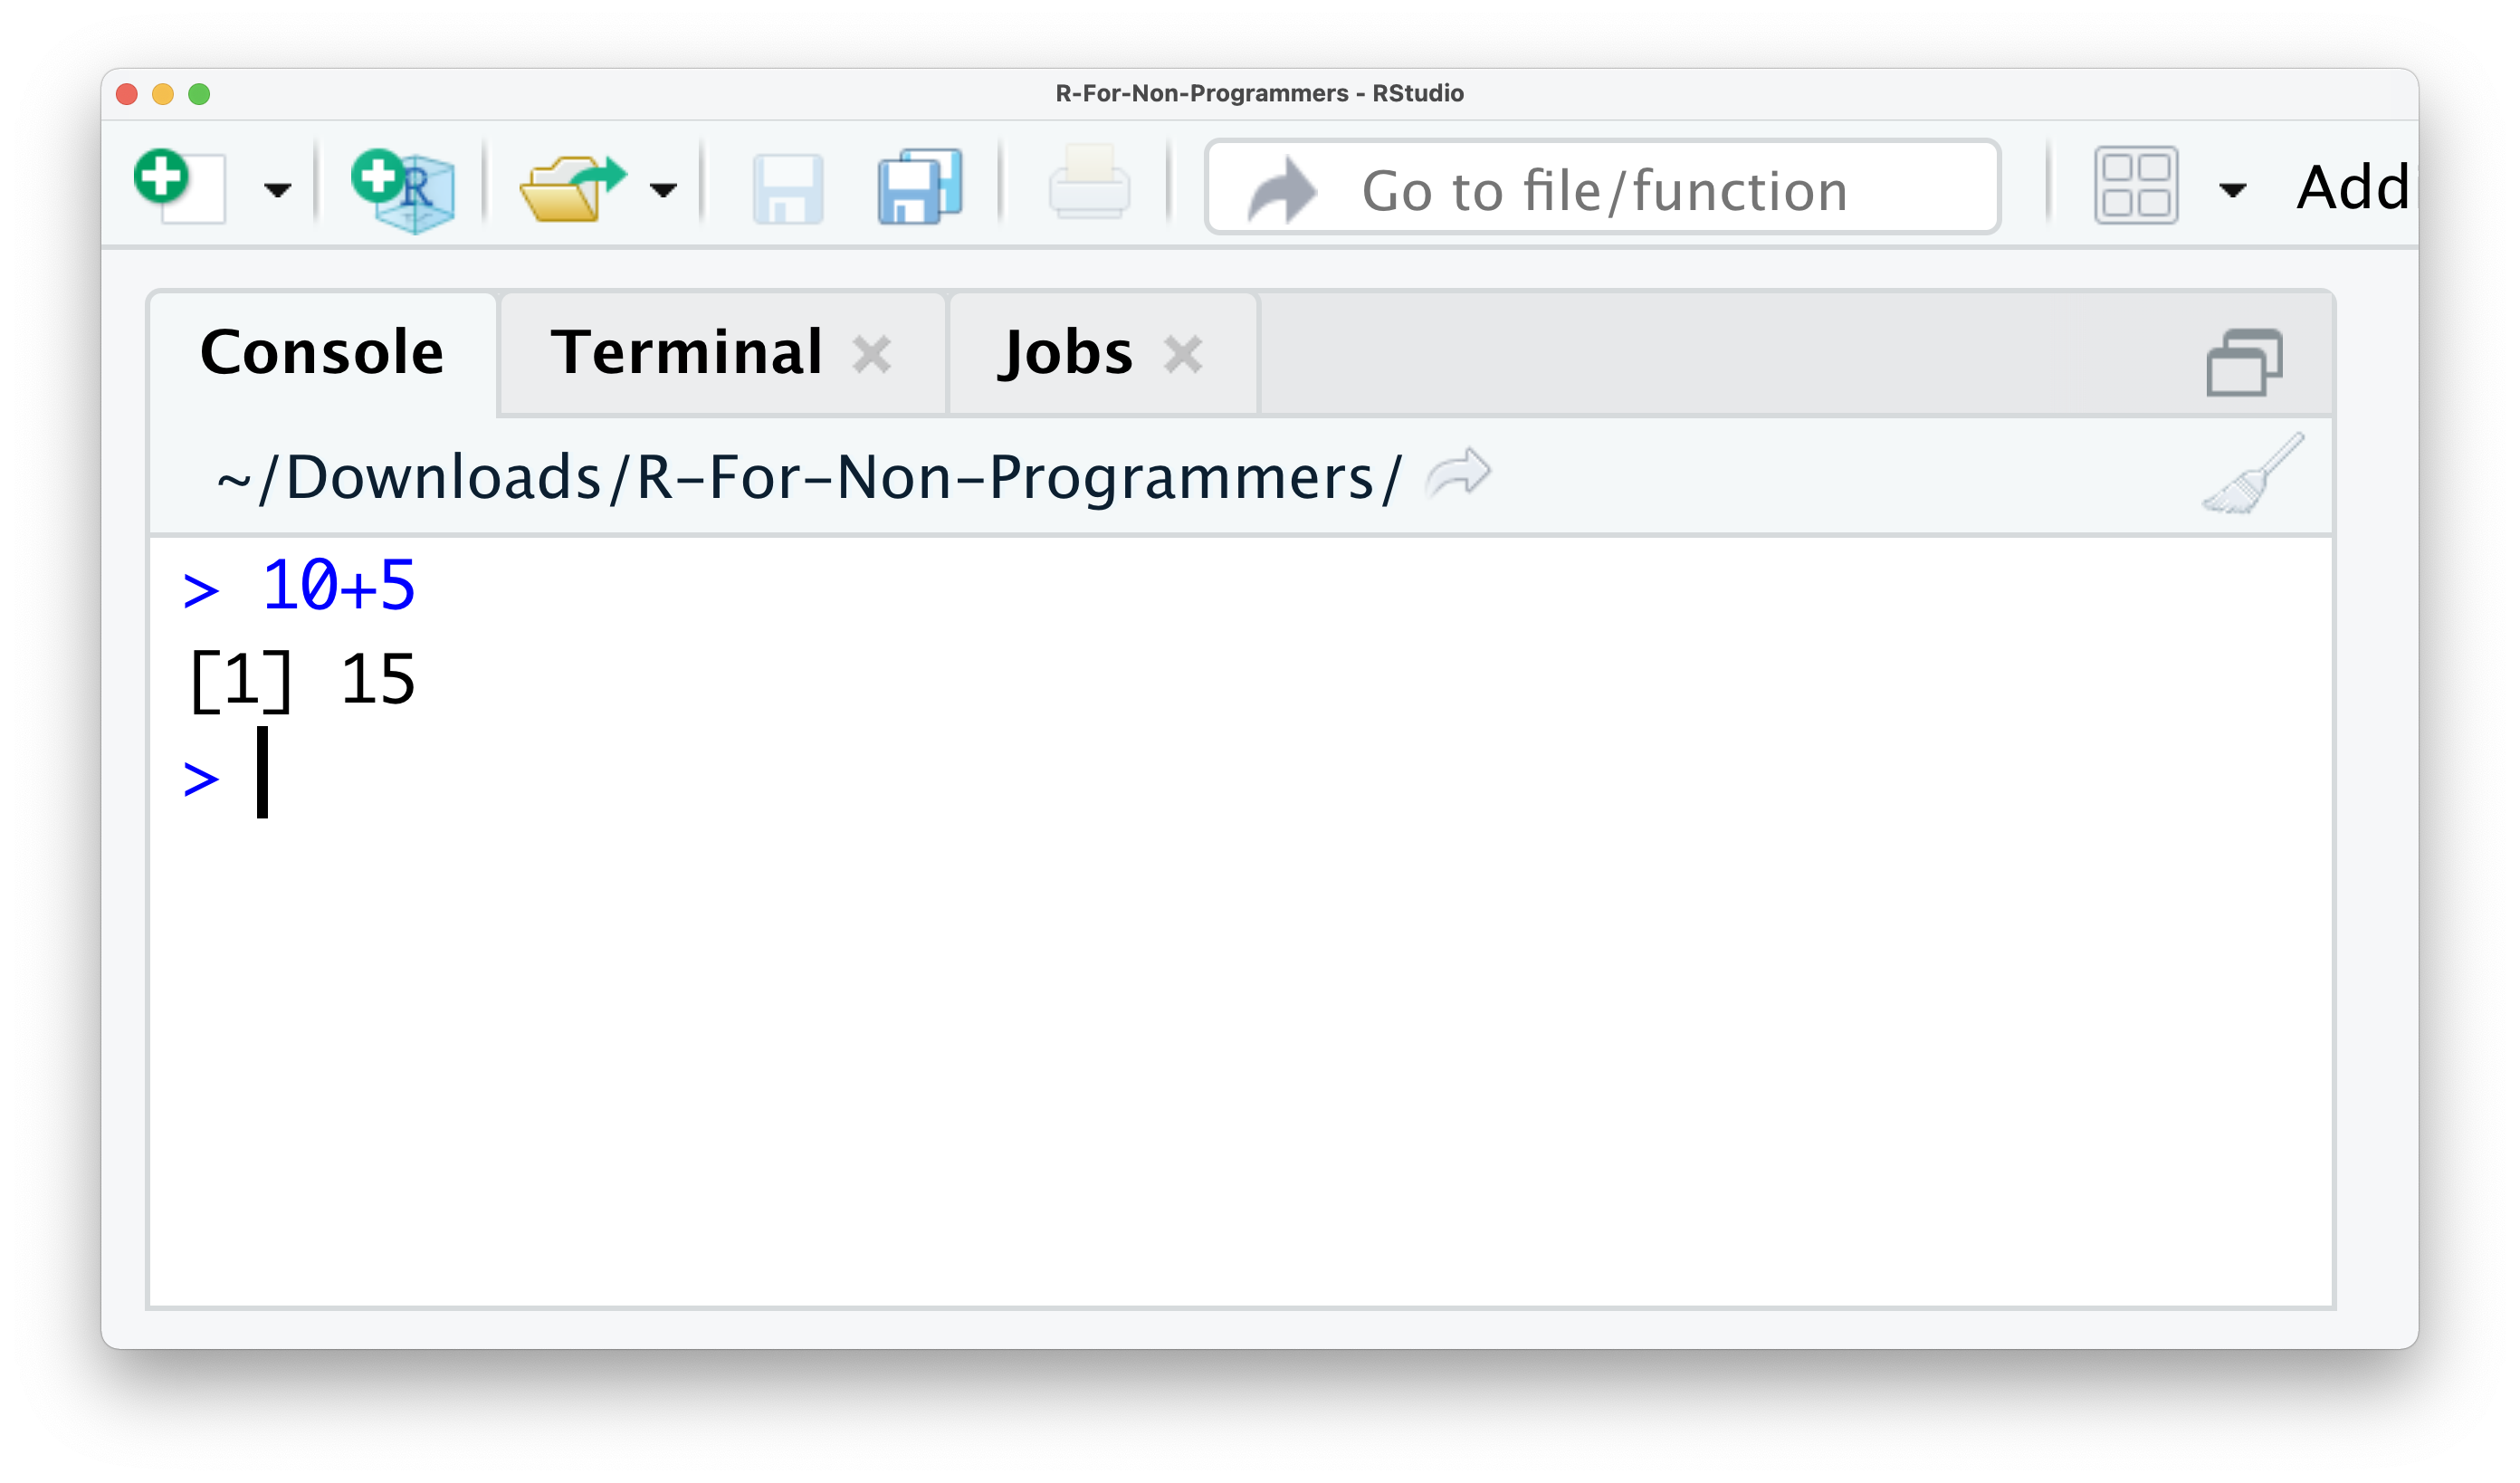
\includegraphics{images/chapter_04_img/02_console_window/console_algebra.png}

You just successfully performed your first successful computation. I know, this is not quite impressive just yet. \emph{R} is undoubtedly more than just a giant calculator.

In the top right of the console, you find a symbol that looks like a broom. This one is quite an important one because it clears your console. Sometimes the console can become very cluttered and difficult to read. If you want to remove whatever you computed, you can click the broom icon and clear the console of all text. I use it so frequently that I strongly recommend learning the keyboard shortcut, which is \texttt{Ctrl+L} on PC and Mac.

\hypertarget{the-source-window}{%
\section{The Source window}\label{the-source-window}}

In the top left, you can find the source window. The term `source' can be understood as any type of file, e.g.~data, programming code, notes, etc. The source panel can fulfil many functions, such as:

\begin{itemize}
\item
  Inspect data in an Excel-like format (LINK TO RELEVANT CHAPTER)
\item
  Open programming code, e.g.~an R Script (LINK TO RELEVANT CHAPTER)
\item
  Open other text-based file formats, e.g.

  \begin{itemize}
  \item
    Plain text (.txt),
  \item
    Markdown (.md),
  \item
    Websites (.html),
  \item
    LaTeX (.tex),
  \item
    BibTex (.bib),
  \end{itemize}
\item
  Edit scripts with code in it,
\item
  Run the analysis you have written.
\end{itemize}

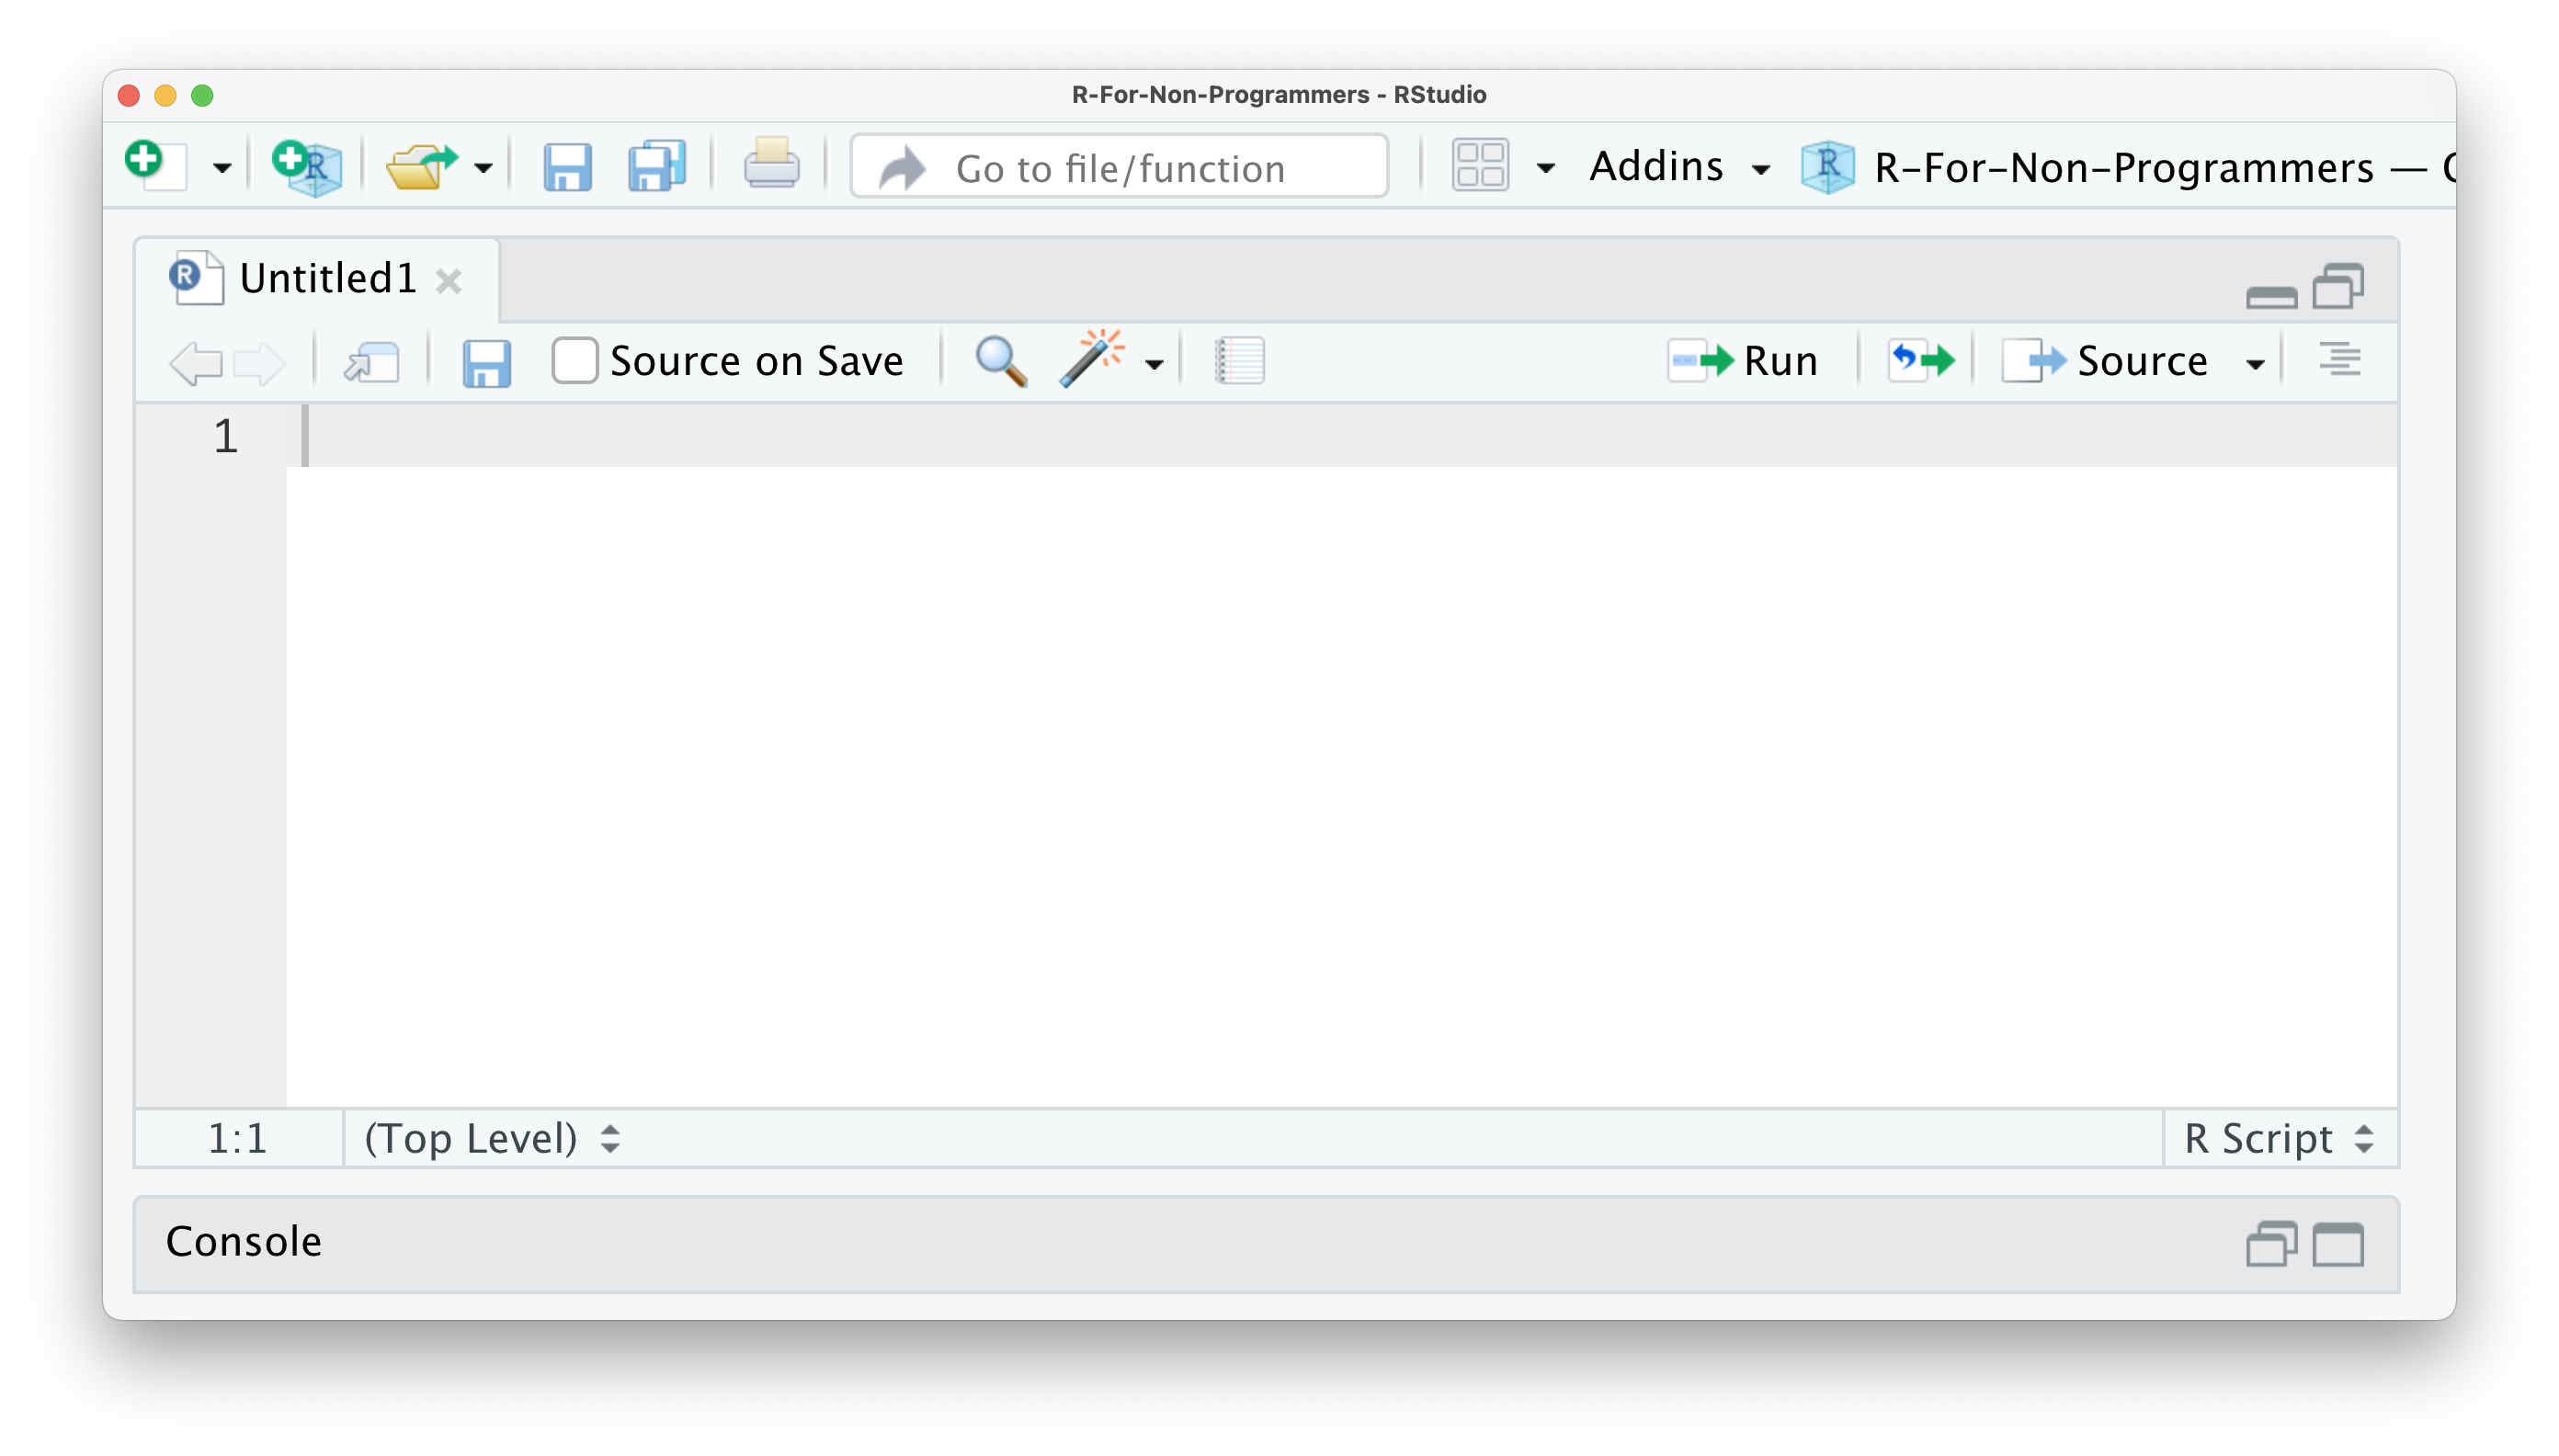
\includegraphics{images/chapter_04_img/03_source_window/01_rstudio_source.png}

In other words, the source window will show you whatever file you are interested in, as long as RStudio can read it - and no, Microsoft Office Documents are not supported. Another limitation of the source window is that it can only show text-based files. So opening images, etc. would not work.

\hypertarget{the-environment-history-connections-tutorial-window}{%
\section{The Environment / History / Connections / Tutorial window}\label{the-environment-history-connections-tutorial-window}}

The window in the top right shows multiples panes. The first pane is called \emph{Environment} and shows you objects which are available for computation. One of the first objects you will create is your dataset because, without data, we cannot perform any analysis. Thus, one object might be your data. Another object could be a plot showing the number of male and female participants in your study. To find out how to create objects yourself, you can take a glimpse at (INSERT CHAPTER X). Besides datasets and plots, you will also find other objects here, e.g.~lists, vectors and functions you created yourself. Don't worry if none of these words makes sense at this point. We will cover each of them in the upcoming chapters. For now, remember this is a place where you can find different objects you created.

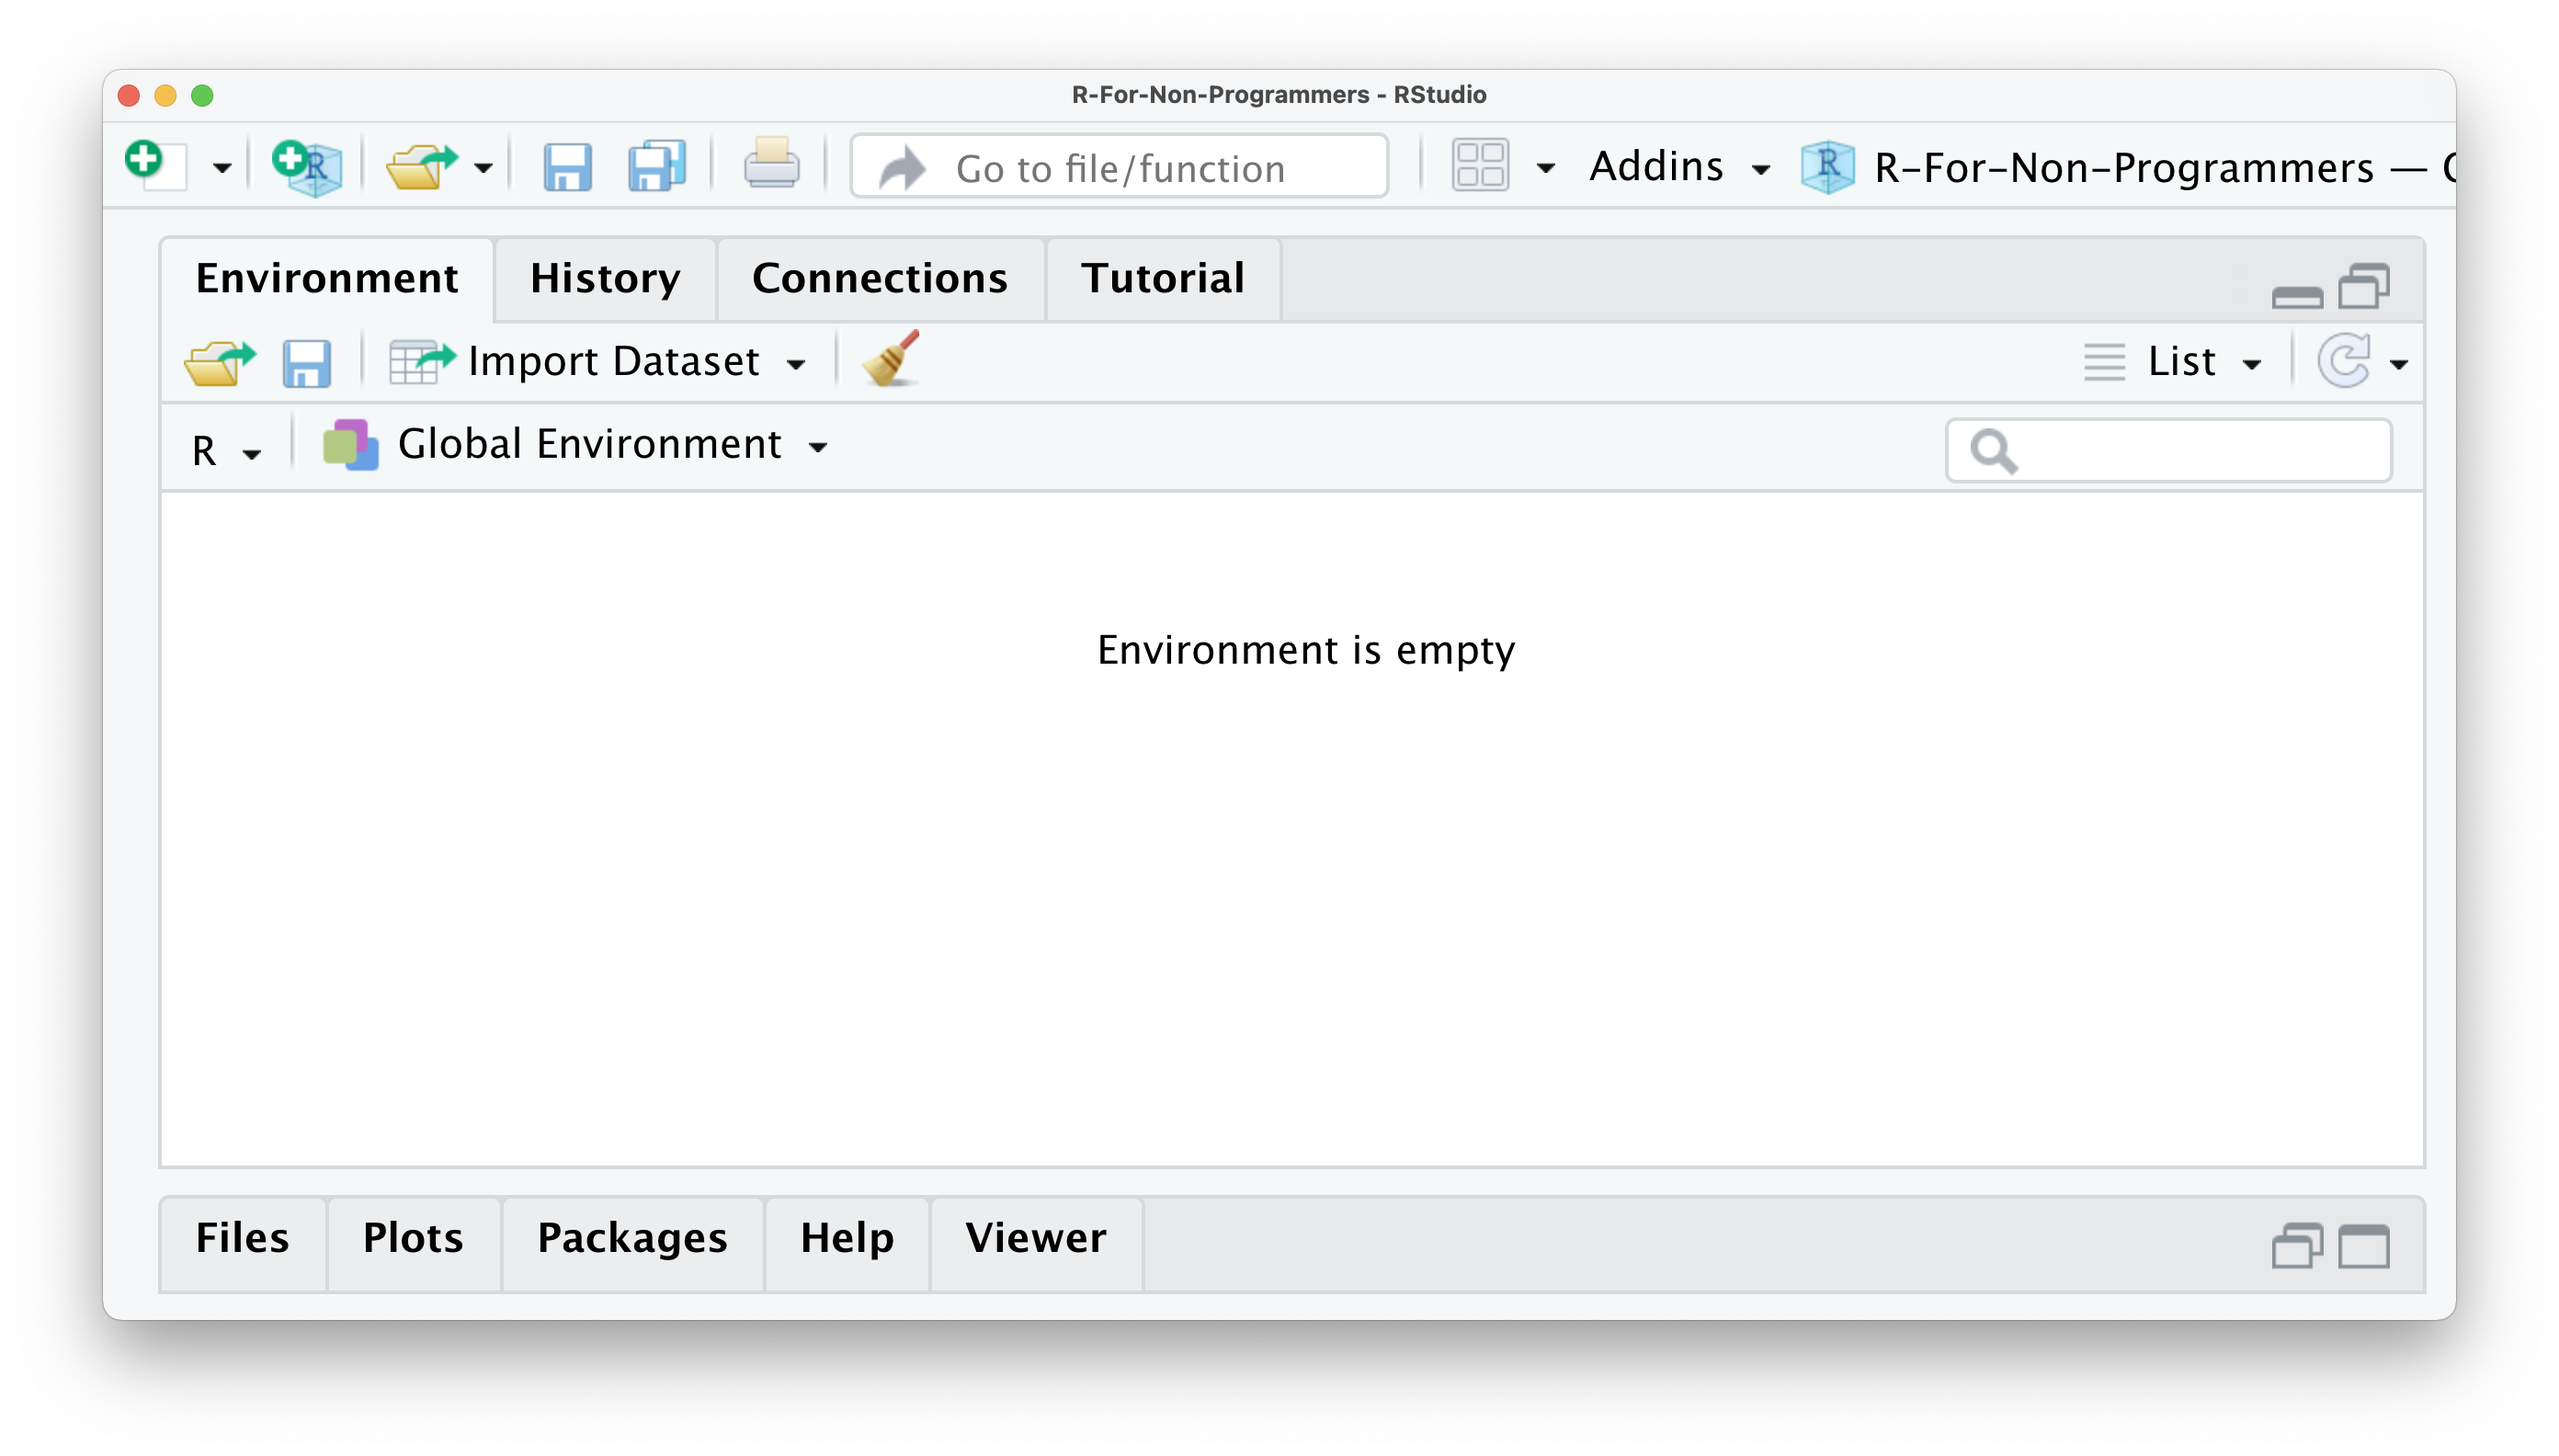
\includegraphics{images/chapter_04_img/04_environment_history_etc/01_rstudio_environment.png}

The \emph{History} pane is very easy to understand. Whatever computation you run in the Console will be stored. So you can go back and see what you coded and rerun that code. Remember the example from above where we computed the sum of \texttt{10+5}? This computation is stored in the history of RStudio, and you can rerun it by clicking on \texttt{10+5} in the history pane and then click on \texttt{To\ Console}. This will insert \texttt{10+5} back into the Console, and we can hit \texttt{Return\ ↵} to retrieve the result. You also have the option to copy the code into an existing or new R Script by clicking on \texttt{To\ Source}. By doing this, you can save this computation on your computer and reuse it later. Finally, if you would like to store your history, you can do so by clicking on the \texttt{floppy\ disk\ symbol}. There are two more buttons in this pane, one allows you to delete individual entries in the history, and the last one, a \texttt{broom}, clears the entire history (irrevocably).

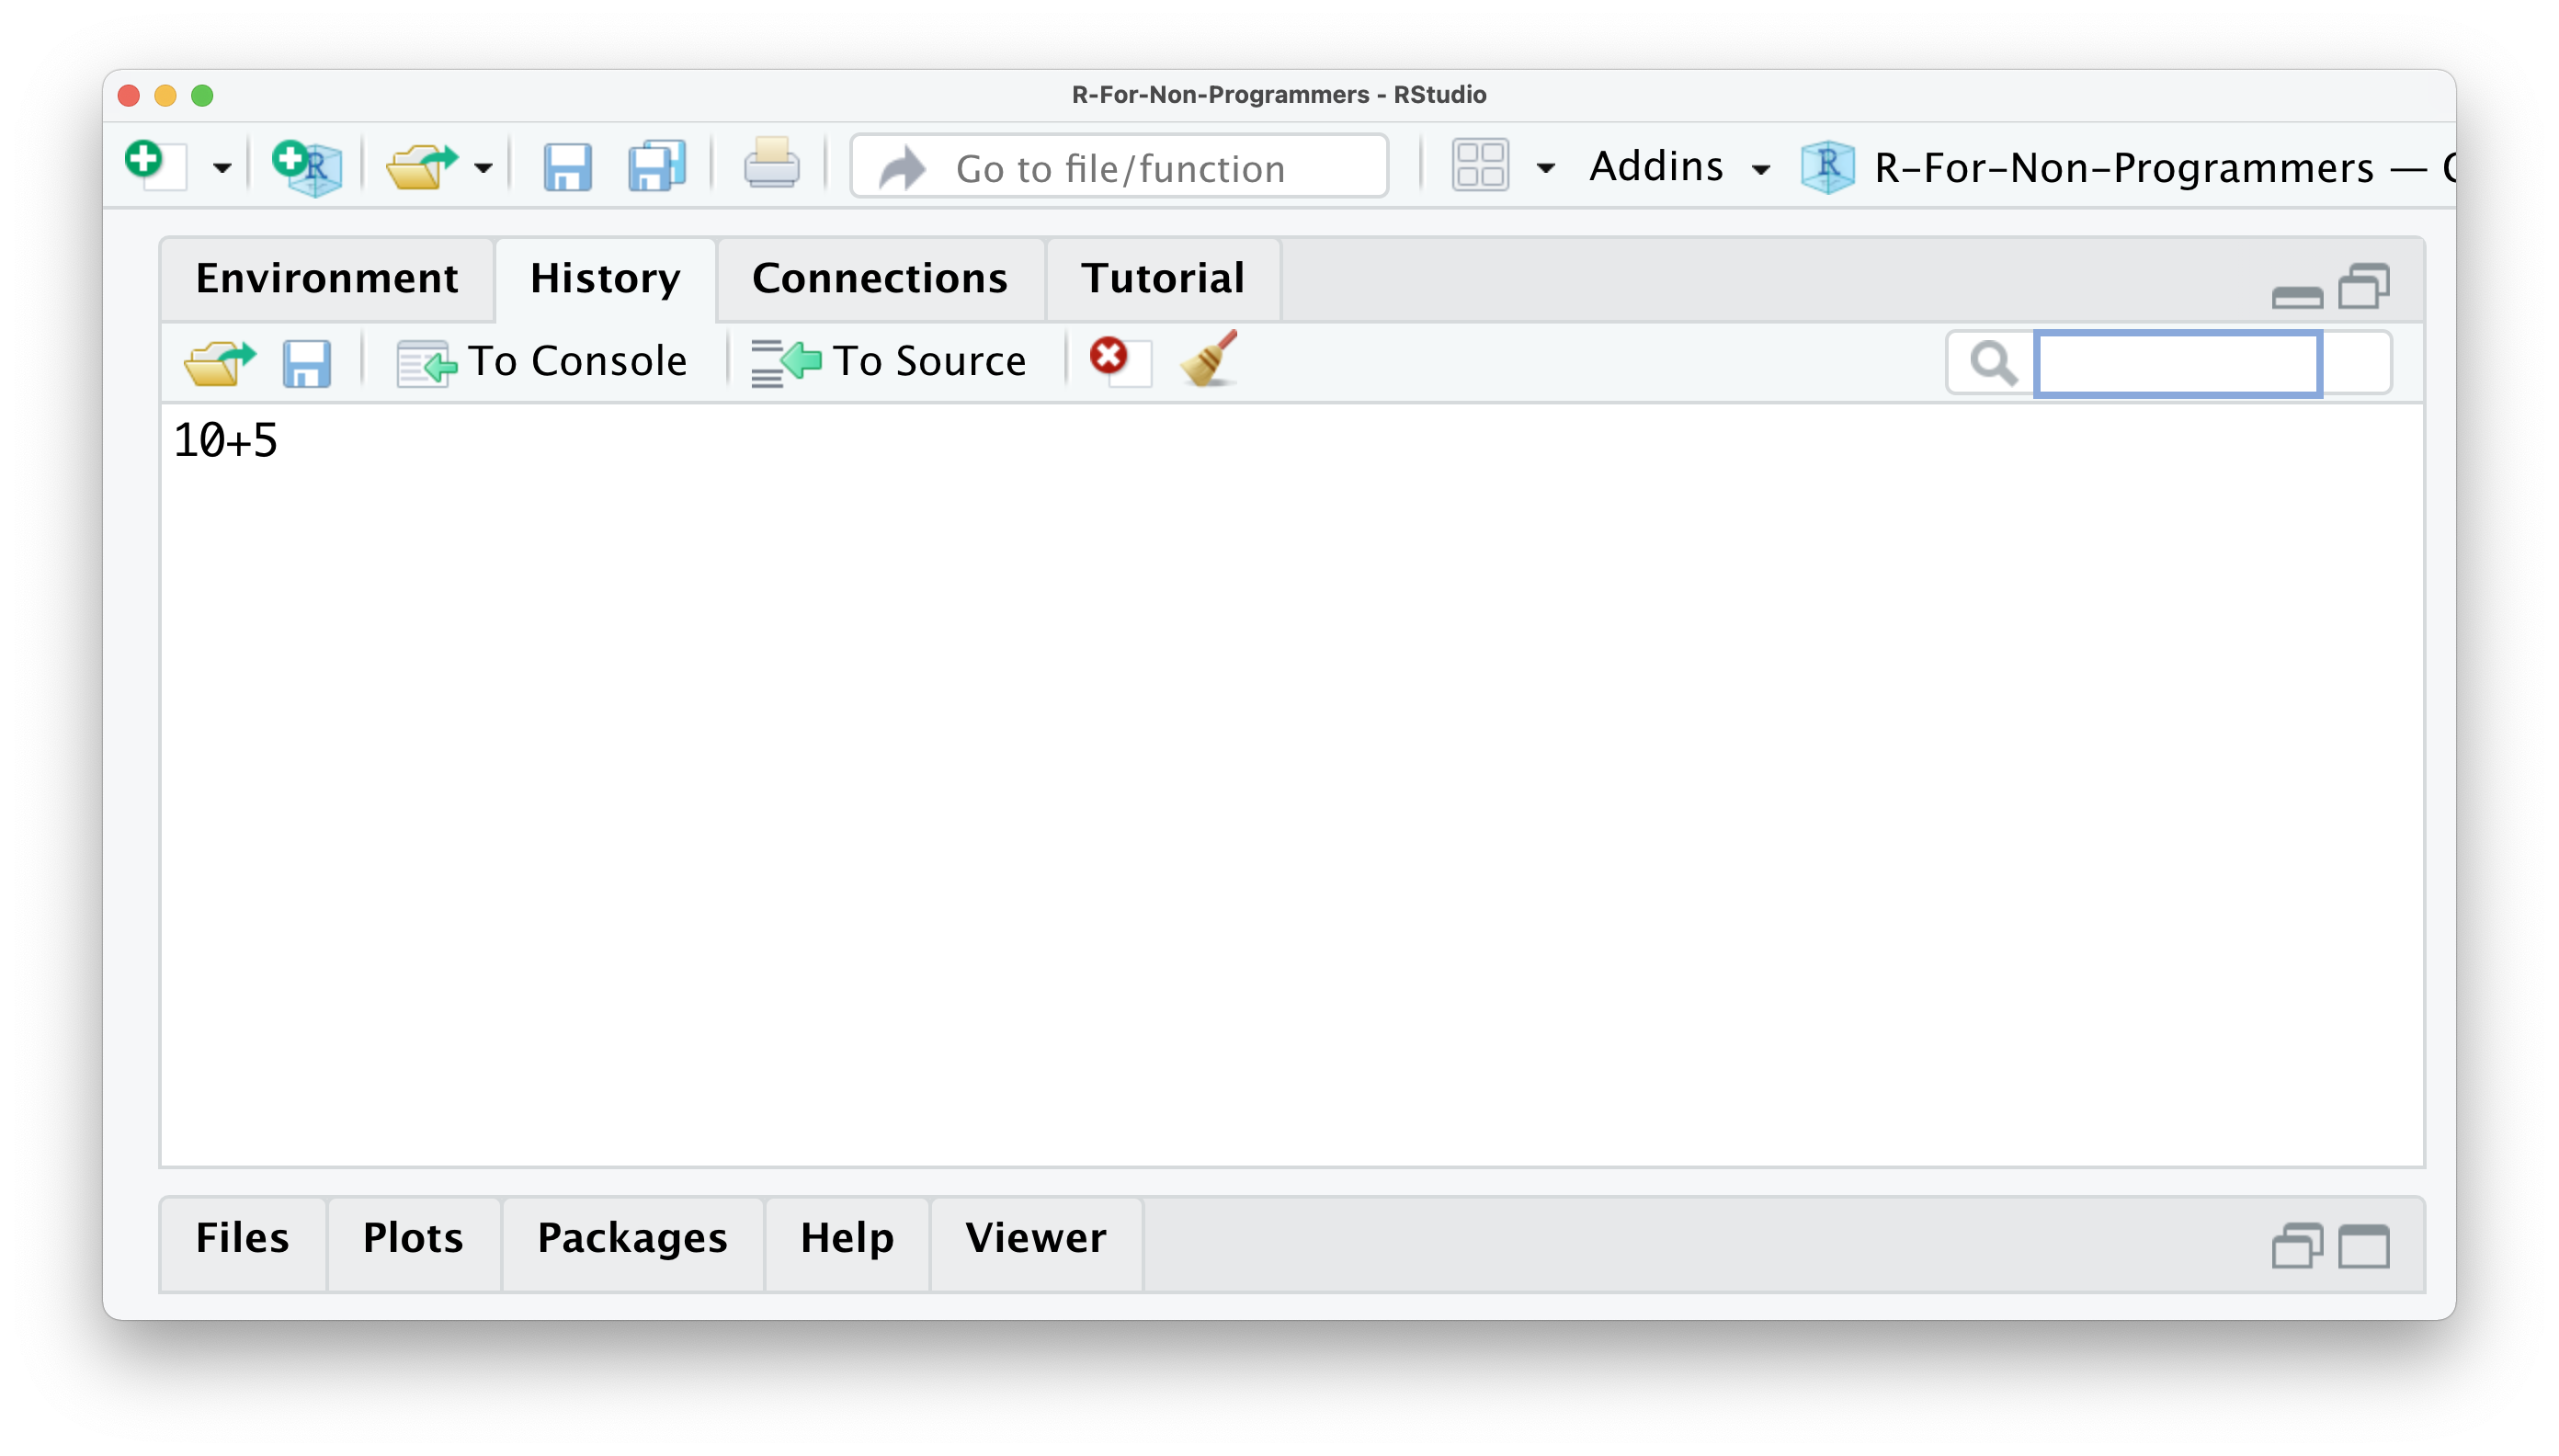
\includegraphics{images/chapter_04_img/04_environment_history_etc/02_rstudio_history.png}

The pane \emph{Connections} allows you to tab into external databases directly. This can come in handy when you work collaboratively on the same data or want to work with extensive datasets without having to download them. However, for an introduction to R, we will not use this feature of RStudio for now.

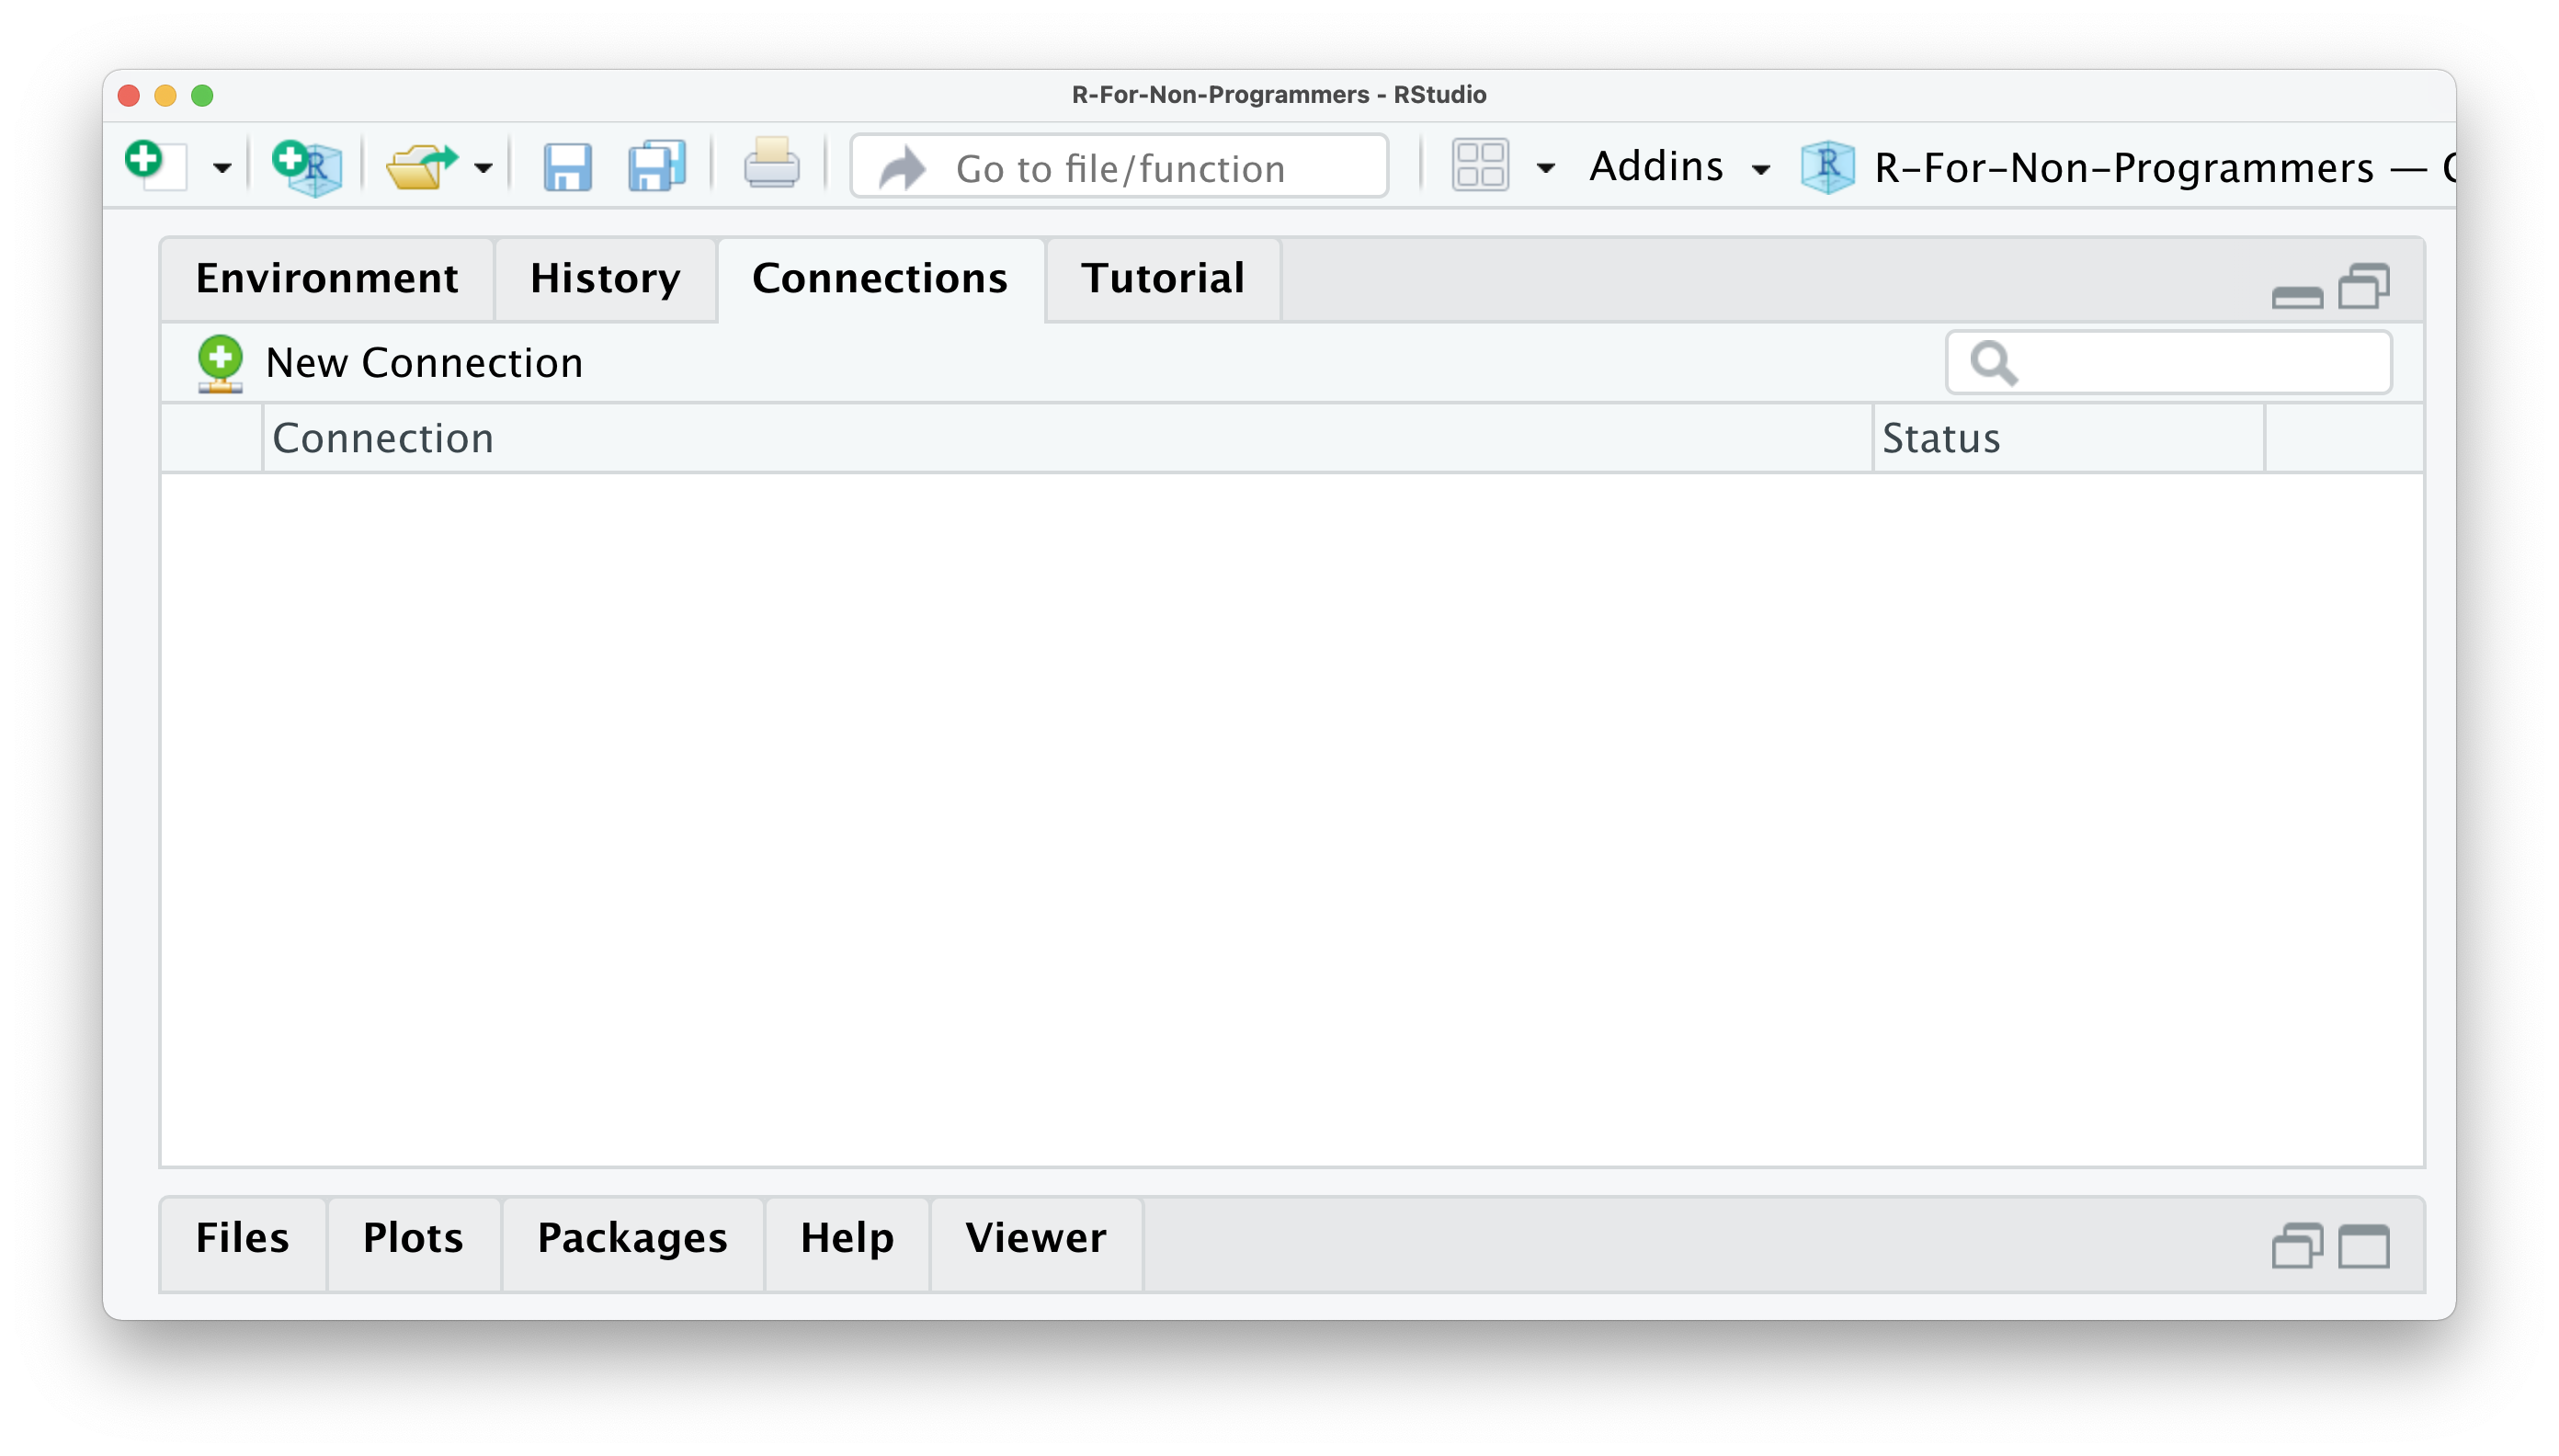
\includegraphics{images/chapter_04_img/04_environment_history_etc/03_rstudio_connections.png}

The last pane is called \emph{Tutorial}. Here you can find additional materials to learn \emph{R} and RStudio. If you search for more great content to learn R, this serves as a great starting point.

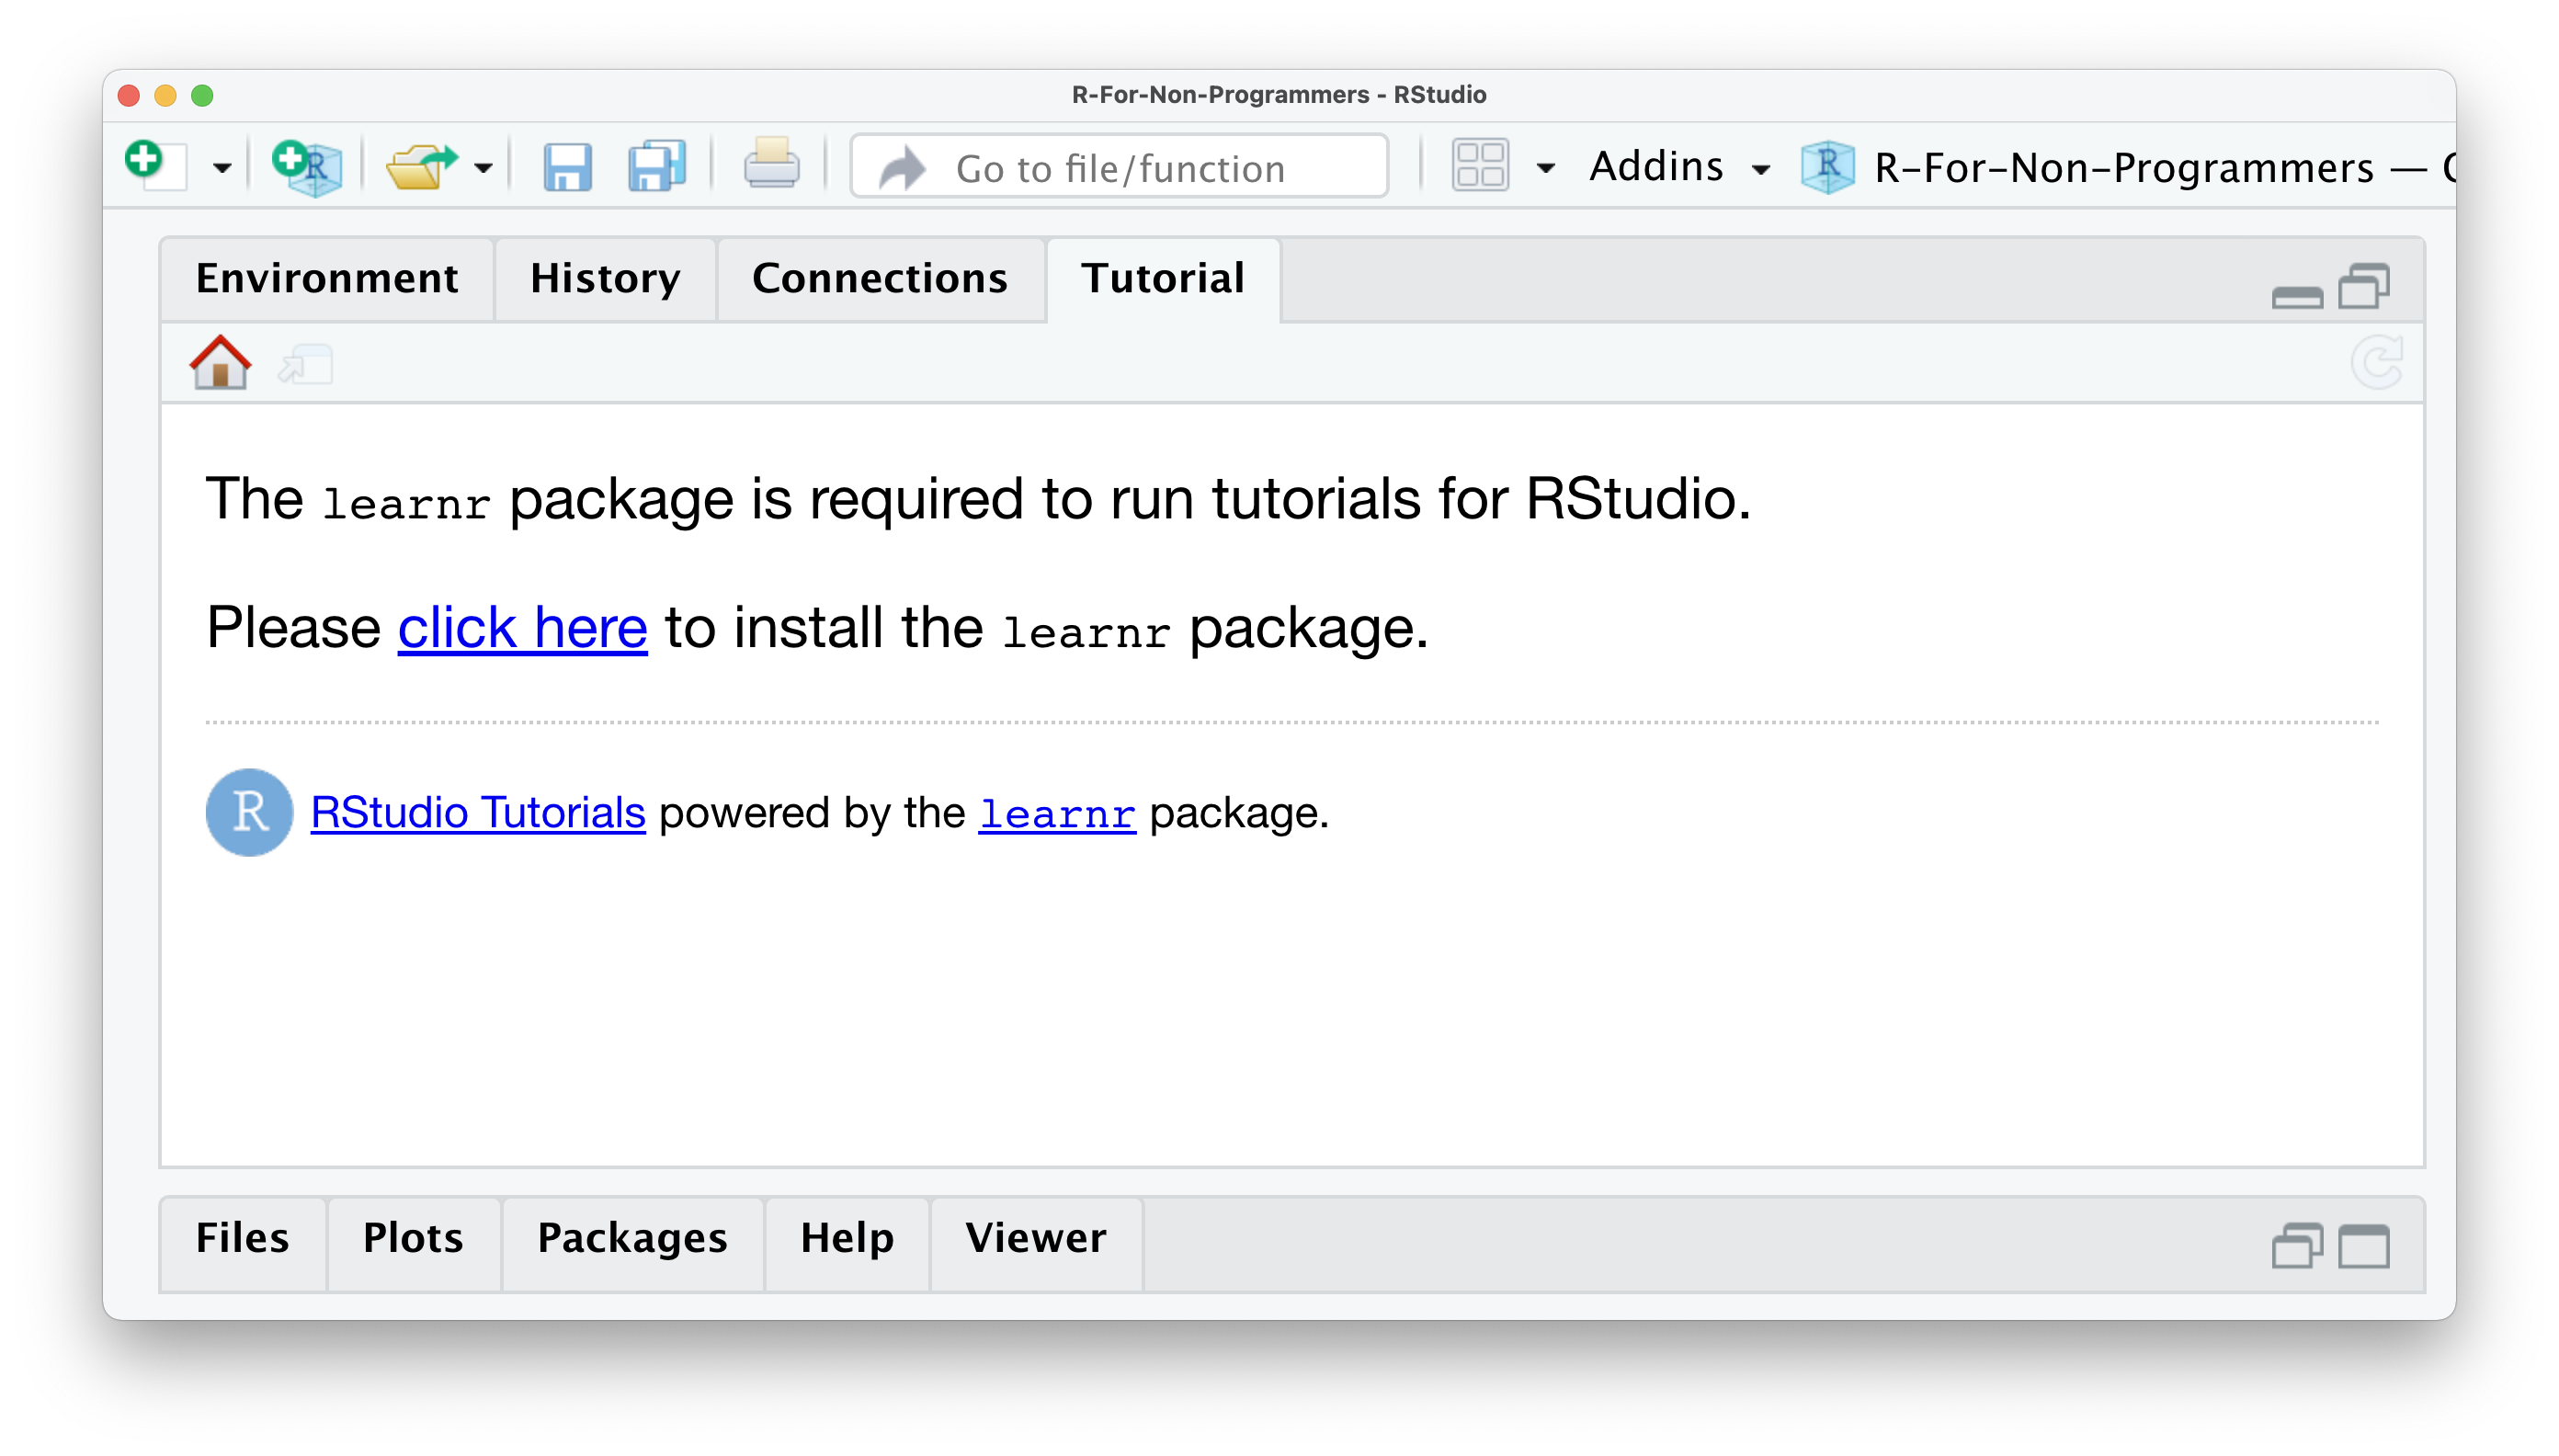
\includegraphics{images/chapter_04_img/04_environment_history_etc/04_rstudio_tutorial.png}

\hypertarget{the-files-plots-packages-help-viewer-window}{%
\section{The Files / Plots / Packages / Help / Viewer window}\label{the-files-plots-packages-help-viewer-window}}

The last window consists of five essential panes. The first one is the \emph{Files} pane. As the name indicates, it lists all the files and folders in your root directory. A root directory is the default directory where RStudio saves your files, for example, your analysis. However, you can easily change this directory to something else (see also CHAPTER X) or use R Project files (see CHAPTER X) to carry out your research. Thus, the \emph{Files} pane is an easy way to load data into RStudio and create folders to keep your research project well organised.

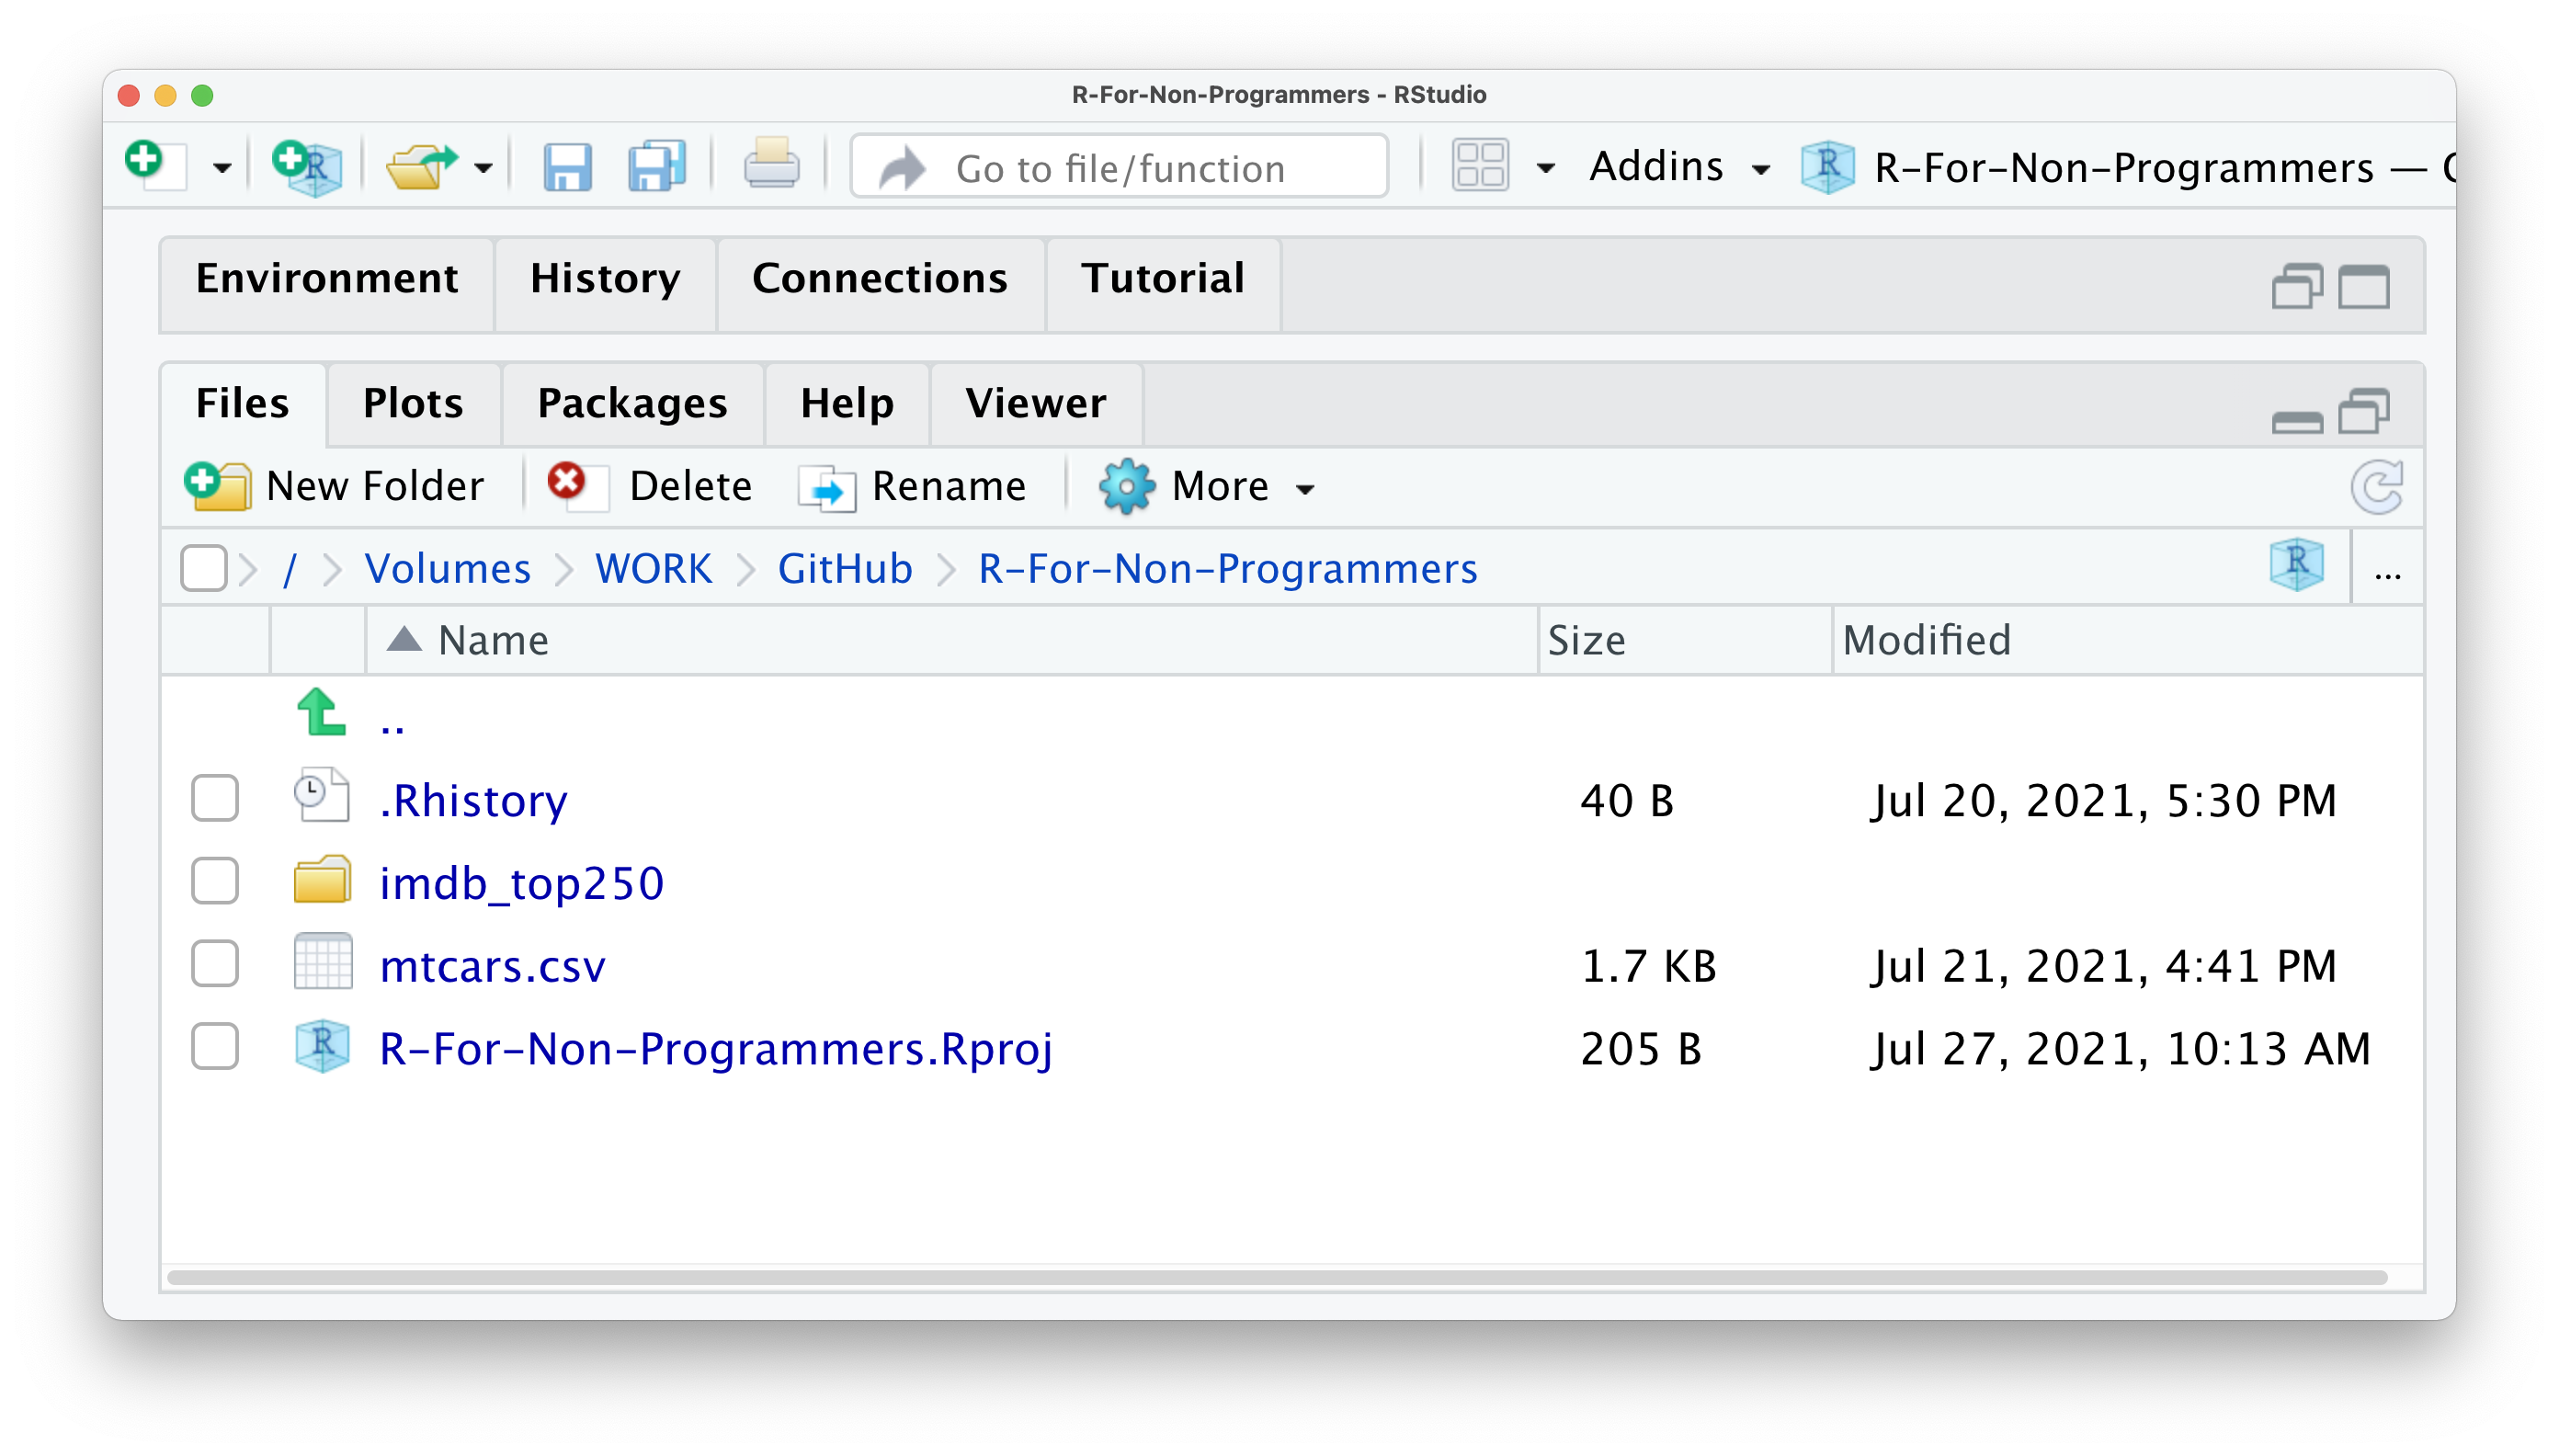
\includegraphics{images/chapter_04_img/05_files_plots_etc/01_rstudio_files.png}

Since the Console cannot reproduce data visualisations, RStudio offers a way to do this very easily. It is through the Plots pane. This pane is exclusively designed to show you any plots you have created using R. Here is a simple example that you can try. Type into your console \texttt{boxplot(mtcars\$hp)}.

\begin{Shaded}
\begin{Highlighting}[]
\CommentTok{\# Here we create a nice boxplot using a dataset called \textquotesingle{}mtcars\textquotesingle{}}
\FunctionTok{boxplot}\NormalTok{(mtcars}\SpecialCharTok{$}\NormalTok{hp)}
\end{Highlighting}
\end{Shaded}

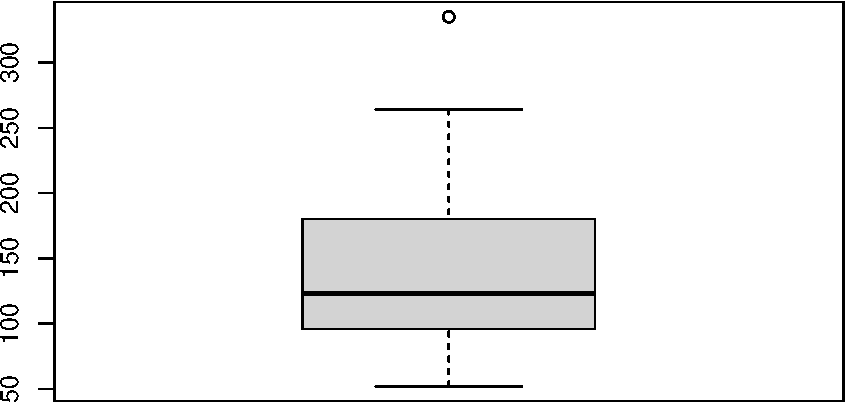
\includegraphics{r_for_non_programmers_files/figure-latex/Simple boxplot-1.pdf}

Although this is a short piece of coding, it performs quite a lot of steps:

\begin{itemize}
\item
  it uses a function called \texttt{boxplot()} to draw a boxplot of
\item
  a variable called \texttt{hp} (for horsepower), which is located in
\item
  a dataset named \texttt{mtcars},
\item
  and it renders the graph in your \emph{Plots} pane
\end{itemize}

This is how the plot should look like in your RStudio \emph{Plots} pane.

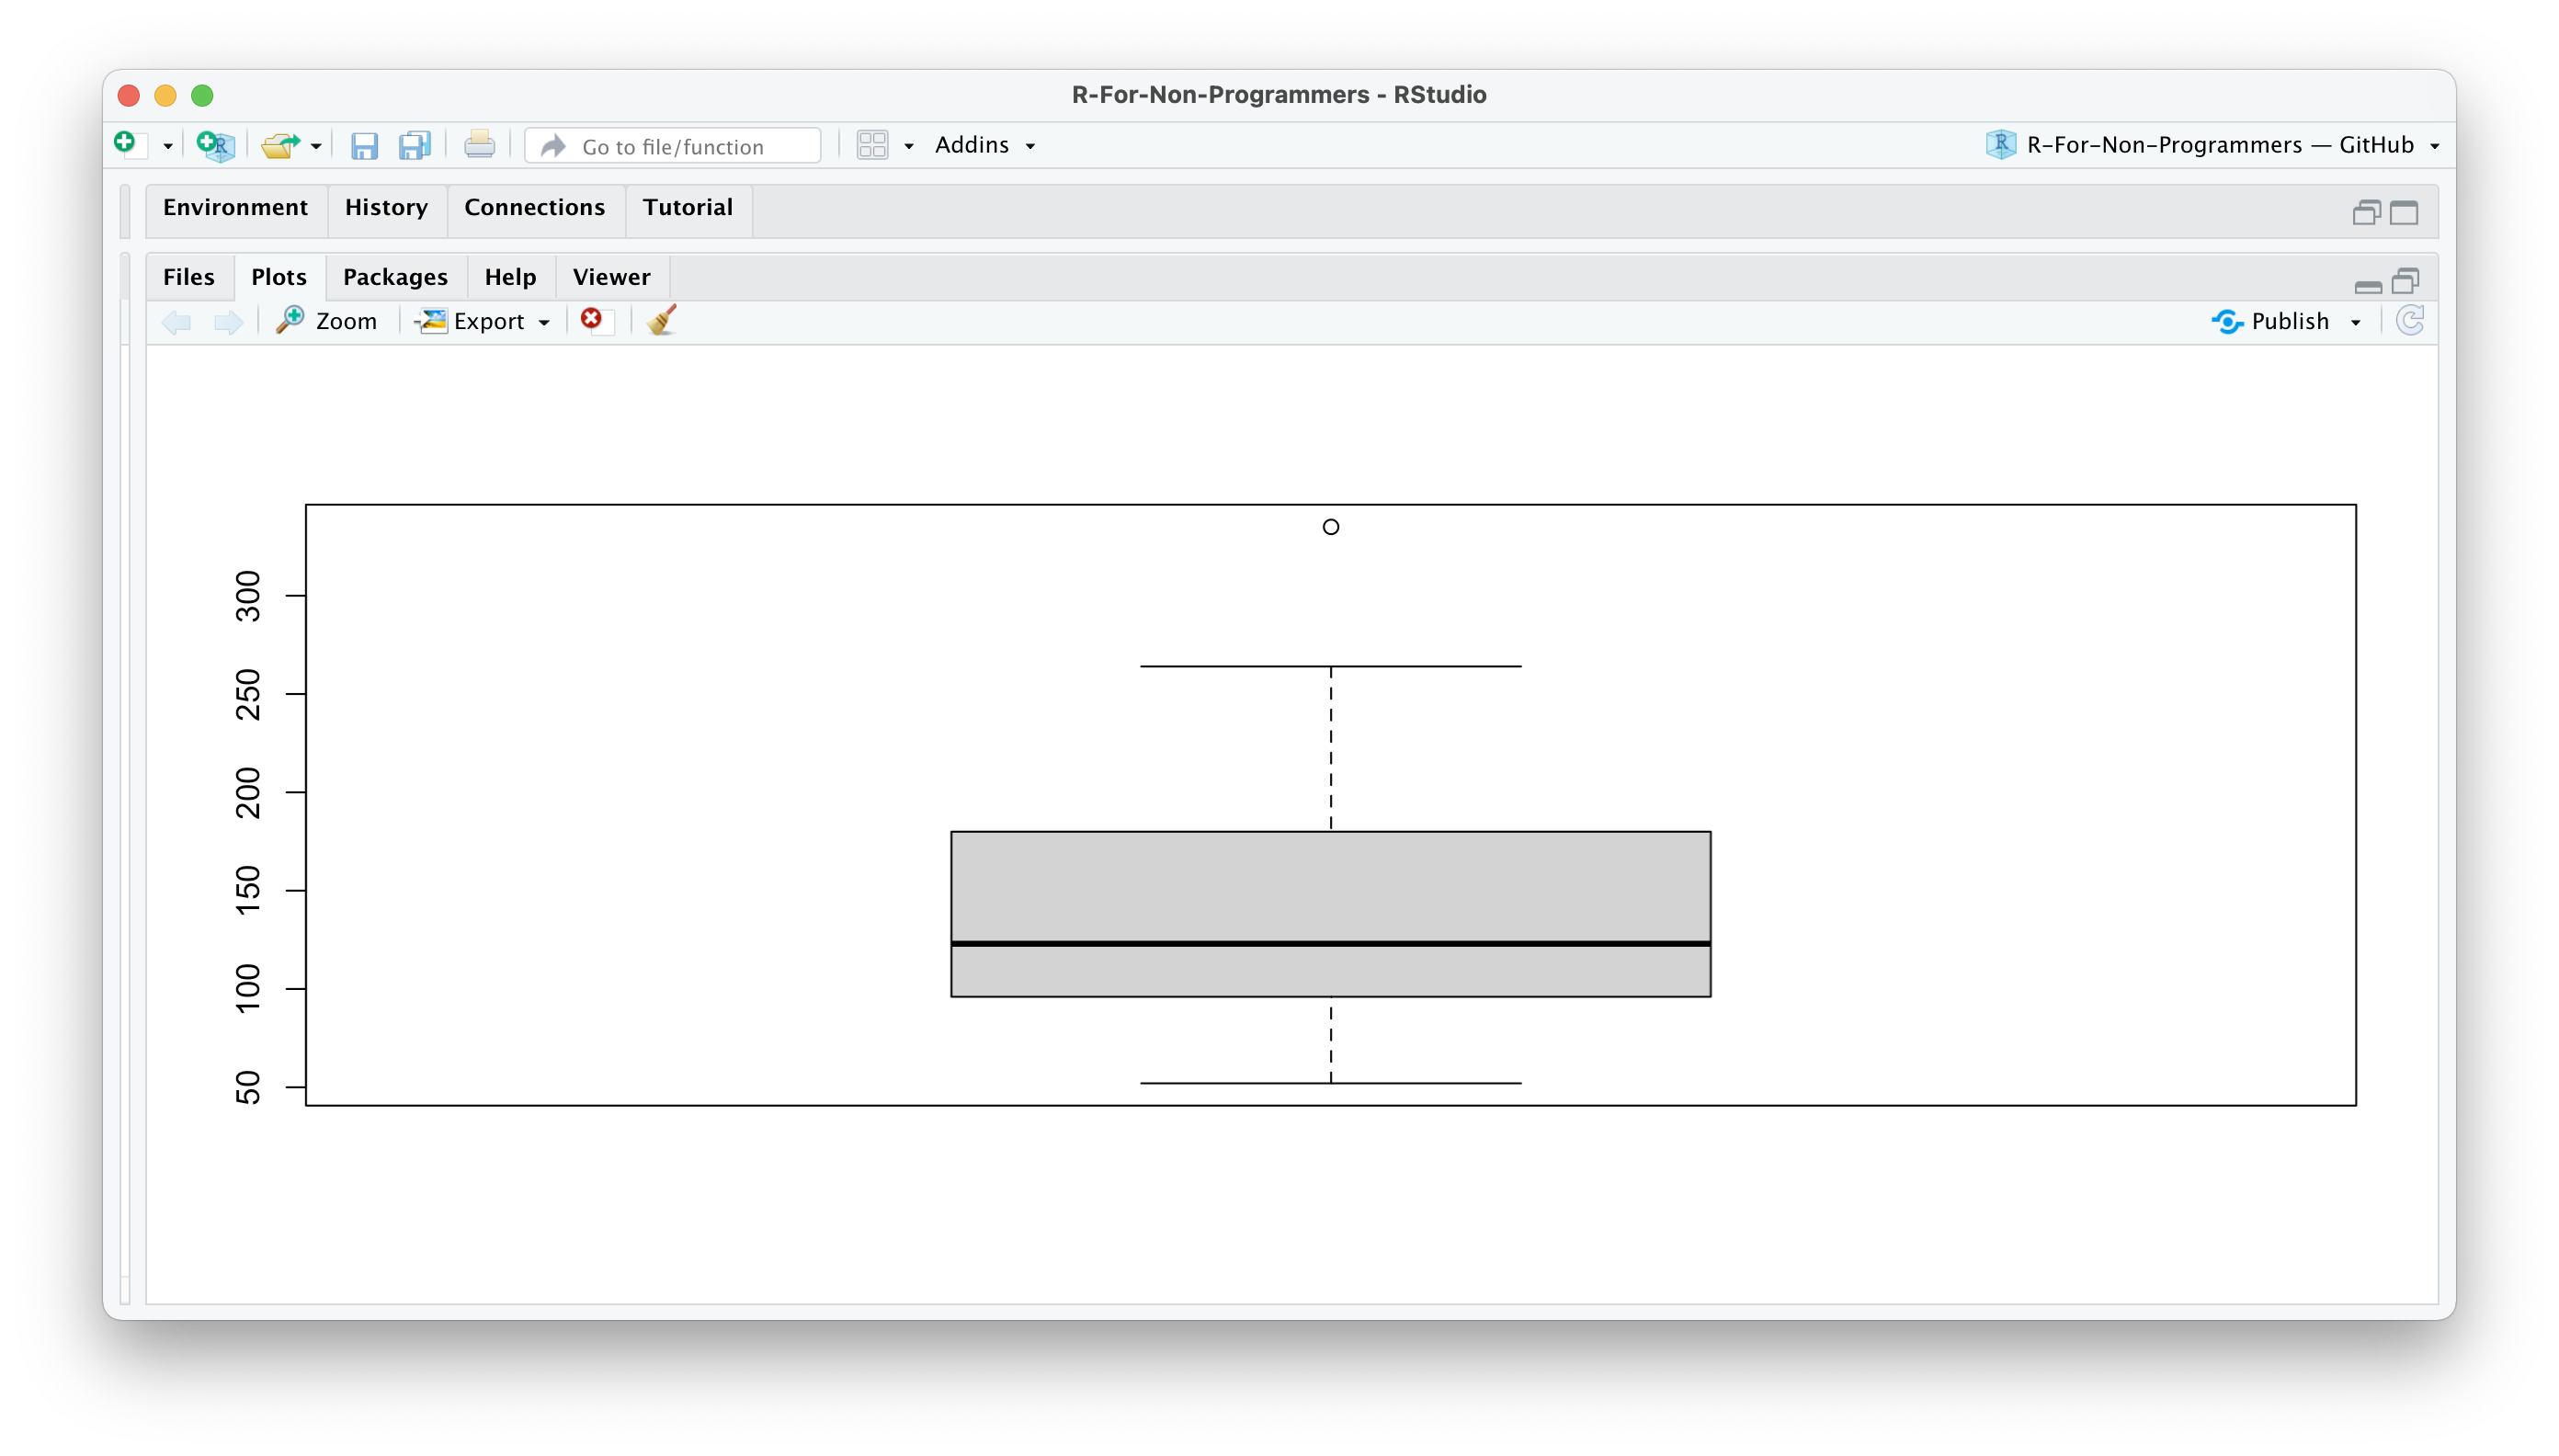
\includegraphics{images/chapter_04_img/05_files_plots_etc/02_rstudio_plots.png}

If you wish to delete the plot, you can click on the \texttt{red\ circle\ with\ a\ white\ x} symbol. This will delete the currently visible plot. If you wish to remove all plots from this pane, you can use the \texttt{broom}. There is also an option to export your plot and move back and forth between different plots.

Do not worry about the coding at this point. It will all make sense in the following chapters.

The next pane is called \emph{Packages}. Packages are additional tools you can import and use when performing your analysis. A frequent analogy people use to explain packages is your phone and the apps you install. Each package you download is equivalent to an app on your phone. It can enhance different aspects of working in \emph{R}, such as creating animated plots, using unique machine learning algorithms, or simply making your life easier by doing multiple computations with just one single line of code. You will learn more about \emph{R packages} in Chapter \ref{r-packages}.

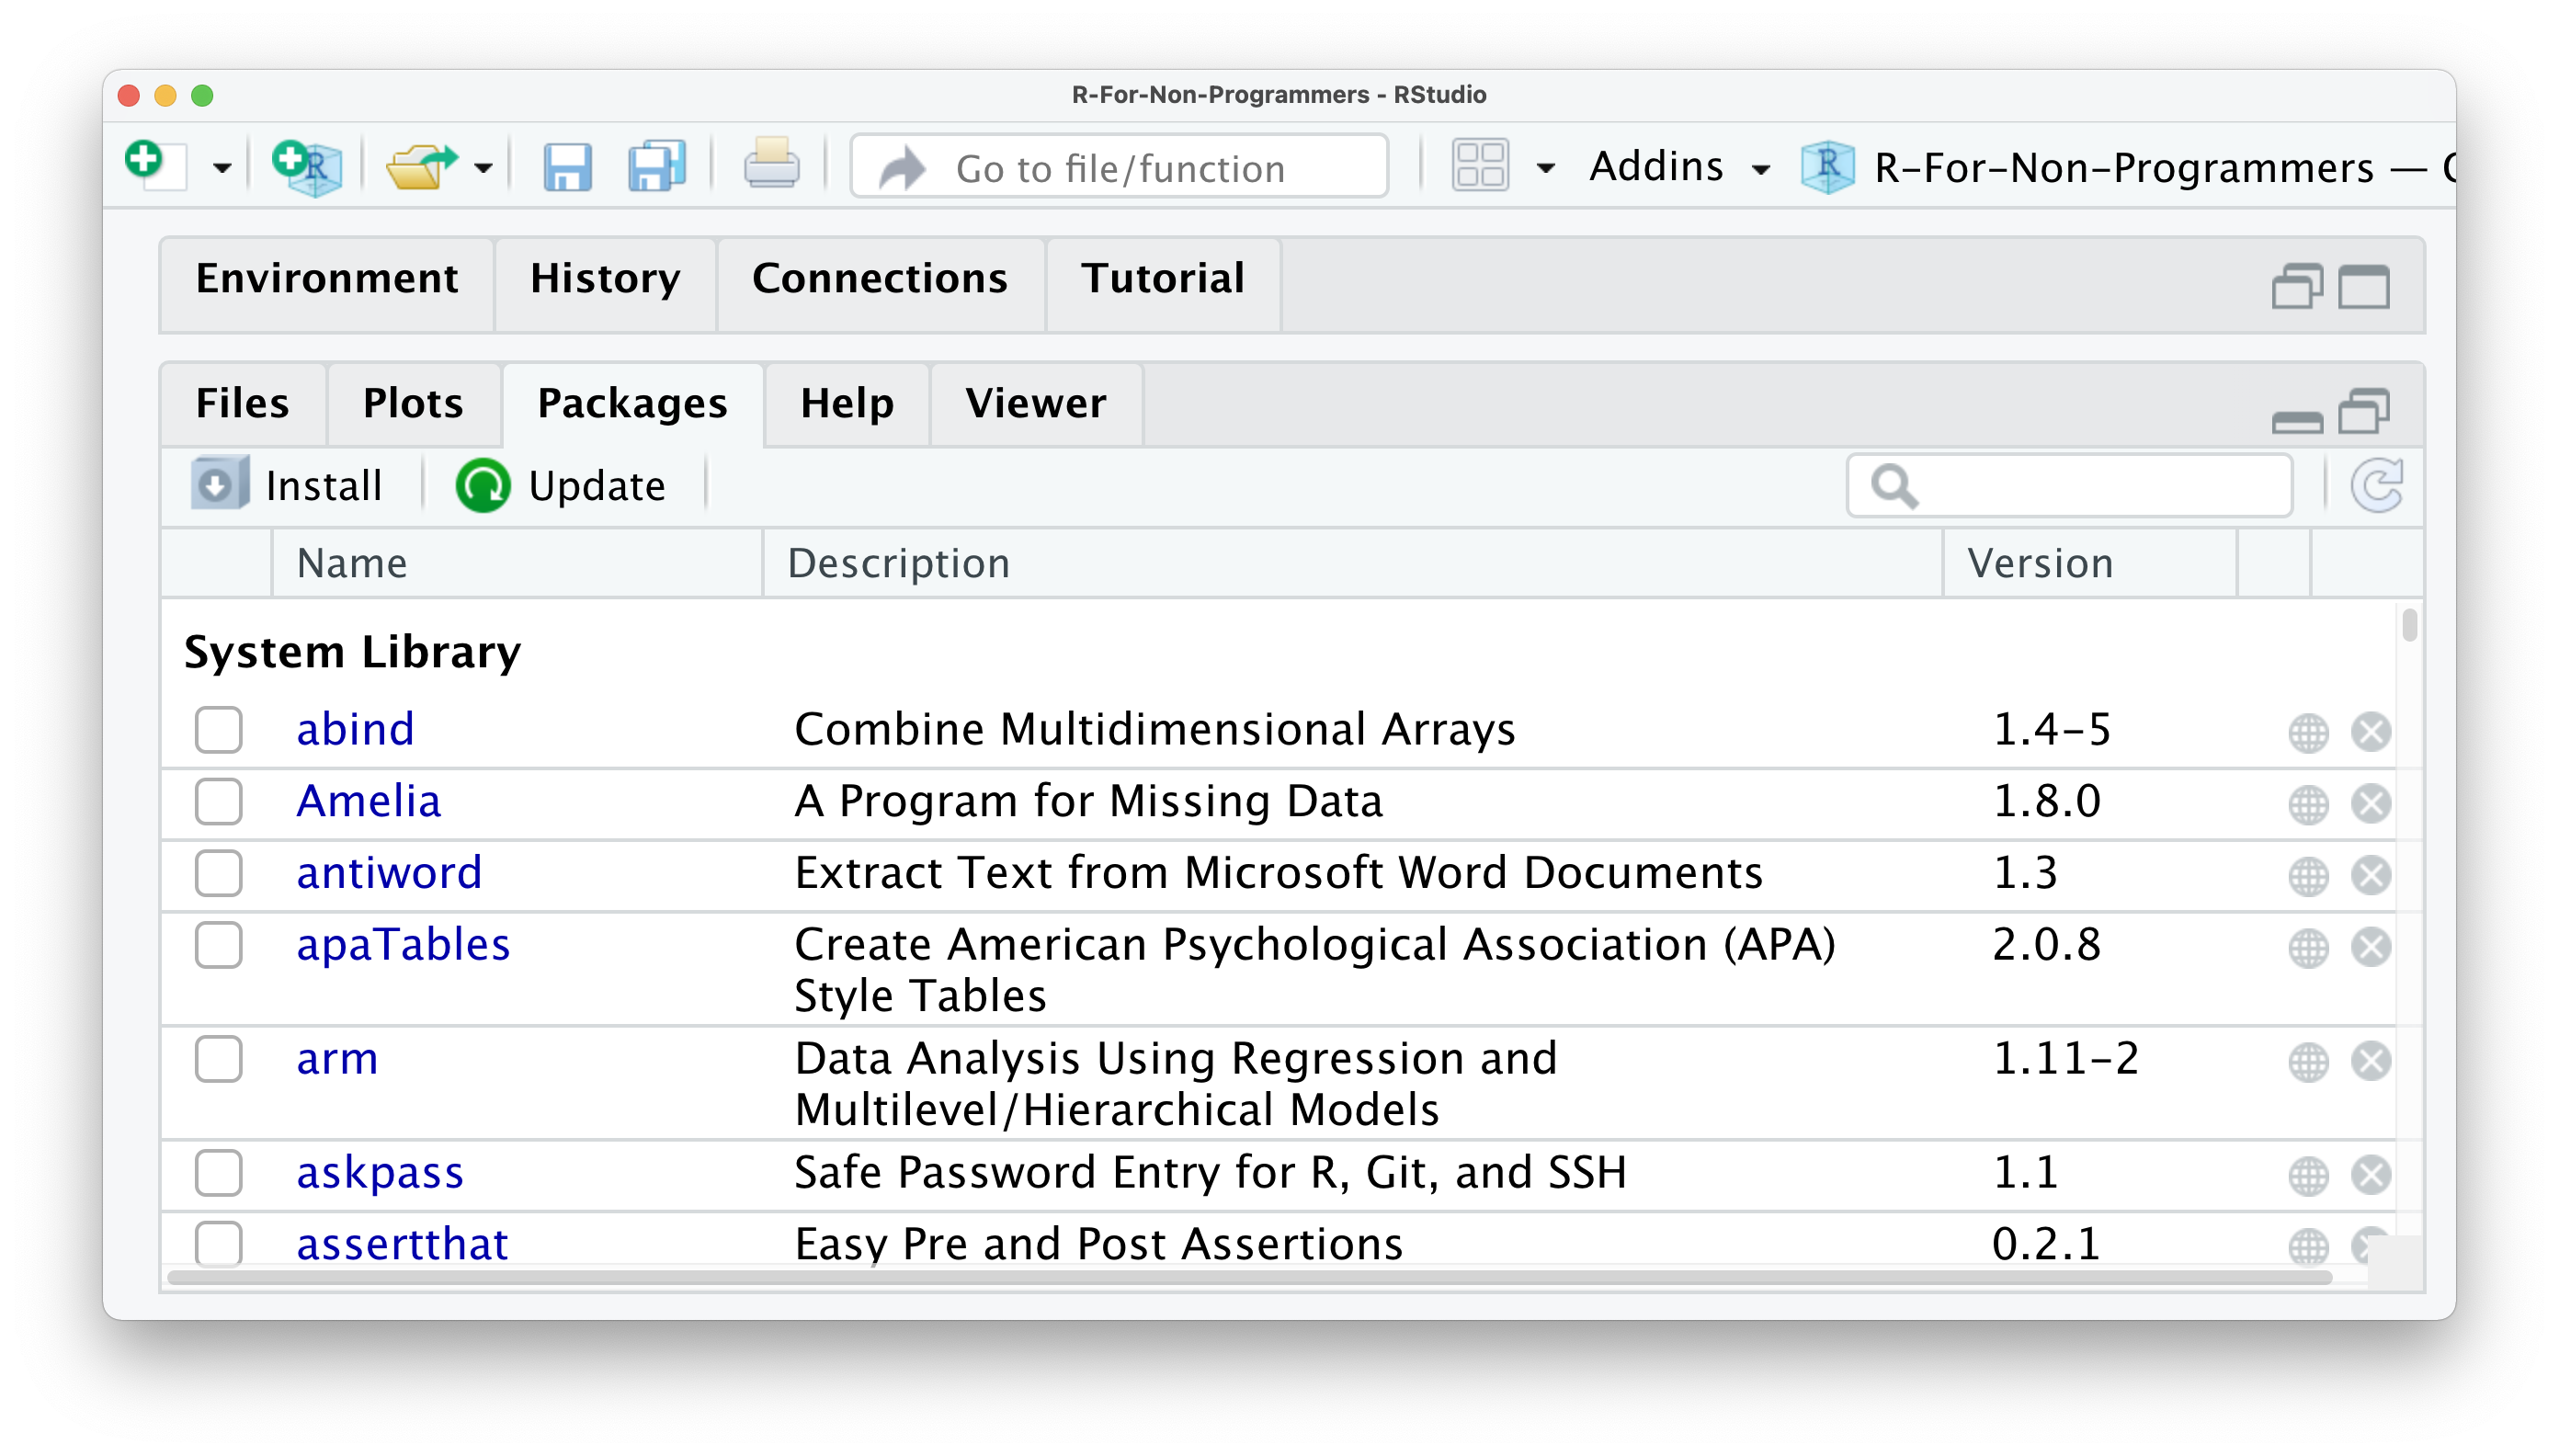
\includegraphics{images/chapter_04_img/05_files_plots_etc/03_rstudio_packages.png}

If you are in dire need of help, RStudio provides you with a \emph{Help} pane. You can search for specific topics, for example how certain computations work. The \emph{Help} pane also has documentation on different datasets that are included in \emph{R}, RStudio or \emph{R packages} you have installed.

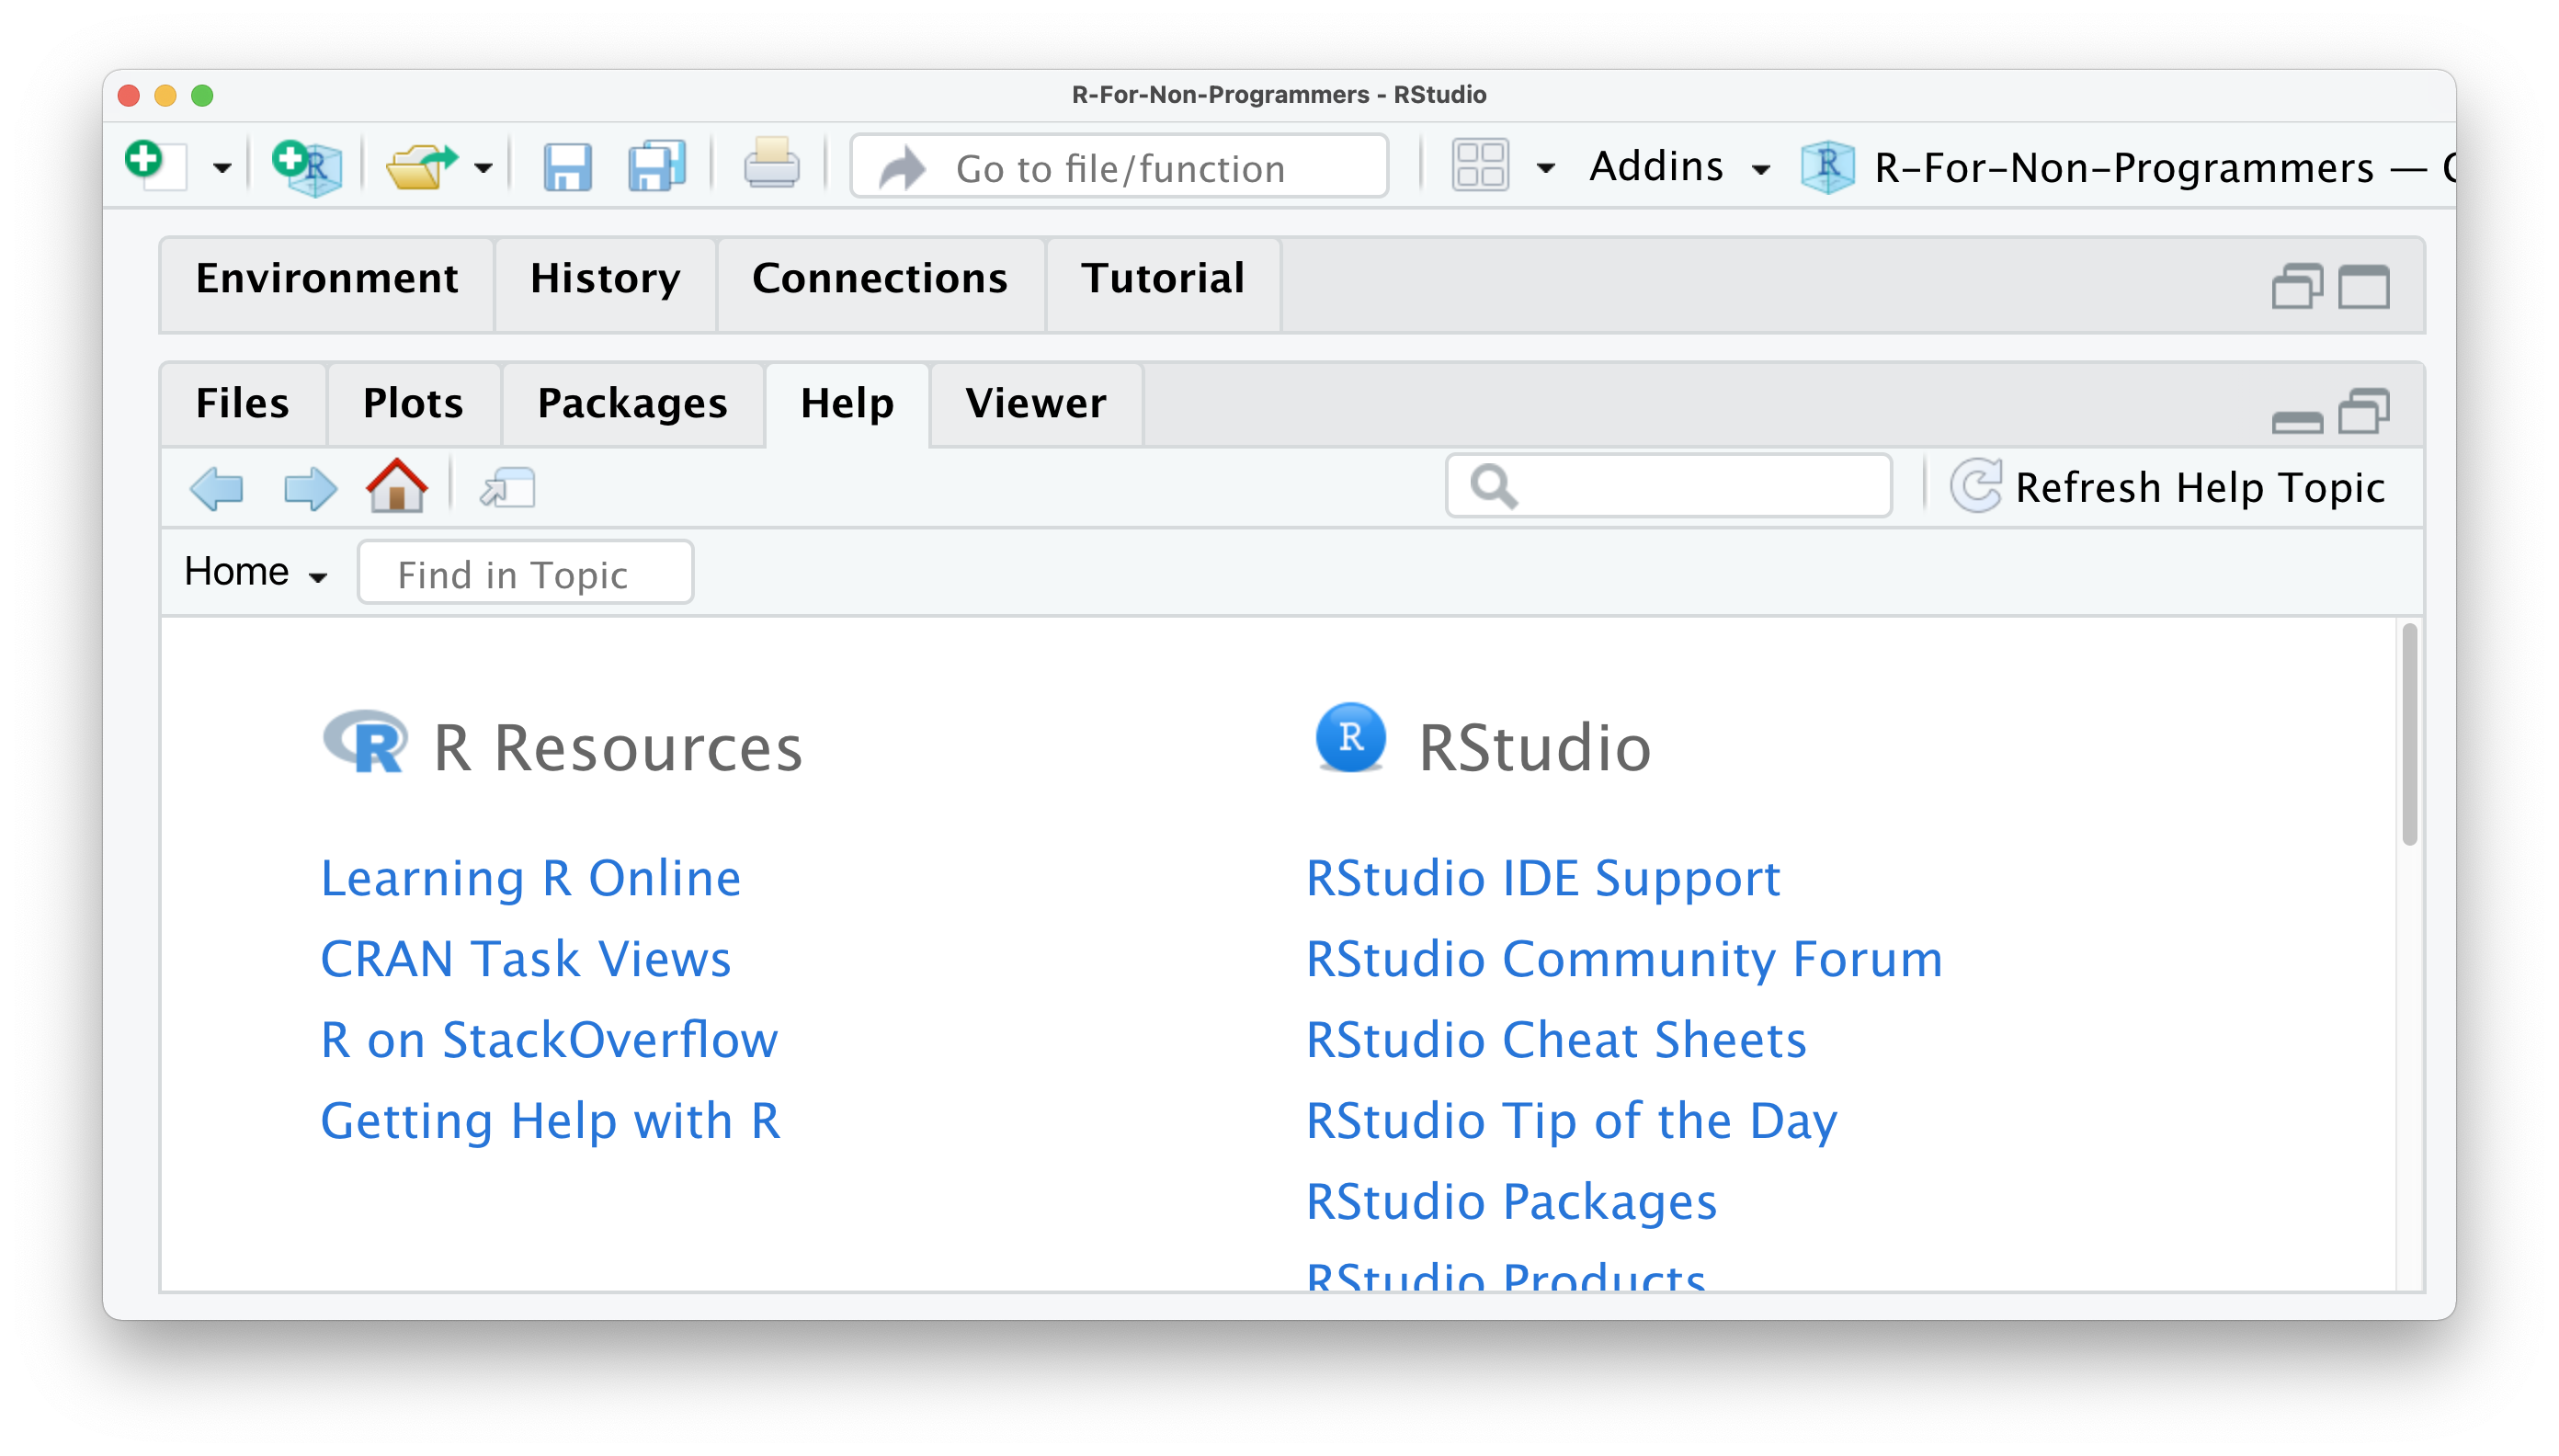
\includegraphics{images/chapter_04_img/05_files_plots_etc/04_rstudio_help.png}

So, for example, if you want to know what the \texttt{mtcars} dataset is, you can either use the search window in the \emph{Help} pane or, much easier, use a \texttt{?} in the console to search for it:

\begin{Shaded}
\begin{Highlighting}[]
\CommentTok{\# Type a \textquotesingle{}?\textquotesingle{} and immediately add the name to bring up helpful information.}

\NormalTok{?mtcars}
\end{Highlighting}
\end{Shaded}

This will open the \emph{Help} pane and give you more information about this dataset:

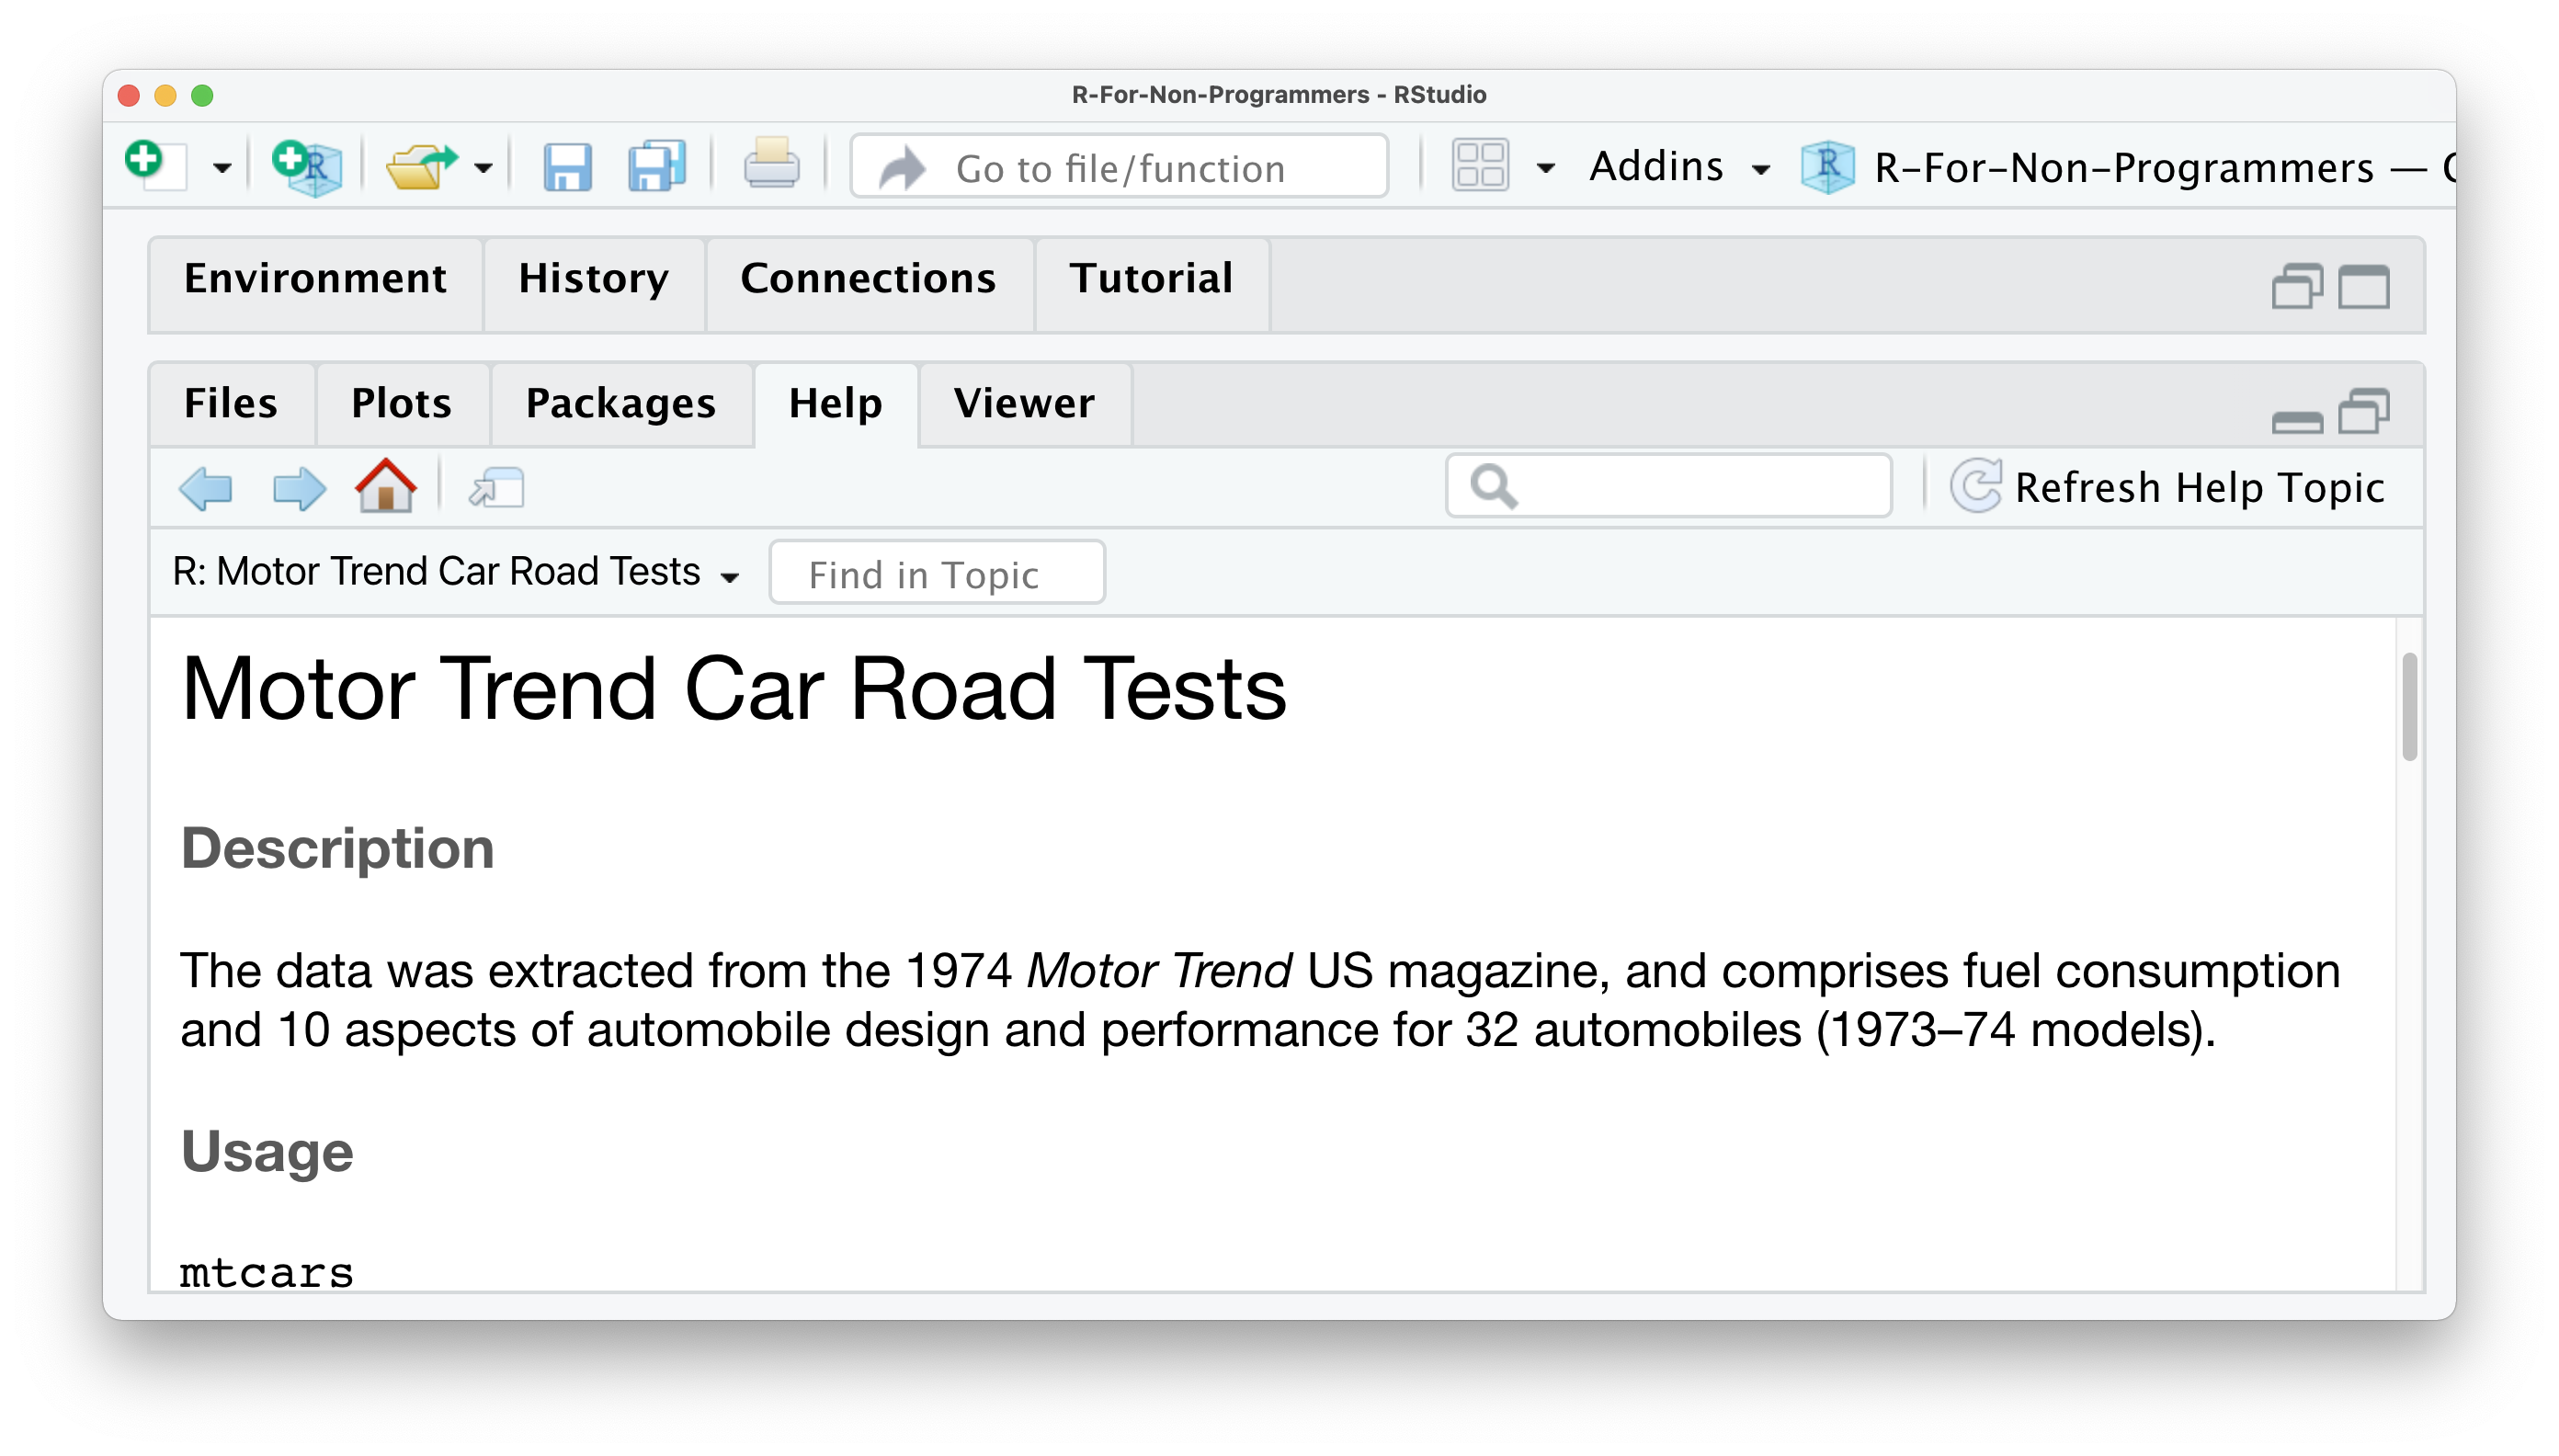
\includegraphics{images/chapter_04_img/05_files_plots_etc/04_rstudio_help_mtcars.png}

Lastly, we have the \emph{Viewer} pane. Not every data visualisation we create in R is a static image. You can create dynamic data visualisations or even websites with R. This type of content is displayed in the Viewer pane rather than in the Plots pane. Often these visualisations are based on HTML and other web-based programming languages. As such, it is easy to open them in your browser as well. However, in this book, we mainly focus on two-dimensional static plots, which are the ones you likely need most of the time, either for your assignments, thesis, or publication.

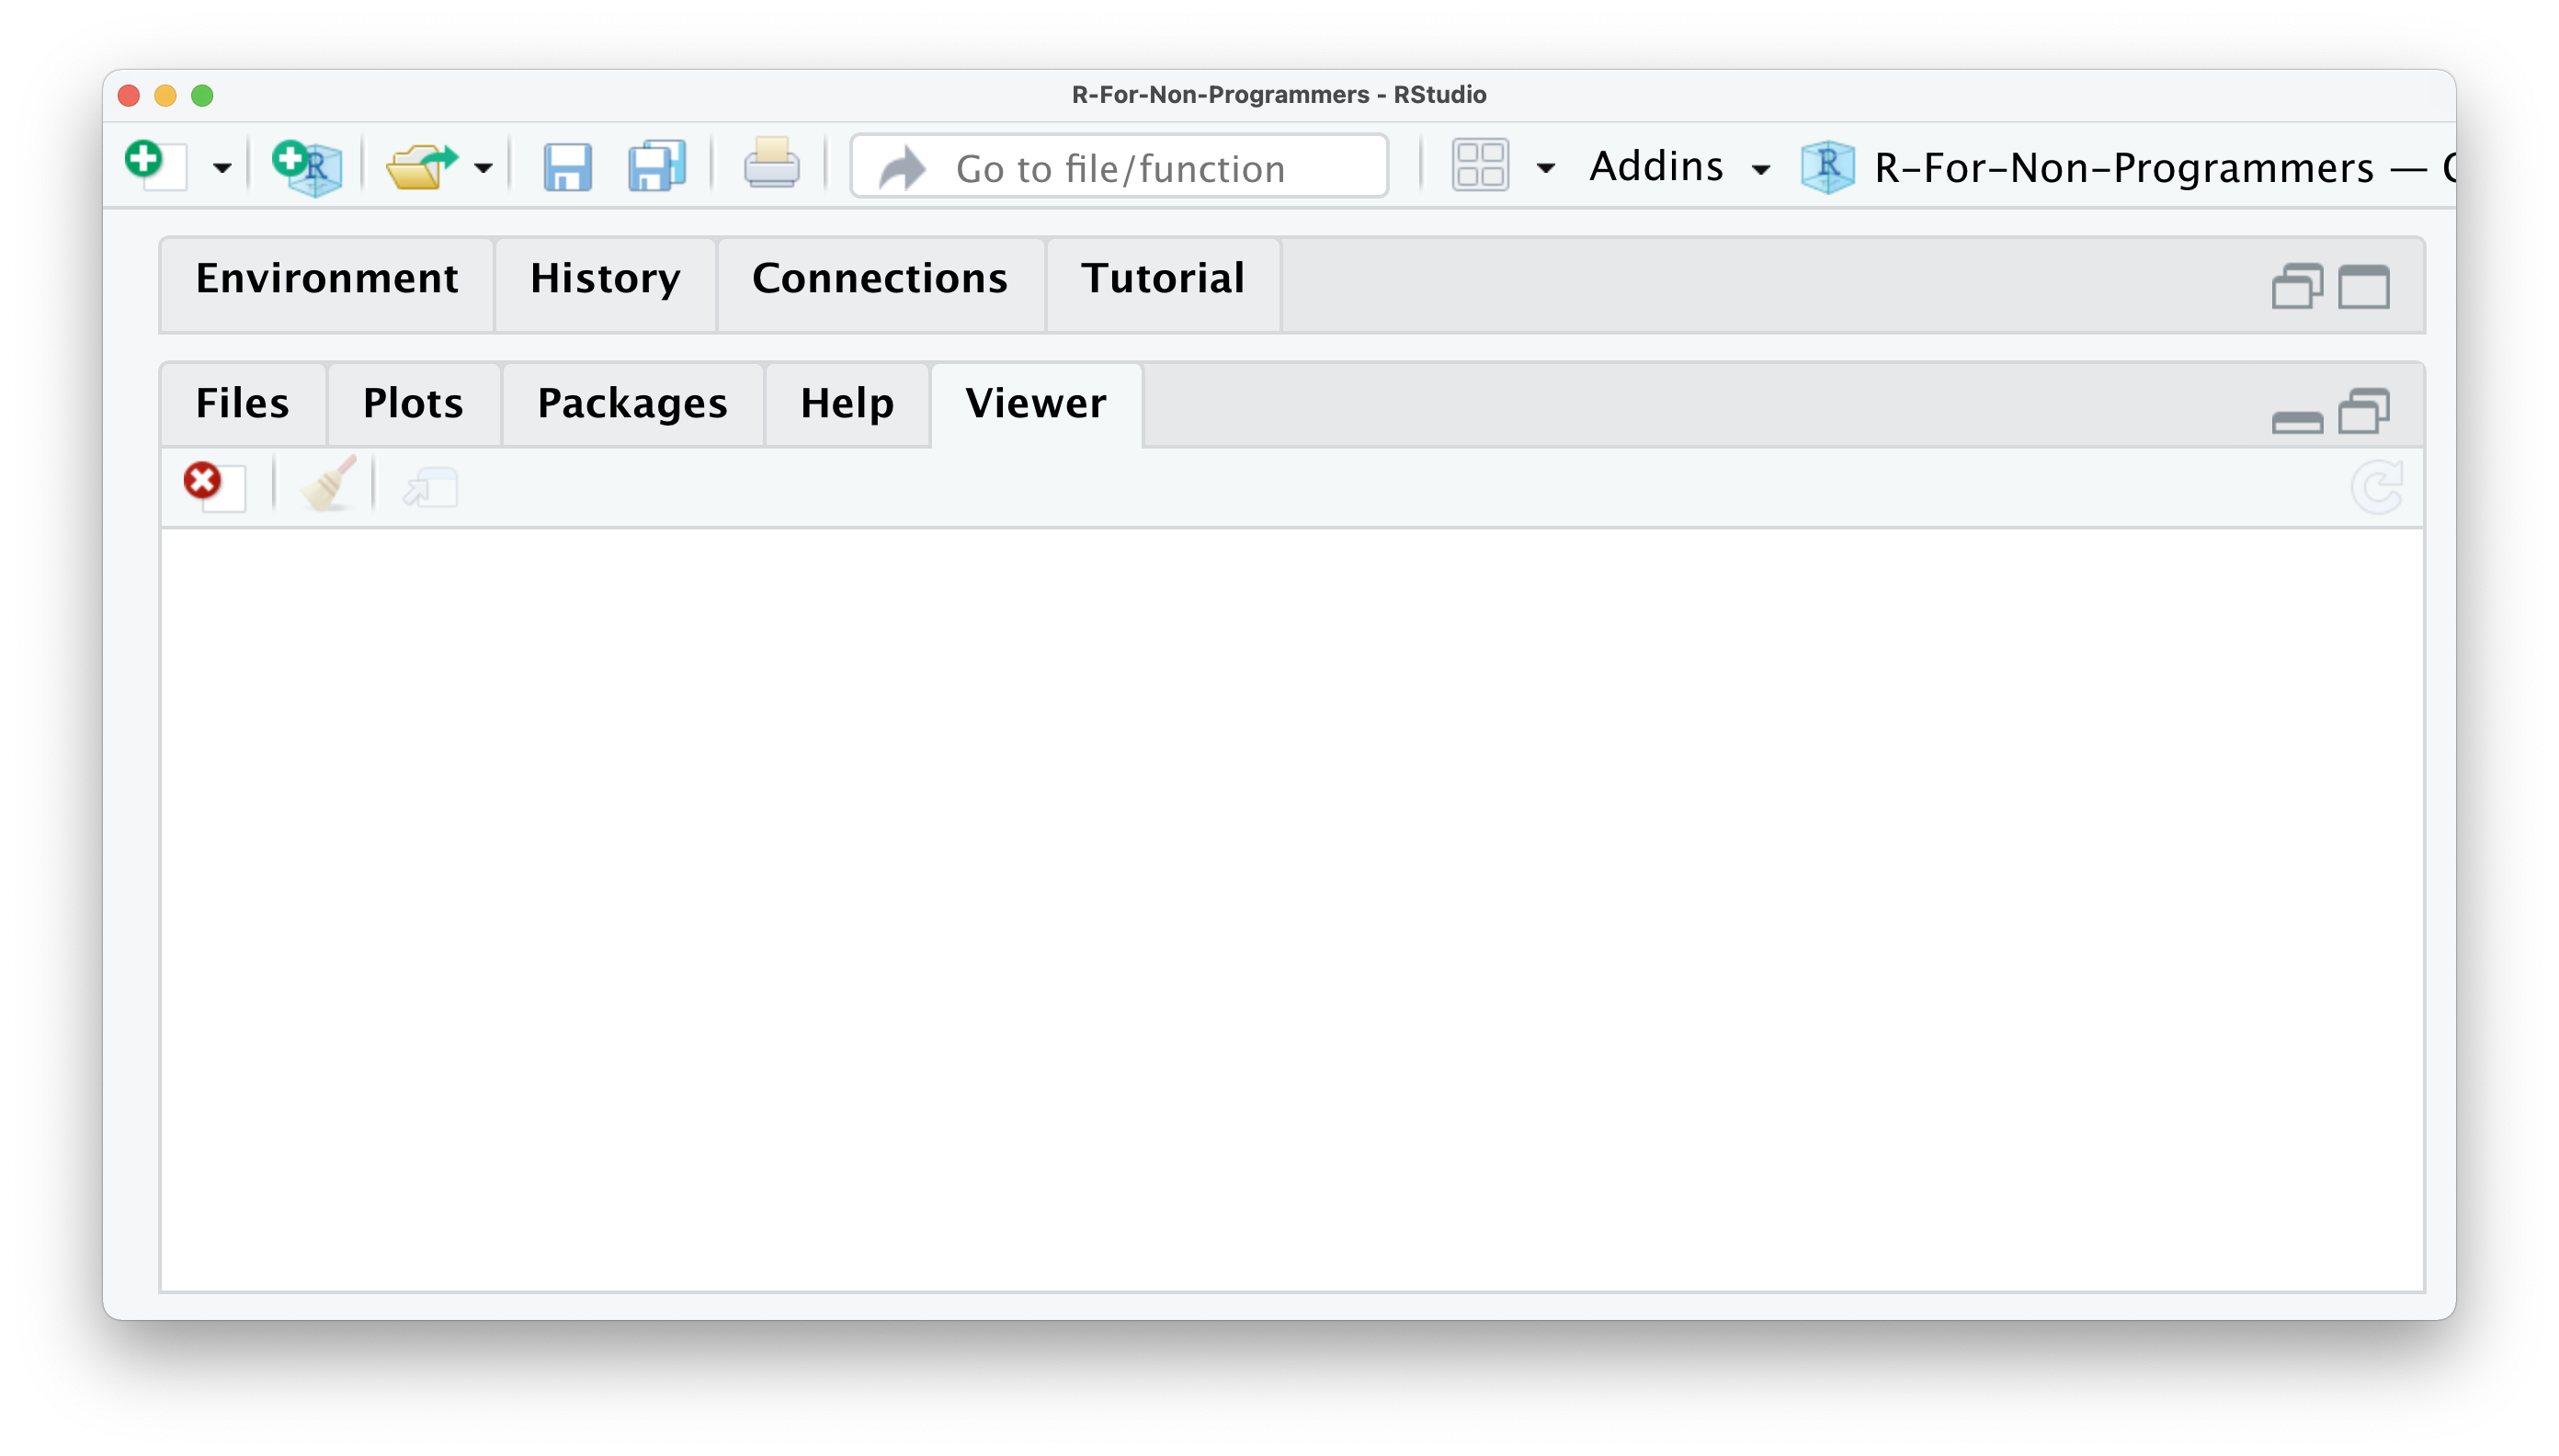
\includegraphics{images/chapter_04_img/05_files_plots_etc/05_rstudio_viewer.png}

\hypertarget{customise-your-user-interface}{%
\section{Customise your user interface}\label{customise-your-user-interface}}

As a last remark in this chapter, I would like to make you aware that you can modify each window. There are three basic adjustments you can make:

\begin{itemize}
\item
  Hide panes by clicking on the window symbol in the top right corner of each window,
\item
  Resize panes by dragging the border of a window horizontally or vertically, or
\item
  Add and remove panes by going to \texttt{RStudio\ \textgreater{}\ Preferences\ \textgreater{}\ Pane\ Layout}, or use the keyboard shortcut \texttt{⌘\ +\ ,} if you are on a Mac. There is, unfortunately no default shortcut for PC users.
\end{itemize}

\hypertarget{r-basics-the-very-fundamentals}{%
\chapter{R Basics: The very fundamentals}\label{r-basics-the-very-fundamentals}}

After a likely tedious installation of R and RStudio, as well as a somewhat detailed introduction to the RStudio interface, you are finally ready to `do' things. By `doing', I mean coding. The term `coding' in itself can instil fear in some of you, but you only need one skill to do it: Writing. As mentioned earlier, learning coding or programming means learning a new language. However, once you have the basic grammar down, you already can communicate quite a bit. In this section, we will explore the fundamentals of R. These build the foundation for everything that follows. After that, we dive right into some analysis.

\hypertarget{basic-computations-in-r}{%
\section{Basic computations in R}\label{basic-computations-in-r}}

The most basic computation you can do in R is arithmetic operations. In other words, addition, subtraction, multiplication, division, exponentiation and extraction of roots. In other words, R can be used like your pocket calculator, or more likely the one you have on your phone. For example, in Chapter \ref{the-console-window} we already performed an addition. Thus, it might not come as a surprise how their equivalents work in R. Let's take a look at the following examples:

\begin{Shaded}
\begin{Highlighting}[]
\CommentTok{\# Addition}
\DecValTok{10}\SpecialCharTok{+}\DecValTok{5}
\DocumentationTok{\#\# [1] 15}

\CommentTok{\# Subtraction}
\DecValTok{10{-}5}
\DocumentationTok{\#\# [1] 5}

\CommentTok{\# Multiplication}
\DecValTok{10}\SpecialCharTok{*}\DecValTok{5}
\DocumentationTok{\#\# [1] 50}

\CommentTok{\# Division}
\DecValTok{10}\SpecialCharTok{/}\DecValTok{5}
\DocumentationTok{\#\# [1] 2}

\CommentTok{\# Exponentiation}
\DecValTok{10}\SpecialCharTok{\^{}}\DecValTok{2}
\DocumentationTok{\#\# [1] 100}

\CommentTok{\# Square root}
\FunctionTok{sqrt}\NormalTok{(}\DecValTok{10}\NormalTok{)}
\DocumentationTok{\#\# [1] 3.162278}
\end{Highlighting}
\end{Shaded}

They all look fairly straightforward except for the extraction of roots. As you probably know, extracting the root would typically mean we use the symbol \(\sqrt{}\) on your calculator. To compute the square root in R, we have to use a function instead to perform the computation. So we first put the name of the function \texttt{sqrt} and then the value \texttt{10} within parenthesis \texttt{()}. This results in the following code: \texttt{sqrt(10)}. If we were to write this down in our report, we would write \(\sqrt[2]{10}\).

Functions are an essential part of R and programming in general. You will learn more about them in this chapter.Besides arithmetic operations, there are also logical queries you can perform. Logical queries always return either the value TRUE or FALSE. Here are some examples which make this clearer:

\begin{Shaded}
\begin{Highlighting}[]

\CommentTok{\#1 Is it TRUE or FALSE?}
\DecValTok{1} \SpecialCharTok{==} \DecValTok{1}
\DocumentationTok{\#\# [1] TRUE}

\CommentTok{\#2 Is 45 bigger than 55?}
\DecValTok{45} \SpecialCharTok{\textgreater{}} \DecValTok{55}
\DocumentationTok{\#\# [1] FALSE}

\CommentTok{\#3 Is 1982 bigger or equal to 1982?}
\DecValTok{1982} \SpecialCharTok{\textgreater{}=} \DecValTok{1982}
\DocumentationTok{\#\# [1] TRUE}

\CommentTok{\#4 Are these two words NOT the same?}
\StringTok{"Friends"} \SpecialCharTok{!=} \StringTok{"friends"}
\DocumentationTok{\#\# [1] TRUE}

\CommentTok{\#5 Are these sentences the same?}
\StringTok{"I love statistics"} \SpecialCharTok{==} \StringTok{"I love statistícs"}
\DocumentationTok{\#\# [1] FALSE}
\end{Highlighting}
\end{Shaded}

Reflecting on these examples, you might notice three important things:

\begin{enumerate}
\def\labelenumi{\arabic{enumi}.}
\tightlist
\item
  I used \texttt{==} instead of \texttt{=},
\item
  I can compare non-numerical values, i.e.~text, which is also known as \texttt{character\ values,} with each other,
\item
  The devil is in the details considering \#5.
\end{enumerate}

One of the most common mistakes of R novices is the confusion around the \texttt{==} and \texttt{=} notation. While \texttt{==} represents \texttt{equal\ to}, \texttt{=} is used to assign a value to an object (for more details on assignments see Chapter \ref{the-files-plots-packages-help-viewer-window}). However, in practice, most R programmers tend to avoid \texttt{=} since it can easily lead to confusion with \texttt{==}. As such, you can strike this one out of your R vocabulary for now.

There are many different logical operations you can perform. Table \ref{tab:logical-operators-r} lists the most frequently used logical operators for your reference. These will become important once we select only certain parts of our data for analysis, e.g.~only \texttt{female} participants.

\begin{longtable}[]{@{}ll@{}}
\caption{\label{tab:logical-operators-r} Logical Operators in R}\tabularnewline
\toprule
\begin{minipage}[b]{(\columnwidth - 1\tabcolsep) * \real{0.15}}\raggedright
Operator\strut
\end{minipage} & \begin{minipage}[b]{(\columnwidth - 1\tabcolsep) * \real{0.35}}\raggedright
Description\strut
\end{minipage}\tabularnewline
\midrule
\endfirsthead
\toprule
\begin{minipage}[b]{(\columnwidth - 1\tabcolsep) * \real{0.15}}\raggedright
Operator\strut
\end{minipage} & \begin{minipage}[b]{(\columnwidth - 1\tabcolsep) * \real{0.35}}\raggedright
Description\strut
\end{minipage}\tabularnewline
\midrule
\endhead
\begin{minipage}[t]{(\columnwidth - 1\tabcolsep) * \real{0.15}}\raggedright
==\strut
\end{minipage} & \begin{minipage}[t]{(\columnwidth - 1\tabcolsep) * \real{0.35}}\raggedright
is equal to\strut
\end{minipage}\tabularnewline
\begin{minipage}[t]{(\columnwidth - 1\tabcolsep) * \real{0.15}}\raggedright
\textgreater=\strut
\end{minipage} & \begin{minipage}[t]{(\columnwidth - 1\tabcolsep) * \real{0.35}}\raggedright
is bigger or equal to\strut
\end{minipage}\tabularnewline
\begin{minipage}[t]{(\columnwidth - 1\tabcolsep) * \real{0.15}}\raggedright
\textless=\strut
\end{minipage} & \begin{minipage}[t]{(\columnwidth - 1\tabcolsep) * \real{0.35}}\raggedright
is smaller of equal to\strut
\end{minipage}\tabularnewline
\begin{minipage}[t]{(\columnwidth - 1\tabcolsep) * \real{0.15}}\raggedright
!=\strut
\end{minipage} & \begin{minipage}[t]{(\columnwidth - 1\tabcolsep) * \real{0.35}}\raggedright
is not equal to\strut
\end{minipage}\tabularnewline
\begin{minipage}[t]{(\columnwidth - 1\tabcolsep) * \real{0.15}}\raggedright
a \textbar{} b\strut
\end{minipage} & \begin{minipage}[t]{(\columnwidth - 1\tabcolsep) * \real{0.35}}\raggedright
a or b\strut
\end{minipage}\tabularnewline
\begin{minipage}[t]{(\columnwidth - 1\tabcolsep) * \real{0.15}}\raggedright
a \& b\strut
\end{minipage} & \begin{minipage}[t]{(\columnwidth - 1\tabcolsep) * \real{0.35}}\raggedright
a and b\strut
\end{minipage}\tabularnewline
\begin{minipage}[t]{(\columnwidth - 1\tabcolsep) * \real{0.15}}\raggedright
!a\strut
\end{minipage} & \begin{minipage}[t]{(\columnwidth - 1\tabcolsep) * \real{0.35}}\raggedright
is not a\strut
\end{minipage}\tabularnewline
\bottomrule
\end{longtable}

\hypertarget{assigning-values-to-objects-}{%
\section{Assigning values to objects: `\textless-'}\label{assigning-values-to-objects-}}

Another common task you will perform is assigning values to an object. An object can be many different things:

\begin{itemize}
\item
  a dataset,
\item
  the results of a computation,
\item
  a plot,
\item
  a series of numbers,
\item
  a list of names,
\item
  a function,
\item
  etc.
\end{itemize}

In short, an object is an umbrella term for many different things which form part of your data analysis. For example, objects are handy when storing results that you want to process further in later analytical steps. Let's have a look at an example.

\begin{Shaded}
\begin{Highlighting}[]
\CommentTok{\# I have a friend called "Fiona"}
\NormalTok{friends }\OtherTok{\textless{}{-}} \StringTok{"Fiona"}
\end{Highlighting}
\end{Shaded}

In this example, I created an object called \texttt{friends} and added \texttt{"Fiona"} to it. Remember, because \texttt{"Fiona"} represents a \texttt{string}, we need \texttt{""}. So, if you wanted to read this line of code, you would say, `\texttt{friends} gets the value \texttt{"Fiona"}'. Alternatively, you could also say `\texttt{"Fiona"} is assigned to \texttt{friends}'.

If you look into your environment pane, you will find the object we just created. You can see it carries the value \texttt{"Fiona"}. We can also print values of an object in the console by simply typing the name of the object \texttt{friends} and hit \texttt{Return\ ↵}.

\begin{Shaded}
\begin{Highlighting}[]
\CommentTok{\# Who are my friends?}
\NormalTok{friends}
\end{Highlighting}
\end{Shaded}

\begin{verbatim}
## [1] "Fiona"
\end{verbatim}

Sadly, it seems I only have one friend. Luckily we can add some more, not the least to make me feel less lonely. To create objects with multiple values, we can use the function \texttt{c()}, which stands for `concatenate'. The \citet{concatenate-2021} define this word as follows:

\begin{quote}
`\textbf{\emph{concatenate}}',

to put things together as a connected series
\end{quote}

Let's concatenate some more friends into our \texttt{friends} object.

\begin{Shaded}
\begin{Highlighting}[]
\CommentTok{\# Adding some more friends to my life}
\NormalTok{friends }\OtherTok{\textless{}{-}} \FunctionTok{c}\NormalTok{(}\StringTok{"Fiona"}\NormalTok{, }\StringTok{"Ida"}\NormalTok{, }\StringTok{"Lukas"}\NormalTok{, }\StringTok{"Georg"}\NormalTok{, }\StringTok{"Daniel"}\NormalTok{, }\StringTok{"Pavel"}\NormalTok{, }\StringTok{"Tigger"}\NormalTok{)}

\CommentTok{\# Here are all my friends}
\NormalTok{friends}
\DocumentationTok{\#\# [1] "Fiona"  "Ida"    "Lukas"  "Georg"  "Daniel" "Pavel"  "Tigger"}
\end{Highlighting}
\end{Shaded}

To concatenate values into a single object, we need to use a comma \texttt{,} to separate each value. Otherwise, R will report an error back.

\begin{Shaded}
\begin{Highlighting}[]
\NormalTok{friends }\OtherTok{\textless{}{-}} \FunctionTok{c}\NormalTok{(}\StringTok{"Fiona"} \StringTok{"Ida"}\NormalTok{)}
\DocumentationTok{\#\# Error: \textless{}text\textgreater{}:1:22: unexpected string constant}
\DocumentationTok{\#\# 1: friends \textless{}{-} c("Fiona" "Ida"}
\DocumentationTok{\#\#                          \^{}}
\end{Highlighting}
\end{Shaded}

R's error messages tend to be very useful and give meaningful clues to what went wrong. In this case, we can see that something `unexpected' happen, and it shows where our mistake is.

You can also concatenate numbers, and if you add \texttt{()} around it, you can automatically print the content of the object to the console. Thus, \texttt{(milestones\_of\_my\_life\ \textless{}-\ c(1982,\ 2006,\ 2011,\ 2018,\ 2020))} is the same as \texttt{milestones\_of\_my\_life\ \textless{}-\ c(1982,\ 2006,\ 2011,\ 2018,\ 2020)} followed by \texttt{milestones\_of\_my\_life}. The following examples illustrate this.

\begin{Shaded}
\begin{Highlighting}[]
\CommentTok{\# Important years in my life}
\NormalTok{milestones\_of\_my\_life }\OtherTok{\textless{}{-}} \FunctionTok{c}\NormalTok{(}\DecValTok{1982}\NormalTok{, }\DecValTok{2006}\NormalTok{, }\DecValTok{2011}\NormalTok{, }\DecValTok{2018}\NormalTok{, }\DecValTok{2020}\NormalTok{)}
\NormalTok{milestones\_of\_my\_life}
\DocumentationTok{\#\# [1] 1982 2006 2011 2018 2020}

\CommentTok{\# The same as above, but we don\textquotesingle{}t need the second line of code}
\NormalTok{(milestones\_of\_my\_life }\OtherTok{\textless{}{-}} \FunctionTok{c}\NormalTok{(}\DecValTok{1982}\NormalTok{, }\DecValTok{2006}\NormalTok{, }\DecValTok{2011}\NormalTok{, }\DecValTok{2018}\NormalTok{, }\DecValTok{2020}\NormalTok{))}
\DocumentationTok{\#\# [1] 1982 2006 2011 2018 2020}
\end{Highlighting}
\end{Shaded}

Finally, we can also concatenate numbers and character values into one object:

\begin{Shaded}
\begin{Highlighting}[]
\NormalTok{(names\_and\_years }\OtherTok{\textless{}{-}} \FunctionTok{c}\NormalTok{(}\StringTok{"Fiona"}\NormalTok{, }\DecValTok{1988}\NormalTok{, }\StringTok{"Daniel"}\NormalTok{, }\DecValTok{1982}\NormalTok{))}
\DocumentationTok{\#\# [1] "Fiona"  "1988"   "Daniel" "1982"}
\end{Highlighting}
\end{Shaded}

This last example is not necessarily something I would recommend to do, because it likely leads to undesirable outcomes. If you look into your environment pane you currently have three objects: \texttt{friends}, \texttt{milestones\_of\_my\_life}, and \texttt{names\_and\_years}.

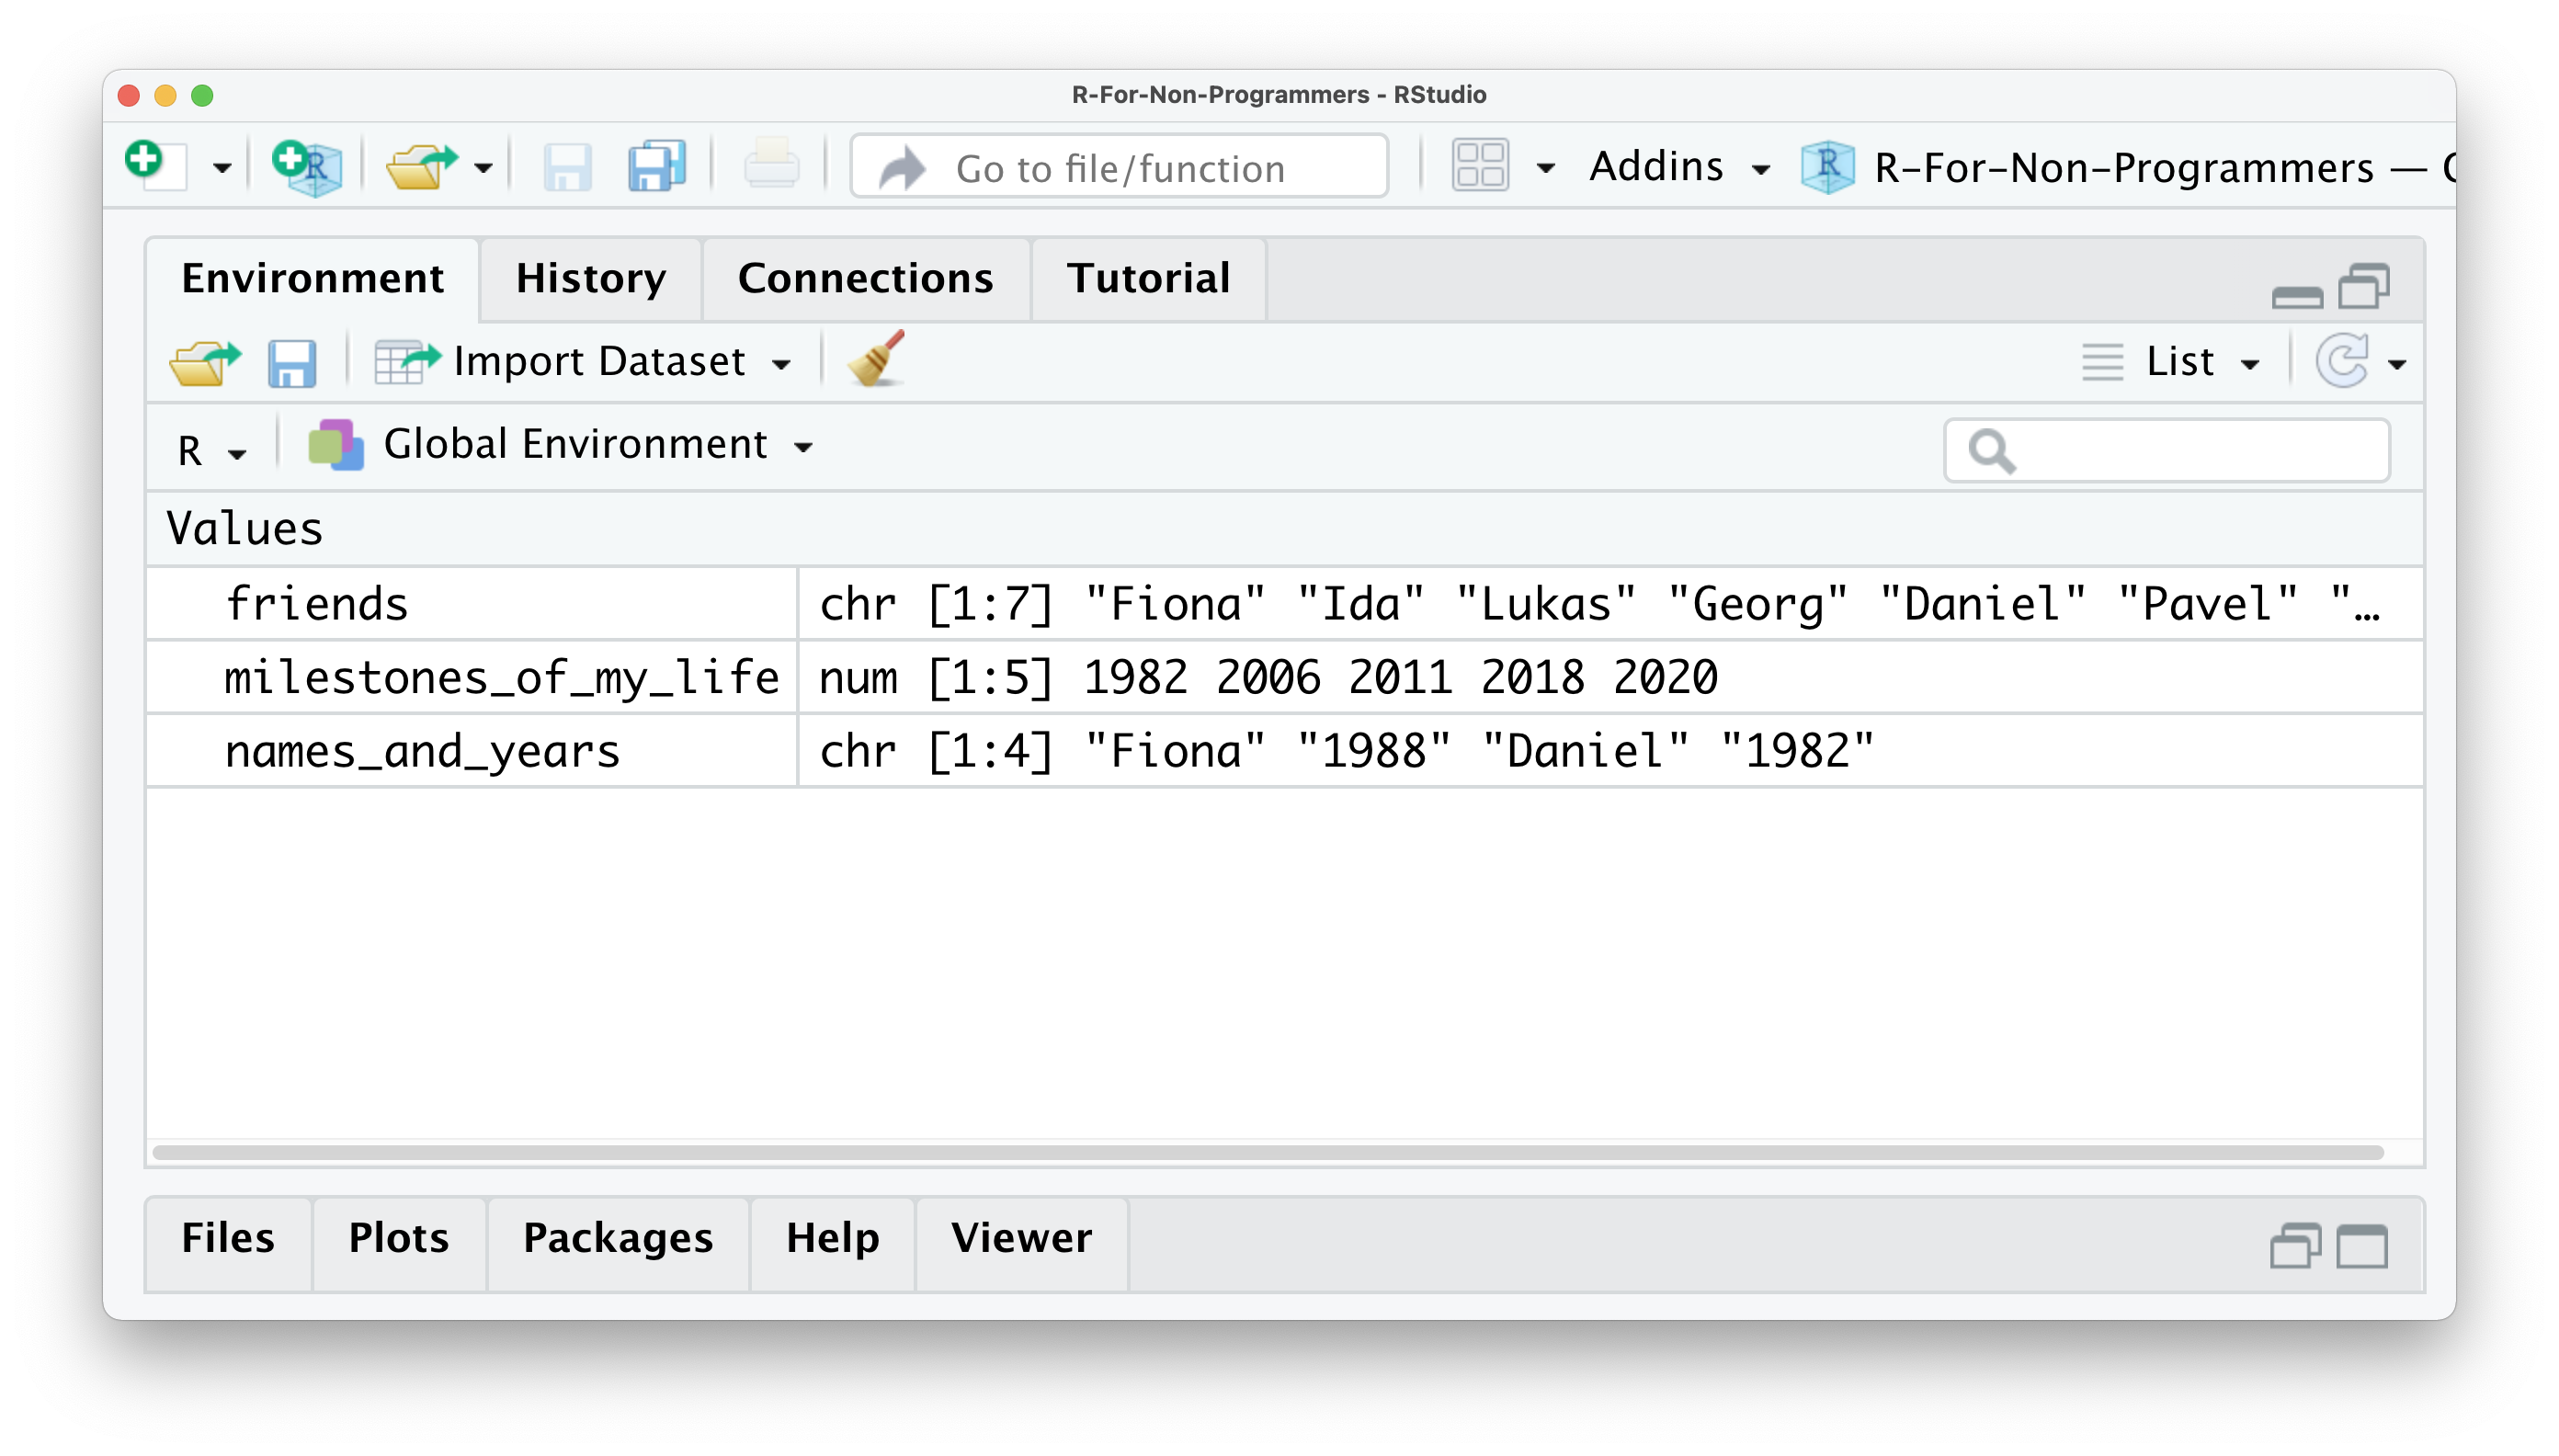
\includegraphics{images/chapter_05_img/01_basic_computation_environment_objects.png}

The \texttt{friends} object shows that all the values inside the object are classified as \texttt{chr}, which denominates \texttt{character}. In this case, this is correct because it only includes the names of my friends. On the other hand, the object \texttt{milestones\_of\_my\_life} only includes \texttt{numeric} values, and therefore it says \texttt{num} in the environment pane. However, for the object \texttt{names\_and\_years} we know we want to have \texttt{numeric} and \texttt{character} values included. Still, R recognises them as \texttt{character} values only because values inside objects are meant to be of the same type.

Consequently, mixing different types of data (as explained in Chapter @ref()) into one object is likely a bad idea. This is especially true if you want to use the numeric values for computation. In short: ensure your objects are all of the same data type.

There is an exception to this rule. `Of course', you might say. There is one object that can have values of different types: list. As the name indicates, a list object holds several items. These items are usually other objects. In the spirit of `\href{https://www.imdb.com/title/tt1375666/?ref_=ext_shr_lnk}{Inception}', you can have lists inside lists, which contain more objects.

Let's create a list called \texttt{x\_files} using the \texttt{list} function and place all our objects inside.

\begin{Shaded}
\begin{Highlighting}[]
\CommentTok{\# This creates our list of objects}
\NormalTok{x\_files }\OtherTok{\textless{}{-}} \FunctionTok{list}\NormalTok{(friends,}
\NormalTok{               milestones\_of\_my\_life,}
\NormalTok{               names\_and\_years)}

\CommentTok{\# Let\textquotesingle{}s have a look what is hidden inside the x\_files}
\NormalTok{x\_files}
\DocumentationTok{\#\# [[1]]}
\DocumentationTok{\#\# [1] "Fiona"  "Ida"    "Lukas"  "Georg"  "Daniel" "Pavel"  "Tigger"}
\DocumentationTok{\#\# }
\DocumentationTok{\#\# [[2]]}
\DocumentationTok{\#\# [1] 1982 2006 2011 2018 2020}
\DocumentationTok{\#\# }
\DocumentationTok{\#\# [[3]]}
\DocumentationTok{\#\# [1] "Fiona"  "1988"   "Daniel" "1982"}
\end{Highlighting}
\end{Shaded}

You will notice in this example that I do not use \texttt{""} for each value in the list. This is because \texttt{friends} is not a character I put into the list, but an object. When we refer to objects we do not need the quotation marks.

We will encounter lists quite frequently when we perform our analysis. Some functions return the results in the format of lists. This can be very helpful, because otherwise our environment pane will be littered with objects, but we would not necessarily know how they relate to each other or worse, to which analysis they belong. Looking at the list item in the environment page, you can see that the object \texttt{x\_files} is classified as a \texttt{List\ of\ 3} and if you click on the blue icon, you can inspect the different objects inside.

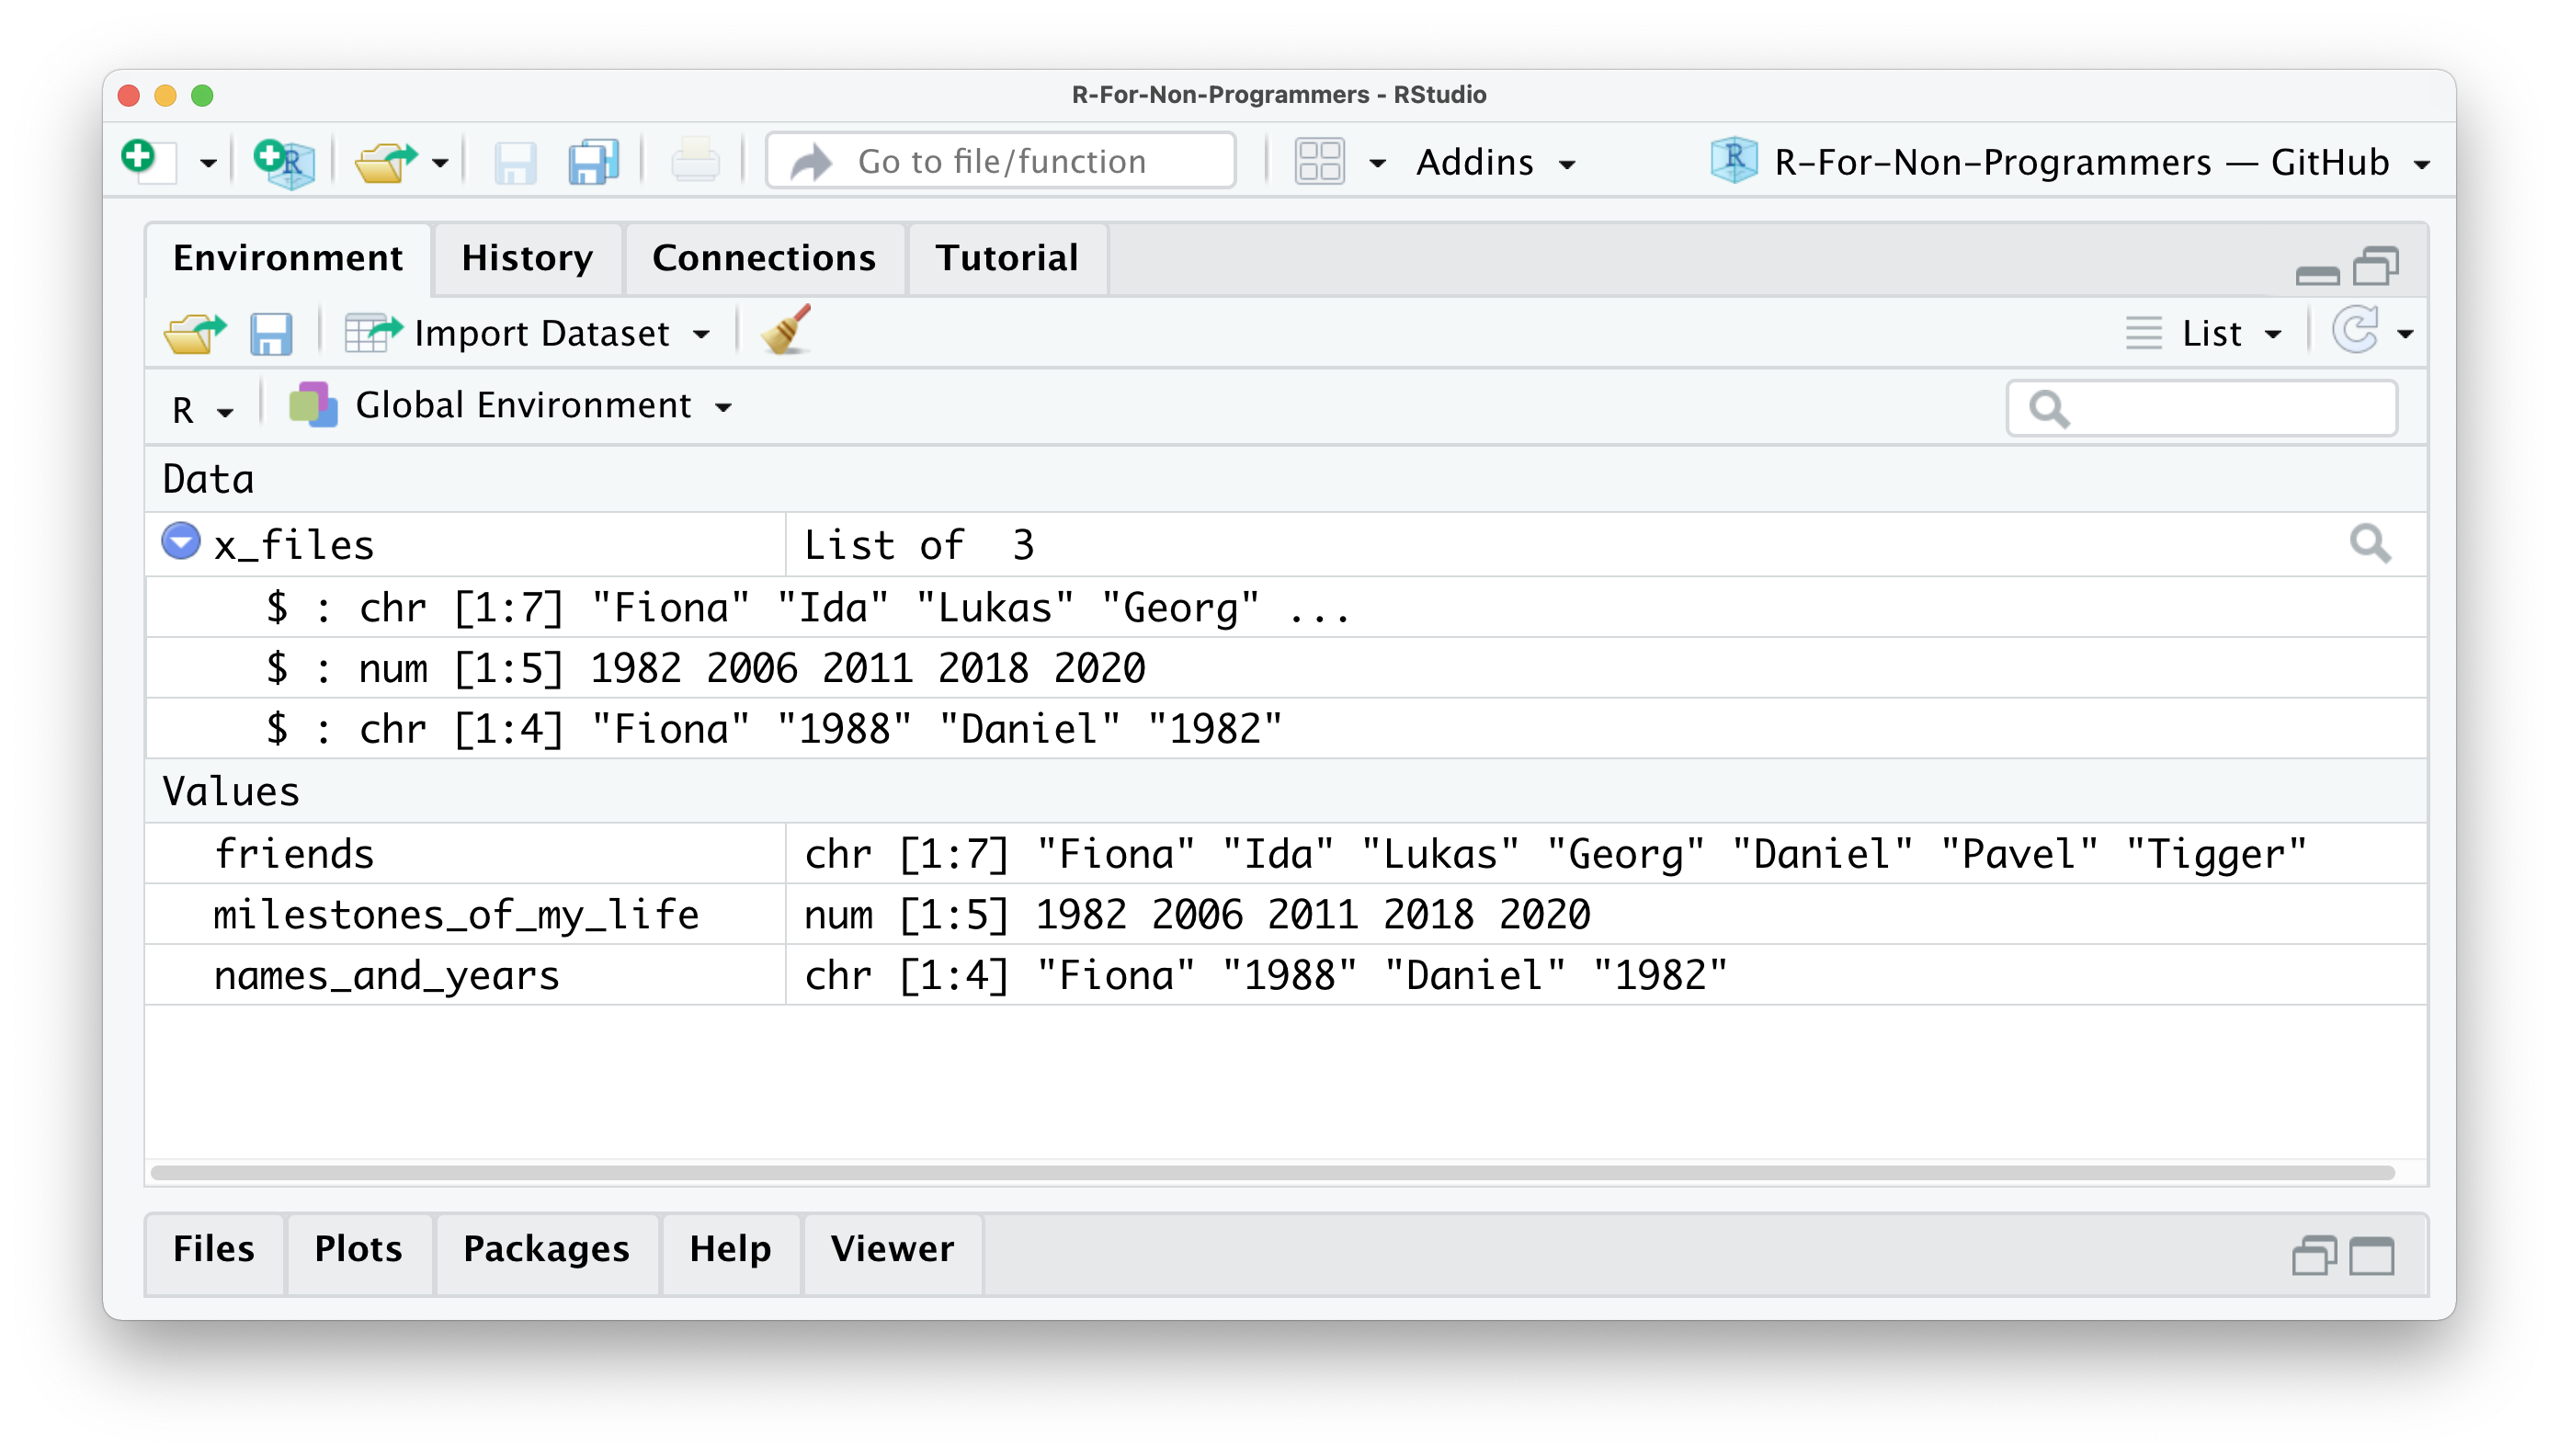
\includegraphics{images/chapter_05_img/02_basic_computation_environment_lists.png}

In Chapter \ref{basic-computations-in-r} I mentioned that we should avoid using the \texttt{=} operator and explained that it is used to assign values to objects. You can, if you want, use \texttt{=} instead of \texttt{\textless{}-}. They fulfil the same purpose. However, as mentioned before, it is not wise to do so. Here is an example that shows that, in principle, it is possible.

\begin{Shaded}
\begin{Highlighting}[]
\CommentTok{\# DO}
\NormalTok{(avengers1 }\OtherTok{\textless{}{-}} \FunctionTok{c}\NormalTok{(}\StringTok{"Iron Man"}\NormalTok{, }\StringTok{"Captain America"}\NormalTok{, }\StringTok{"Black Widow"}\NormalTok{, }\StringTok{"Vision"}\NormalTok{))}
\DocumentationTok{\#\# [1] "Iron Man"        "Captain America" "Black Widow"     "Vision"}

\CommentTok{\# DON\textquotesingle{}T}
\NormalTok{(}\AttributeTok{avengers2 =} \FunctionTok{c}\NormalTok{(}\StringTok{"Iron Man"}\NormalTok{, }\StringTok{"Captain America"}\NormalTok{, }\StringTok{"Black Widow"}\NormalTok{, }\StringTok{"Vision"}\NormalTok{))}
\DocumentationTok{\#\# [1] "Iron Man"        "Captain America" "Black Widow"     "Vision"}
\end{Highlighting}
\end{Shaded}

On a final note, naming your objects is limited. Not every name can be chosen. First, every name needs to start with a letter. You also can only use letters, numbers \texttt{\_} and \texttt{.} as valid components of the names of your objects \citep[see also][Chapter 4.2.]{wickham2016r}.

\hypertarget{functions}{%
\section{Functions}\label{functions}}

I used the term `function' multiple times already, but I never really fully explained what they are and why we need them. In very simple terms, functions are objects. They contain lines of code that someone has written for us (ro we have written ourselves). One could say they are code snippets ready to use. Someone else might see them as shortcuts for our programming. Functions not only increase the speed with which we perform our analysis and write our computations, but also make our code more readable. Consider computing the \texttt{mean} of values stored in the object \texttt{pocket\_money}.

\begin{Shaded}
\begin{Highlighting}[]
\CommentTok{\# First we create an object that stores our desired values}
\NormalTok{pocket\_money }\OtherTok{\textless{}{-}} \FunctionTok{c}\NormalTok{(}\DecValTok{0}\NormalTok{, }\DecValTok{1}\NormalTok{, }\DecValTok{1}\NormalTok{, }\DecValTok{2}\NormalTok{, }\DecValTok{3}\NormalTok{, }\DecValTok{5}\NormalTok{, }\DecValTok{8}\NormalTok{, }\DecValTok{13}\NormalTok{, }\DecValTok{21}\NormalTok{, }\DecValTok{34}\NormalTok{, }\DecValTok{55}\NormalTok{, }\DecValTok{89}\NormalTok{)}

\CommentTok{\#1 Manually compute the mean:}
\NormalTok{sum }\OtherTok{\textless{}{-}} \DecValTok{0}\SpecialCharTok{+}\DecValTok{1}\SpecialCharTok{+}\DecValTok{1}\SpecialCharTok{+}\DecValTok{2}\SpecialCharTok{+}\DecValTok{3}\SpecialCharTok{+}\DecValTok{5}\SpecialCharTok{+}\DecValTok{8}\SpecialCharTok{+}\DecValTok{13}\SpecialCharTok{+}\DecValTok{21}\SpecialCharTok{+}\DecValTok{34}\SpecialCharTok{+}\DecValTok{55}\SpecialCharTok{+}\DecValTok{89}
\NormalTok{sum}\SpecialCharTok{/}\DecValTok{12} \CommentTok{\# There are 12 items in the object}
\DocumentationTok{\#\# [1] 19.33333}

\CommentTok{\#2 Use a function to compute the mean:}
\FunctionTok{mean}\NormalTok{(pocket\_money)}
\DocumentationTok{\#\# [1] 19.33333}

\CommentTok{\#3 Let\textquotesingle{}s make sure it is actually the same}
\NormalTok{sum}\SpecialCharTok{/}\DecValTok{12} \SpecialCharTok{==} \FunctionTok{mean}\NormalTok{(pocket\_money)}
\DocumentationTok{\#\# [1] TRUE}
\end{Highlighting}
\end{Shaded}

If we manually compute the mean, we first compute the sum of all values in the object \texttt{pocket\_money}\footnote{If you find the order of numbers suspicious, it is because it represents the famous \href{https://en.wikipedia.org/wiki/Fibonacci_number}{Fibonacci sequence}.}, and then we divide it by the number of values in the object, which is \texttt{12}. This is the classic way of computing the mean as we know it. However, my simply using the function \texttt{mean()}, we not only write considerably less code, it is much easer to understand as well, because the word \texttt{mean} does exactly what we would expect. Which one do you find easier?

All functions in R share the same structure. They have a \texttt{name} follow by \texttt{()} and within these parentheses we put \texttt{arguments}, which have certain \texttt{values}. A function would look something like this:

\begin{Shaded}
\begin{Highlighting}[]
\FunctionTok{name\_of\_function}\NormalTok{(}\AttributeTok{argument\_1 =}\NormalTok{ value\_1,}
                 \AttributeTok{argument\_2 =}\NormalTok{ value\_2,}
                 \AttributeTok{argument\_3 =}\NormalTok{ value\_3)}
\end{Highlighting}
\end{Shaded}

How many arguments there are and what kind of values you can provide is very much dependent on the function you use. Thus, not every function takes every value. It is fair to make the analogy that function names are similar to vocabulary of a foreign language, while the arguments represent a specific syntax that goes with it. In the case of \texttt{mean()}, the function takes an object which holds a sequence of \texttt{numeric} values. It would make very little sense to compute the mean of our \texttt{friends} object, because it only contains names. R would return an error message:

\begin{Shaded}
\begin{Highlighting}[]
\FunctionTok{mean}\NormalTok{(friends)}
\DocumentationTok{\#\# Warning in mean.default(friends): argument is not numeric or logical: returning}
\DocumentationTok{\#\# NA}
\DocumentationTok{\#\# [1] NA}
\end{Highlighting}
\end{Shaded}

\texttt{NA} refers to a value that is \emph{`not available'}. In this case, R tries to compute the mean but the result is not available. However, it can run the function \texttt{mean()}. Therefore, this value is \texttt{NA}. In your dataset, you might find cells that are \texttt{NA}, which means there is data missing. You will learn more about how to deal with this in Chapter @ref().

Sometimes you will also get a message from R that something is \texttt{NaN}. This stands for \emph{`not a number'} and is returned when something is not possible to compute, for example:

\begin{Shaded}
\begin{Highlighting}[]

\CommentTok{\# Example 1}
\DecValTok{0}\SpecialCharTok{/}\DecValTok{0}
\DocumentationTok{\#\# [1] NaN}

\CommentTok{\# Example 2}
\FunctionTok{sqrt}\NormalTok{(}\SpecialCharTok{{-}}\DecValTok{9}\NormalTok{)}
\DocumentationTok{\#\# Warning in sqrt({-}9): NaNs produced}
\DocumentationTok{\#\# [1] NaN}
\end{Highlighting}
\end{Shaded}

\hypertarget{r-packages}{%
\section{R packages}\label{r-packages}}

R has many built-in functions that we can use right away. However, some of the most interesting ones are actually developed by other programmers, data scientists and enthusiasts. To add more functions to your repertoire, you can install R packages. R packages are a collection of functions that you can download and use for your own analysis. Throughout this book you will learn about and use many different R packages to accomplish different tasks.

To give you another analogy,

\begin{itemize}
\item
  R is like a global supermarket,
\item
  RStudio is like my shopping cart,
\item
  and R packages are the products I can pick from the shelves.
\end{itemize}

Luckily, R packages are free to use, so I do not have to bring my credit card. For me, these additional functions, developed by some of the greatest scientists, is what keeps me addicted to performing my research in R.

However, how do you find those R packages? They are right at your fingertips. You have mainly two options:

\begin{enumerate}
\def\labelenumi{\arabic{enumi}.}
\tightlist
\item
  Use the Packages pane (see Chapter \ref{the-files-plots-packages-help-viewer-window})
\item
  Or call a function
\end{enumerate}

\hypertarget{installing-packages-via-rstudios-package-pane}{%
\subsection{Installing packages via RStudio's Package pane}\label{installing-packages-via-rstudios-package-pane}}

\texttt{to\ be\ added}

\hypertarget{installing-packages-using-a-function}{%
\subsection{Installing packages using a function}\label{installing-packages-using-a-function}}

The simplest and fastest way to install a package is calling the function \texttt{install.packages()}. You can either use it to install a single package or install a series of packages all at once using our trusty \texttt{c()} function.

\begin{Shaded}
\begin{Highlighting}[]
\CommentTok{\# Install a single package}
\FunctionTok{install.packages}\NormalTok{(}\StringTok{"tidyverse"}\NormalTok{)}

\CommentTok{\# Installe multiple packages at once}
\FunctionTok{install.packages}\NormalTok{(}\FunctionTok{c}\NormalTok{(}\StringTok{"tidyverse"}\NormalTok{, }\StringTok{"naniar"}\NormalTok{, }\StringTok{"psych"}\NormalTok{))}
\end{Highlighting}
\end{Shaded}

\hypertarget{exercises-chapter-5}{%
\section{Exercises}\label{exercises-chapter-5}}

\begin{enumerate}
\def\labelenumi{\arabic{enumi}.}
\item
  What is the result of \(\sqrt[2]{25-16}+2*8-6\)?
\item
  What does the console return if you execute the following code \texttt{"Five"\ ==\ 5}?
\item
  Create a list called \texttt{books} and include the folKlowing book titles in it:

  \begin{itemize}
  \item
    ``Harry Potter and the Deathly Hallows'',
  \item
    ``The Alchemist'',
  \item
    ``The Davinci Code'',
  \item
    ``R For Dummies''
  \end{itemize}
\end{enumerate}

Check you answers: \ref{solutions-for-refexercises}

\hypertarget{exercises-solutions}{%
\chapter{Exercises: Solutions}\label{exercises-solutions}}

\hypertarget{solutions-for-refexercises}{%
\section{Solutions for \ref{exercises}}\label{solutions-for-refexercises}}

\begin{Shaded}
\begin{Highlighting}[]
\CommentTok{\#1}
\FunctionTok{sqrt}\NormalTok{(}\DecValTok{25{-}16}\NormalTok{)}\SpecialCharTok{+}\DecValTok{2}\SpecialCharTok{*}\DecValTok{8{-}6}
\DocumentationTok{\#\# [1] 13}

\CommentTok{\#2}
\StringTok{"Five"} \SpecialCharTok{==} \DecValTok{5}
\DocumentationTok{\#\# [1] FALSE}

\CommentTok{\#3 }
\NormalTok{books }\OtherTok{\textless{}{-}} \FunctionTok{list}\NormalTok{(}\StringTok{"Harry Potter and the Deathly Hallows"}\NormalTok{,}
              \StringTok{"The Alchemist"}\NormalTok{,}
              \StringTok{"The Davinci Code"}\NormalTok{,}
              \StringTok{"R For Dummies"}\NormalTok{)}

\NormalTok{books}
\DocumentationTok{\#\# [[1]]}
\DocumentationTok{\#\# [1] "Harry Potter and the Deathly Hallows"}
\DocumentationTok{\#\# }
\DocumentationTok{\#\# [[2]]}
\DocumentationTok{\#\# [1] "The Alchemist"}
\DocumentationTok{\#\# }
\DocumentationTok{\#\# [[3]]}
\DocumentationTok{\#\# [1] "The Davinci Code"}
\DocumentationTok{\#\# }
\DocumentationTok{\#\# [[4]]}
\DocumentationTok{\#\# [1] "R For Dummies"}
\end{Highlighting}
\end{Shaded}


  \bibliography{book.bib,packages.bib}

\end{document}
